\section{Casi d'uso}
\subsection{Introduzione}
In questa sezione del documento vengono analizzati nel dettaglio i casi d'uso individuati in fase di analisi del \href{https://7last.github.io/docs/pb/documentazione-interna/glossario\#capitolato}{capitolato\textsubscript{G}} e durante i colloqui con il \href{https://7last.github.io/docs/pb/documentazione-interna/glossario\#proponente}{proponente\textsubscript{G}}.

\subsection{Struttura dei casi d'uso}
In tutto il documento faremo riferimento ai casi d'uso utilizzando la sigla \texttt{UC} seguita dal rispettivo codice nella forma
\begin{center}
	\textbf{UC-[identificativo\_caso\_principale].[identificativo\_sotto\_caso]}
\end{center}
il quale permette di utilizzarlo come riferimento in questo e in altri documenti.\\
Per ciascun caso d'uso vengono definiti i seguenti elementi:
\begin{itemize}
	\item \textbf{attore principale}, entità primariamente coinvolta nel caso d'uso;
	\item \textbf{precondizioni}, le condizioni che devono essere verificate prima che il caso d'uso possa essere eseguito;
	\item \textbf{postcondizioni}, le condizioni che devono essere verificate al termine dell'esecuzione del caso;
	\item \textbf{scenario principale}, la sequenza di passi che descrive il comportamento del sistema durante l'esecuzione del caso d'uso;
	\item \href{https://7last.github.io/docs/pb/documentazione-interna/glossario\#user-story}{\textbf{user story}\textsubscript{G}}: una descrizione testuale del caso d'uso.
\end{itemize}

\subsection{Attori}
I seguenti attori sono coinvolti nei casi d'uso:
\begin{itemize}
	\item \textbf{autorità locali}, possono accedere al sistema per visualizzare i dati di monitoraggio della \href{https://7last.github.io/docs/pb/documentazione-interna/glossario\#smart-city}{\textit{Smart City}\textsubscript{G}};
	\item \textbf{sensori}, sorgente di dati con un determinato dominio di interesse che effettua misurazioni e trasmette i dati al sistema.
\end{itemize}

\subsection{Elenco dei casi d'uso}
\subsubsection{UC-1: Visualizzazione dashboard}
\begin{itemize}
	\item \textbf{Attore principale}: autorità locale.
	\item \textbf{Precondizioni}: l'autorità locale ha effettuato l'accesso al sistema ed esso è in funzione.
	\item \textbf{Postcondizioni}: l'autorità locale visualizza la \href{https://7last.github.io/docs/pb/documentazione-interna/glossario\#dashboard}{dashboard\textsubscript{G}} con i dati relativi ai sensori presenti nella città.
	\item \textbf{Scenario principale}:
	      \begin{enumerate}
		      \item l'autorità locale accede alla piattaforma.
		      \item il sistema carica i dati relativi ai sensori interrogando il database.
	      \end{enumerate}
	\item \href{https://7last.github.io/docs/pb/documentazione-interna/glossario\#user-story}{\textbf{User story}\textsubscript{G}}:
	      come autorità locale desidero poter visualizzare una \href{https://7last.github.io/docs/pb/documentazione-interna/glossario\#dashboard}{dashboard\textsubscript{G}} con i dati relativi ai sensori per poter monitorare la loro posizione e i dati trasmessi.
\end{itemize}
\begin{center}
	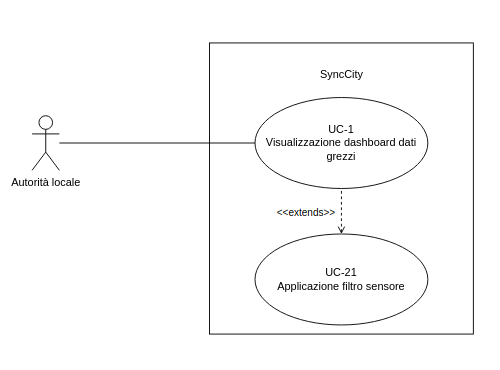
\includegraphics[width=0.5\textwidth]{analisi_dei_requisiti/UC-1.png}
	\captionof{figure}{UC-1: Visualizzazione \href{https://7last.github.io/docs/pb/documentazione-interna/glossario\#dashboard}{dashboard\textsubscript{G}}}
\end{center}

\newpage
\subsubsection{UC-2: Visualizzazione dashboard dati grezzi}
\begin{itemize}
	\item \textbf{Attore principale}: autorità locale.
	\item \textbf{Precondizioni}: l'autorità locale ha effettuato l'accesso al sistema ed esso è in funzione.
	\item \textbf{Postcondizioni}: l'autorità locale visualizza la \href{https://7last.github.io/docs/pb/documentazione-interna/glossario\#dashboard}{dashboard\textsubscript{G}} dei dati grezzi con i dati relativi ai sensori presenti nella città, mostrando il \href{https://7last.github.io/docs/pb/documentazione-interna/glossario\#panel}{\textit{panel}\textsubscript{G}} con la tabella di tutti i sensori collegati al sistema, la mappa interattiva popolata con dei \textit{marker}, il \textit{panel} con il conteggio totale di sensori per tipologia, la tabella dei sensori che non trasmettono da più di un giorno e, per ciascuna tipologia di sensore (temperatura, umidità, traffico, qualità dell'aria, precipitazioni, isole ecologiche, livello dei fiumi e colonnine di ricarica) una tabella con i dati grezzi trasmessi e un grafico time series.
	\item \textbf{Scenario principale}:
	      \begin{enumerate}
		      \item l'autorità locale accede alla piattaforma;
		      \item il sistema carica i dati relativi ai sensori interrogando il database.
	      \end{enumerate}
	\item \href{https://7last.github.io/docs/pb/documentazione-interna/glossario\#user-story}{\textbf{User story}\textsubscript{G}}: come autorità locale desidero poter visualizzare una \href{https://7last.github.io/docs/pb/documentazione-interna/glossario\#dashboard}{dashboard\textsubscript{G}} dei dati grezzi con i dati relativi ai sensori presenti nella città, potendo vedere il \href{https://7last.github.io/docs/pb/documentazione-interna/glossario\#panel}{\textit{panel}\textsubscript{G}} con la tabella di tutti i sensori collegati al sistema, la mappa interattiva popolata con dei \textit{marker}, il \textit{panel} con il conteggio totale di sensori per tipologia, la tabella dei sensori che non trasmettono da più di un giorno e, per ciascuna tipologia di sensore (temperatura, umidità, traffico, qualità dell'aria, precipitazioni, isole ecologiche, livello dei fiumi e colonnine di ricarica) una tabella con i dati grezzi trasmessi e un grafico time series.
\end{itemize}
\begin{center}
	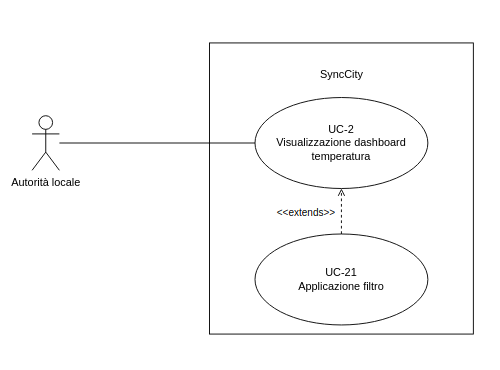
\includegraphics[width=0.5\textwidth]{analisi_dei_requisiti/UC-2.png}
	\captionof{figure}{UC-2: Visualizzazione \href{https://7last.github.io/docs/pb/documentazione-interna/glossario\#dashboard}{dashboard\textsubscript{G}} dei dati grezzi}
\end{center}

\newpage
\subsubsubsection{UC-2.1: Visualizzazione \textit{panel} con tabella sensori}
\begin{itemize}
	\item \textbf{Attore principale}: autorità locale.
	\item \textbf{Precondizioni}: l'autorità locale ha effettuato l'accesso al sistema ed esso è in funzione.
	\item \textbf{Postcondizioni}: l'autorità locale visualizza il \href{https://7last.github.io/docs/pb/documentazione-interna/glossario\#panel}{\textit{panel}\textsubscript{G}} contenente una tabella di tutti i sensori collegati al sistema,
	      in cui sono presenti l'identificativo del \href{https://7last.github.io/docs/pb/documentazione-interna/glossario\#sensore}{sensore\textsubscript{G}}, il tipo di \href{https://7last.github.io/docs/pb/documentazione-interna/glossario\#sensore}{sensore\textsubscript{G}} e la data dell'ultima trasmissione.
	\item \textbf{Scenario principale}:
	      \begin{enumerate}
		      \item l'autorità locale accede alla piattaforma;
		      \item il sistema carica i dati relativi ai sensori interrogando il database;
		      \item l'autorità locale seleziona la visualizzazione della \href{https://7last.github.io/docs/pb/documentazione-interna/glossario\#dashboard}{dashboard\textsubscript{G}} dei dati grezzi.
	      \end{enumerate}
	\item \href{https://7last.github.io/docs/pb/documentazione-interna/glossario\#user-story}{\textbf{User story}\textsubscript{G}}: come autorità locale desidero poter visualizzare un \href{https://7last.github.io/docs/pb/documentazione-interna/glossario\#panel}{\textit{panel}\textsubscript{G}} contenente una tabella di tutti i sensori collegati al sistema. I dati che devono essere presenti nella tabella sono: identificativo del \href{https://7last.github.io/docs/pb/documentazione-interna/glossario\#sensore}{sensore\textsubscript{G}}, tipo di \href{https://7last.github.io/docs/pb/documentazione-interna/glossario\#sensore}{sensore\textsubscript{G}} e data dell'ultima trasmissione. Questi mi consentiranno di avere una visione d'insieme dei sensori presenti.
\end{itemize}
\begin{center}
	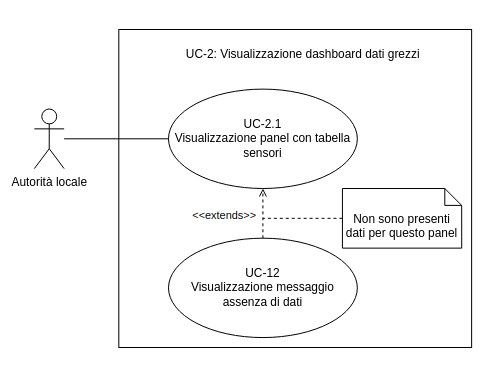
\includegraphics[width=0.5\textwidth]{analisi_dei_requisiti/UC-2.1.png}
	\captionof{figure}{UC-2.1: Visualizzazione \href{https://7last.github.io/docs/pb/documentazione-interna/glossario\#panel}{\textit{panel}\textsubscript{G}} con tabella sensori}
\end{center}

\newpage
\subsubsubsection{UC-2.2: Visualizzazione mappa interattiva sensori}
\begin{itemize}
	\item \textbf{Attore principale}: autorità locale.
	\item \textbf{Precondizioni}: l'autorità locale ha effettuato l'accesso al sistema ed esso è in funzione.
	\item \textbf{Postcondizioni}: l'autorità locale visualizza un \href{https://7last.github.io/docs/pb/documentazione-interna/glossario\#panel}{\textit{panel}\textsubscript{G}} contenente una mappa interattiva
	      popolata con dei \textit{marker}. Ogni marker consente di visualizzare l'identificativo del \href{https://7last.github.io/docs/pb/documentazione-interna/glossario\#sensore}{sensore\textsubscript{G}} e le sue coordinate geografiche.
	\item \textbf{Scenario principale}:
	      \begin{enumerate}
		      \item l'autorità locale accede alla piattaforma;
		      \item il sistema carica i dati trasmessi dai sensori interrogando il database;
		      \item l'autorità locale seleziona la visualizzazione della \href{https://7last.github.io/docs/pb/documentazione-interna/glossario\#dashboard}{dashboard\textsubscript{G}} dei dati grezzi.
	      \end{enumerate}
	\item \href{https://7last.github.io/docs/pb/documentazione-interna/glossario\#user-story}{\textbf{User story}\textsubscript{G}}: come autorità locale desidero poter visualizzare una mappa interattiva popolata con dei \textit{marker} rappresentanti
	      la posizione dei sensori e contenenti il loro identificativo. Essa mi consentirà di visualizzare la distribuzione dei sensori nel territorio
	      ed eventualmente di intervenire nel caso in cui siano presenti zone non coperte.
\end{itemize}
\begin{center}
	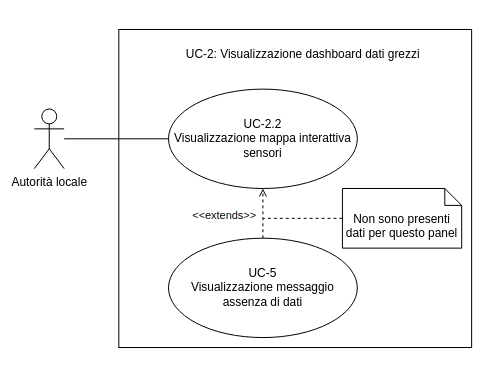
\includegraphics[width=0.5\textwidth]{analisi_dei_requisiti/UC-2.2.png}
	\captionof{figure}{UC-2.2: Visualizzazione mappa interattiva sensori}
\end{center}


\newpage
\subsubsubsection{UC-2.3: Visualizzazione \textit{panel} numero sensori per tipo}
\begin{itemize}
	\item \textbf{Attore principale}: autorità locale.
	\item \textbf{Precondizioni}: l'autorità locale ha effettuato l'accesso al sistema ed esso è in funzione.
	\item \textbf{Postcondizioni}: l'autorità locale visualizza un \href{https://7last.github.io/docs/pb/documentazione-interna/glossario\#panel}{\textit{panel}\textsubscript{G}} contenente il conteggio totale di sensori presenti nel sistema, suddivisi per tipologia.
	\item \textbf{Scenario principale}:
	      \begin{enumerate}
		      \item l'autorità locale accede alla piattaforma;
		      \item il sistema carica i dati trasmessi dai sensori interrogando il database;
		      \item l'autorità locale seleziona la visualizzazione della \href{https://7last.github.io/docs/pb/documentazione-interna/glossario\#dashboard}{dashboard\textsubscript{G}} dei dati grezzi.
	      \end{enumerate}
	\item \href{https://7last.github.io/docs/pb/documentazione-interna/glossario\#user-story}{\textbf{User story}\textsubscript{G}}:
	      come autorità locale, desidero visualizzare il conteggio totale dei sensori presenti nel sistema, suddivisi per tipologia, per poter valutare l'eventuale necessità di aggiungerne altri.
\end{itemize}
\begin{center}
	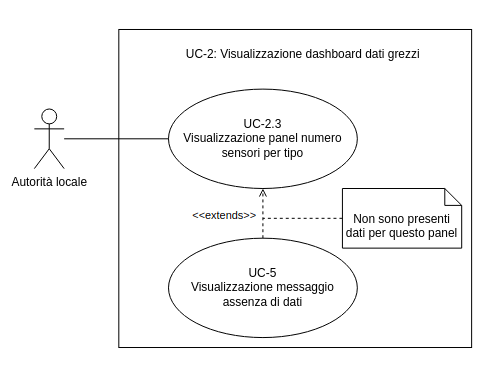
\includegraphics[width=0.5\textwidth]{analisi_dei_requisiti/UC-2.3.png}
	\captionof{figure}{UC-2.3: Visualizzazione \href{https://7last.github.io/docs/pb/documentazione-interna/glossario\#panel}{\textit{panel}\textsubscript{G}} numero sensori per tipo}
\end{center}

\newpage
\subsubsubsection{UC-2.4: Visualizzazione tabella sensori non trasmettenti}
\begin{itemize}
	\item \textbf{Attore principale}: autorità locale.
	\item \textbf{Precondizioni}: l'autorità locale ha effettuato l'accesso al sistema ed esso è in funzione.
	\item \textbf{Postcondizioni}: l'autorità locale visualizza una tabella contenente i sensori che non trasmettono da più di un giorno. Ciascuna riga
	      contiene il nome del \href{https://7last.github.io/docs/pb/documentazione-interna/glossario\#sensore}{sensore\textsubscript{G}}, il tipo di \href{https://7last.github.io/docs/pb/documentazione-interna/glossario\#sensore}{sensore\textsubscript{G}} e la data dell'ultima trasmissione.
	\item \textbf{Scenario principale}:
	      \begin{enumerate}
		      \item l'autorità locale accede alla piattaforma;
		      \item il sistema carica i dati trasmessi dai sensori interrogando il database;
		      \item l'autorità locale seleziona la visualizzazione della \href{https://7last.github.io/docs/pb/documentazione-interna/glossario\#dashboard}{dashboard\textsubscript{G}} dei dati grezzi.
	      \end{enumerate}
	\item \href{https://7last.github.io/docs/pb/documentazione-interna/glossario\#user-story}{\textbf{User story}\textsubscript{G}}:
	      come autorità locale desidero poter visualizzare una tabella contenente i sensori che non trasmettono da più di un giorno, contenente
	      il nome del \href{https://7last.github.io/docs/pb/documentazione-interna/glossario\#sensore}{sensore\textsubscript{G}}, il tipo di \href{https://7last.github.io/docs/pb/documentazione-interna/glossario\#sensore}{sensore\textsubscript{G}} e la data dell'ultima trasmissione, in modo da poter intervenire e ripristinare il corretto funzionamento.
\end{itemize}
\begin{center}
	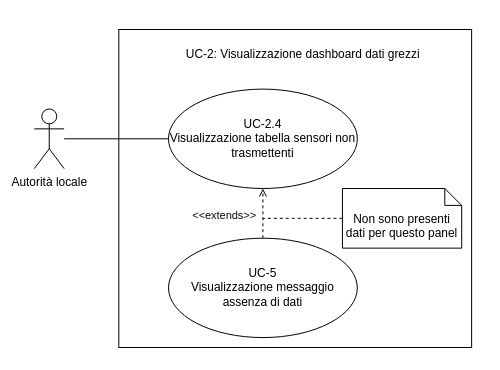
\includegraphics[width=0.5\textwidth]{analisi_dei_requisiti/UC-2.4.png}
	\captionof{figure}{UC-2.4: Visualizzazione tabella sensori che non trasmettono da più di 1 giorno}
\end{center}

\newpage
\subsubsubsection{UC-2.5: Visualizzazione tabella dati grezzi temperatura}
\begin{itemize}
	\item \textbf{Attore principale}: autorità locale.
	\item \textbf{Precondizioni}: l'autorità locale ha effettuato l'accesso al sistema ed esso è in funzione.
	\item \textbf{Postcondizioni}: l'autorità locale visualizza una tabella contenente i dati grezzi trasmessi dai sensori di temperatura.
	      Ciascuna riga contiene il nome del \href{https://7last.github.io/docs/pb/documentazione-interna/glossario\#sensore}{sensore\textsubscript{G}}, il valore della temperatura in gradi Celsius e il timestamp della trasmissione.
	\item \textbf{Scenario principale}:
	      \begin{enumerate}
		      \item l'autorità locale accede alla piattaforma;
		      \item il sistema carica i dati trasmessi dai sensori interrogando il database;
		      \item l'autorità locale seleziona la visualizzazione della \href{https://7last.github.io/docs/pb/documentazione-interna/glossario\#dashboard}{dashboard\textsubscript{G}} dei dati grezzi.
	      \end{enumerate}
	\item \href{https://7last.github.io/docs/pb/documentazione-interna/glossario\#user-story}{\textbf{User story}\textsubscript{G}}:
	      come autorità locale desidero poter visualizzare una tabella contenente i dati grezzi delle misurazioni di temperatura
	      in gradi Celsius, il nome del \href{https://7last.github.io/docs/pb/documentazione-interna/glossario\#sensore}{sensore\textsubscript{G}} e il timestamp della trasmissione, in modo da poter analizzare i dati in modo più dettagliato.
\end{itemize}
\begin{center}
	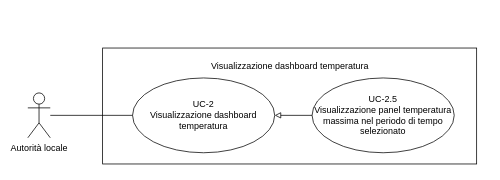
\includegraphics[width=0.5\textwidth]{analisi_dei_requisiti/UC-2.5.png}
	\captionof{figure}{UC-2.5: Visualizzazione tabella dati grezzi temperatura}
\end{center}

\newpage
\subsubsubsection{UC-2.6: Visualizzazione tabella dati grezzi umidità}
\begin{itemize}
	\item \textbf{Attore principale}: autorità locale.
	\item \textbf{Precondizioni}: l'autorità locale ha effettuato l'accesso al sistema ed esso è in funzione.
	\item \textbf{Postcondizioni}: l'autorità locale visualizza una tabella contenente i dati grezzi trasmessi dai sensori di umidità.
	      Ciascuna riga contiene il nome del \href{https://7last.github.io/docs/pb/documentazione-interna/glossario\#sensore}{sensore\textsubscript{G}}, il valore dell'umidità in percentuale e il timestamp della trasmissione.
	\item \textbf{Scenario principale}:
	      \begin{enumerate}
		      \item l'autorità locale accede alla piattaforma;
		      \item il sistema carica i dati trasmessi dai sensori interrogando il database;
		      \item l'autorità locale seleziona la visualizzazione della \href{https://7last.github.io/docs/pb/documentazione-interna/glossario\#dashboard}{dashboard\textsubscript{G}} dei dati grezzi.
	      \end{enumerate}
	\item \href{https://7last.github.io/docs/pb/documentazione-interna/glossario\#user-story}{\textbf{User story}\textsubscript{G}}:
	      come autorità locale desidero poter visualizzare una tabella contenente i dati grezzi delle misurazioni di umidità in percentuale,
	      il nome del \href{https://7last.github.io/docs/pb/documentazione-interna/glossario\#sensore}{sensore\textsubscript{G}} e il timestamp della trasmissione, in modo da poter analizzare i dati in modo più dettagliato.
\end{itemize}
\begin{center}
	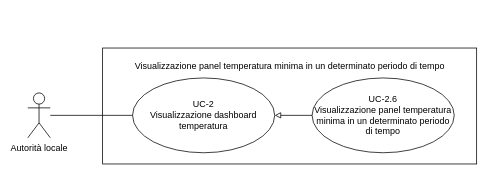
\includegraphics[width=0.5\textwidth]{analisi_dei_requisiti/UC-2.6.png}
	\captionof{figure}{UC-2.6: Visualizzazione tabella dati grezzi umidità}
\end{center}

\newpage
\subsubsubsection{UC-2.7: Visualizzazione tabella dati grezzi traffico}
\begin{itemize}
	\item \textbf{Attore principale}: autorità locale.
	\item \textbf{Precondizioni}: l'autorità locale ha effettuato l'accesso al sistema ed esso è in funzione.
	\item \textbf{Postcondizioni}: l'autorità locale visualizza una tabella contenente i dati grezzi trasmessi dai sensori di traffico.
	      Ciascuna riga contiene il nome del \href{https://7last.github.io/docs/pb/documentazione-interna/glossario\#sensore}{sensore\textsubscript{G}}, il numero di veicoli transitati, la loro velocità media espressa in km/h e il timestamp della trasmissione.
	\item \textbf{Scenario principale}:
	      \begin{enumerate}
		      \item l'autorità locale accede alla piattaforma;
		      \item il sistema carica i dati trasmessi dai sensori interrogando il database;
		      \item l'autorità locale seleziona la visualizzazione della \href{https://7last.github.io/docs/pb/documentazione-interna/glossario\#dashboard}{dashboard\textsubscript{G}} dei dati grezzi.
	      \end{enumerate}
	\item \href{https://7last.github.io/docs/pb/documentazione-interna/glossario\#user-story}{\textbf{User story}\textsubscript{G}}:
	      come autorità locale desidero poter visualizzare una tabella contenente i dati grezzi delle misurazioni del numero di veicoli transitati
	      e della velocità media espressa in km/h, il nome del \href{https://7last.github.io/docs/pb/documentazione-interna/glossario\#sensore}{sensore\textsubscript{G}} e il timestamp della trasmissione, in modo da poter analizzare i dati in modo più dettagliato.
\end{itemize}
\begin{center}
	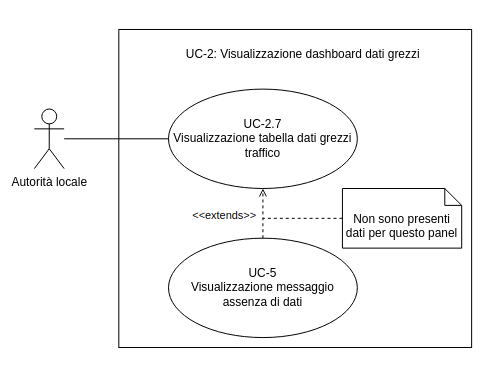
\includegraphics[width=0.5\textwidth]{analisi_dei_requisiti/UC-2.7.png}
	\captionof{figure}{UC-2.7: Visualizzazione tabella dati grezzi traffico}
\end{center}

\newpage
\subsubsubsection{UC-2.8: Visualizzazione tabella dati grezzi qualità dell'aria}
\begin{itemize}
	\item \textbf{Attore principale}: autorità locale.
	\item \textbf{Precondizioni}: l'autorità locale ha effettuato l'accesso al sistema ed esso è in funzione.
	\item \textbf{Postcondizioni}: l'autorità locale visualizza una tabella contenente i dati grezzi trasmessi dai sensori di qualità dell'aria.
	      Ciascuna riga contiene il nome del \href{https://7last.github.io/docs/pb/documentazione-interna/glossario\#sensore}{sensore\textsubscript{G}}, il valore in $\mu g/m^3$ di PM10, PM2.5, NO\textsubscript{2}, O\textsubscript{3}, SO\textsubscript{2} e il timestamp della trasmissione.
	\item \textbf{Scenario principale}:
	      \begin{enumerate}
		      \item l'autorità locale accede alla piattaforma;
		      \item il sistema carica i dati trasmessi dai sensori interrogando il database;
		      \item l'autorità locale seleziona la visualizzazione della \href{https://7last.github.io/docs/pb/documentazione-interna/glossario\#dashboard}{dashboard\textsubscript{G}} dei dati grezzi.
	      \end{enumerate}
	\item \href{https://7last.github.io/docs/pb/documentazione-interna/glossario\#user-story}{\textbf{User story}\textsubscript{G}}:
	      come autorità locale desidero poter visualizzare una tabella contenente i dati grezzi delle misurazioni di PM10, PM2.5, NO\textsubscript{2}, O\textsubscript{3}, SO\textsubscript{2},
	      il nome del \href{https://7last.github.io/docs/pb/documentazione-interna/glossario\#sensore}{sensore\textsubscript{G}} e il timestamp della trasmissione, in modo da poter analizzare i dati in modo più dettagliato.
\end{itemize}
\begin{center}
	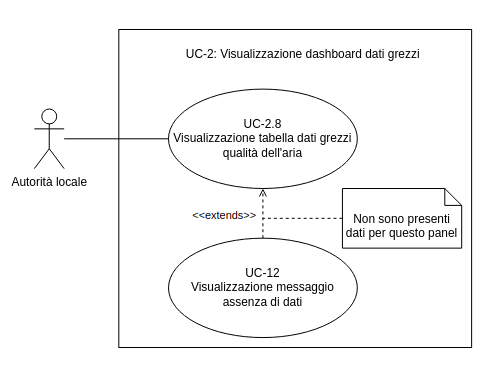
\includegraphics[width=0.5\textwidth]{analisi_dei_requisiti/UC-2.8.png}
	\captionof{figure}{UC-2.8: Visualizzazione tabella dati grezzi qualità dell'aria}
\end{center}

\newpage
\subsubsubsection{UC-2.9: Visualizzazione tabella dati grezzi precipitazioni}
\begin{itemize}
	\item \textbf{Attore principale}: autorità locale.
	\item \textbf{Precondizioni}: l'autorità locale ha effettuato l'accesso al sistema ed esso è in funzione.
	\item \textbf{Postcondizioni}: l'autorità locale visualizza una tabella contenente i dati grezzi trasmessi dai sensori di precipitazioni.
	      Ciascuna riga contiene il nome del \href{https://7last.github.io/docs/pb/documentazione-interna/glossario\#sensore}{sensore\textsubscript{G}}, il valore in mm di precipitazioni e il timestamp della trasmissione.
	\item \textbf{Scenario principale}:
	      \begin{enumerate}
		      \item l'autorità locale accede alla piattaforma;
		      \item il sistema carica i dati trasmessi dai sensori interrogando il database;
		      \item l'autorità locale seleziona la visualizzazione della \href{https://7last.github.io/docs/pb/documentazione-interna/glossario\#dashboard}{dashboard\textsubscript{G}} dei dati grezzi.
	      \end{enumerate}
	\item \href{https://7last.github.io/docs/pb/documentazione-interna/glossario\#user-story}{\textbf{User story}\textsubscript{G}}:
	      come autorità locale desidero poter visualizzare una tabella contenente i dati grezzi delle misurazioni di precipitazioni in mm,
	      il nome del \href{https://7last.github.io/docs/pb/documentazione-interna/glossario\#sensore}{sensore\textsubscript{G}} e il timestamp della trasmissione, in modo da poter analizzare i dati in modo più dettagliato.
\end{itemize}
\begin{center}
	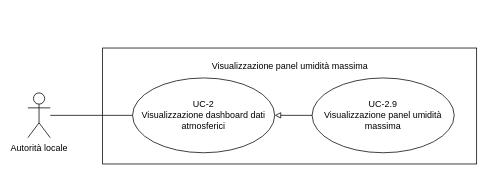
\includegraphics[width=0.5\textwidth]{analisi_dei_requisiti/UC-2.9.png}
	\captionof{figure}{UC-2.9: Visualizzazione tabella dati grezzi precipitazioni}
\end{center}

\newpage
\subsubsubsection{UC-2.10: Visualizzazione tabella dati grezzi isole ecologiche}
\begin{itemize}
	\item \textbf{Attore principale}: autorità locale.
	\item \textbf{Precondizioni}: l'autorità locale ha effettuato l'accesso al sistema ed esso è in funzione.
	\item \textbf{Postcondizioni}: l'autorità locale visualizza una tabella contenente i dati grezzi trasmessi dai sensori di isole ecologiche.
	      Ciascuna riga contiene il nome del \href{https://7last.github.io/docs/pb/documentazione-interna/glossario\#sensore}{sensore\textsubscript{G}}, il valore in percentuale di riempimento e il timestamp della trasmissione.
	\item \textbf{Scenario principale}:
	      \begin{enumerate}
		      \item l'autorità locale accede alla piattaforma;
		      \item il sistema carica i dati trasmessi dai sensori interrogando il database;
		      \item l'autorità locale seleziona la visualizzazione della \href{https://7last.github.io/docs/pb/documentazione-interna/glossario\#dashboard}{dashboard\textsubscript{G}} dei dati grezzi.
	      \end{enumerate}
	\item \href{https://7last.github.io/docs/pb/documentazione-interna/glossario\#user-story}{\textbf{User story}\textsubscript{G}}:
	      come autorità locale desidero poter visualizzare una tabella contenente i dati grezzi delle misurazioni di riempimento in percentuale delle isole ecologiche,
	      il nome del \href{https://7last.github.io/docs/pb/documentazione-interna/glossario\#sensore}{sensore\textsubscript{G}} e il timestamp della trasmissione, in modo da poter analizzare i dati in modo più dettagliato.
\end{itemize}
\begin{center}
	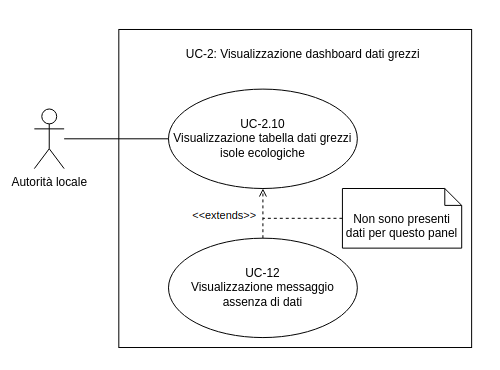
\includegraphics[width=0.5\textwidth]{analisi_dei_requisiti/UC-2.10.png}
	\captionof{figure}{UC-2.10: Visualizzazione tabella dati grezzi isole ecologiche}
\end{center}

\newpage
\subsubsubsection{UC-2.11: Visualizzazione tabella dati grezzi livello dei fiumi}
\begin{itemize}
	\item \textbf{Attore principale}: autorità locale.
	\item \textbf{Precondizioni}: l'autorità locale ha effettuato l'accesso al sistema ed esso è in funzione.
	\item \textbf{Postcondizioni}: l'autorità locale visualizza una tabella contenente i dati grezzi trasmessi dai sensori di livello dei fiumi.
	      Ciascuna riga contiene il nome del \href{https://7last.github.io/docs/pb/documentazione-interna/glossario\#sensore}{sensore\textsubscript{G}}, il valore in mm del livello dei fiumi e il timestamp della trasmissione.
	\item \textbf{Scenario principale}:
	      \begin{enumerate}
		      \item l'autorità locale accede alla piattaforma;
		      \item il sistema carica i dati trasmessi dai sensori interrogando il database;
		      \item l'autorità locale seleziona la visualizzazione della \href{https://7last.github.io/docs/pb/documentazione-interna/glossario\#dashboard}{dashboard\textsubscript{G}} dei dati grezzi.
	      \end{enumerate}
	\item \href{https://7last.github.io/docs/pb/documentazione-interna/glossario\#user-story}{\textbf{User story}\textsubscript{G}}:
	      come autorità locale desidero poter visualizzare una tabella contenente i dati grezzi delle misurazioni del livello dei fiumi in cm,
	      il nome del \href{https://7last.github.io/docs/pb/documentazione-interna/glossario\#sensore}{sensore\textsubscript{G}} e il timestamp della trasmissione, in modo da poter analizzare i dati in modo più dettagliato.
\end{itemize}
\begin{center}
	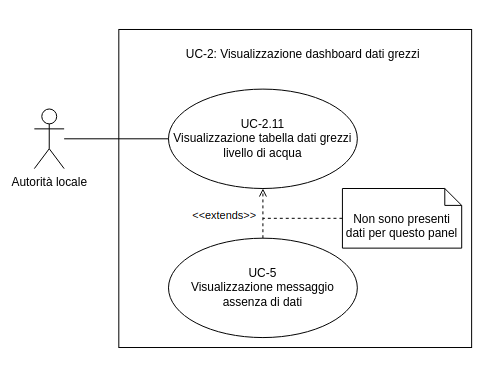
\includegraphics[width=0.5\textwidth]{analisi_dei_requisiti/UC-2.11.png}
	\captionof{figure}{UC-2.11: Visualizzazione tabella dati grezzi livello dei fiumi}
\end{center}

\newpage
\subsubsubsection{UC-2.12: Visualizzazione tabella dati grezzi colonnine di ricarica}
\begin{itemize}
	\item \textbf{Attore principale}: autorità locale.
	\item \textbf{Precondizioni}: l'autorità locale ha effettuato l'accesso al sistema ed esso è in funzione.
	\item \textbf{Postcondizioni}: l'autorità locale visualizza una tabella contenente i dati grezzi trasmessi dai sensori di colonnine di ricarica.
	      Ciascuna riga contiene il nome del \href{https://7last.github.io/docs/pb/documentazione-interna/glossario\#sensore}{sensore\textsubscript{G}}, il valore in kW della potenza erogata, il tempo rimanente alla ricarica e il timestamp della trasmissione.
	\item \textbf{Scenario principale}:
	      \begin{enumerate}
		      \item l'autorità locale accede alla piattaforma;
		      \item il sistema carica i dati trasmessi dai sensori interrogando il database;
		      \item l'autorità locale seleziona la visualizzazione della \href{https://7last.github.io/docs/pb/documentazione-interna/glossario\#dashboard}{dashboard\textsubscript{G}} dei dati grezzi.
	      \end{enumerate}
	\item \href{https://7last.github.io/docs/pb/documentazione-interna/glossario\#user-story}{\textbf{User story}\textsubscript{G}}:
	      come autorità locale desidero poter visualizzare una tabella contenente i dati grezzi delle misurazioni della potenza erogata in kW,
	      il tempo rimanente alla ricarica, il nome del \href{https://7last.github.io/docs/pb/documentazione-interna/glossario\#sensore}{sensore\textsubscript{G}} e il timestamp della trasmissione, in modo da poter analizzare i dati in modo più dettagliato.
\end{itemize}
\begin{center}
	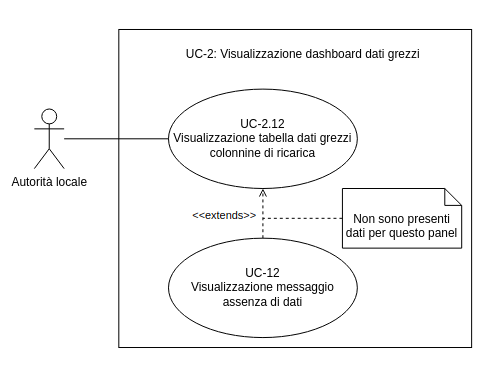
\includegraphics[width=0.5\textwidth]{analisi_dei_requisiti/UC-2.12.png}
	\captionof{figure}{UC-2.12: Visualizzazione tabella dati grezzi colonnine di ricarica}
\end{center}

\newpage
\subsubsubsection{UC-2.13: Visualizzazione grafico time series dati grezzi complessivi temperatura}
\begin{itemize}
	\item \textbf{Attore principale}: autorità locale.
	\item \textbf{Precondizioni}: l'autorità locale ha effettuato l'accesso al sistema ed esso è in funzione.
	\item \textbf{Postcondizioni}: l'autorità locale visualizza un grafico \href{https://7last.github.io/docs/pb/documentazione-interna/glossario\#time-series}{time series\textsubscript{G}} contenente i dati grezzi di temperatura trasmessi da tutti i sensori presenti nella città, mostrando sull'asse delle ascisse i timestamp delle misurazioni e su quello delle ordinate i valori delle misurazioni di temperatura in gradi Celsius.
	\item \textbf{Scenario principale}:
	      \begin{enumerate}
		      \item l'autorità locale accede alla piattaforma;
		      \item il sistema carica i dati trasmessi dai sensori interrogando il database;
		      \item l'autorità locale seleziona la visualizzazione della \href{https://7last.github.io/docs/pb/documentazione-interna/glossario\#dashboard}{dashboard\textsubscript{G}} dei dati grezzi.
	      \end{enumerate}
	\item \href{https://7last.github.io/docs/pb/documentazione-interna/glossario\#user-story}{\textbf{User story}\textsubscript{G}}:
	      come autorità locale desidero poter visualizzare un grafico \href{https://7last.github.io/docs/pb/documentazione-interna/glossario\#time-series}{time series\textsubscript{G}} contenente i dati grezzi trasmessi da tutti i sensori
	      di temperatura presenti nella città, espressi in gradi Celsius, in modo da poterli confrontare tra loro e analizzare in modo più dettagliato.
\end{itemize}
\begin{center}
	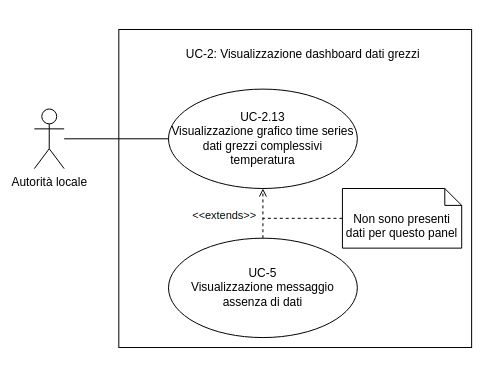
\includegraphics[width=0.5\textwidth]{analisi_dei_requisiti/UC-2.13.png}
	\captionof{figure}{UC-2.13: Visualizzazione grafico \href{https://7last.github.io/docs/pb/documentazione-interna/glossario\#time-series}{time series\textsubscript{G}} dati grezzi complessivi temperatura}
\end{center}

\newpage
\subsubsubsection{UC-2.14: Visualizzazione grafico time series dati grezzi complessivi umidità}
\begin{itemize}
	\item \textbf{Attore principale}: autorità locale.
	\item \textbf{Precondizioni}: l'autorità locale ha effettuato l'accesso al sistema ed esso è in funzione.
	\item \textbf{Postcondizioni}: l'autorità locale visualizza un grafico \href{https://7last.github.io/docs/pb/documentazione-interna/glossario\#time-series}{time series\textsubscript{G}} contenente i dati grezzi di umidità trasmessi da tutti i sensori presenti nella città, mostrando sull'asse delle ascisse i timestamp delle misurazioni e su quello delle ordinate i valori delle misurazioni di umidità in percentuale.
	\item \textbf{Scenario principale}:
	      \begin{enumerate}
		      \item l'autorità locale accede alla piattaforma;
		      \item il sistema carica i dati trasmessi dai sensori interrogando il database;
		      \item l'autorità locale seleziona la visualizzazione della \href{https://7last.github.io/docs/pb/documentazione-interna/glossario\#dashboard}{dashboard\textsubscript{G}} dei dati grezzi.
	      \end{enumerate}
	\item \href{https://7last.github.io/docs/pb/documentazione-interna/glossario\#user-story}{\textbf{User story}\textsubscript{G}}:
	      come autorità locale desidero poter visualizzare un grafico \href{https://7last.github.io/docs/pb/documentazione-interna/glossario\#time-series}{time series\textsubscript{G}} contenente i dati grezzi trasmessi da tutti i sensori
	      di umidità presenti nella città, espressi in percentuale, in modo da poterli confrontare tra loro e analizzare in modo più dettagliato.
\end{itemize}
\begin{center}
	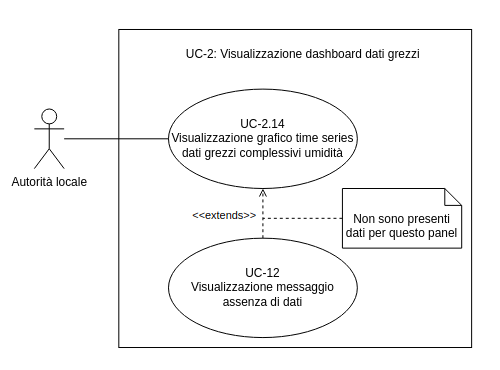
\includegraphics[width=0.5\textwidth]{analisi_dei_requisiti/UC-2.14.png}
	\captionof{figure}{UC-2.14: Visualizzazione grafico \href{https://7last.github.io/docs/pb/documentazione-interna/glossario\#time-series}{time series\textsubscript{G}} dati grezzi complessivi umidità}
\end{center}

\newpage
\subsubsubsection{UC-2.15: Visualizzazione grafico time series dati grezzi complessivi traffico}
\begin{itemize}
	\item \textbf{Attore principale}: autorità locale.
	\item \textbf{Precondizioni}: l'autorità locale ha effettuato l'accesso al sistema ed esso è in funzione.
	\item \textbf{Postcondizioni}: l'autorità locale visualizza un grafico \href{https://7last.github.io/docs/pb/documentazione-interna/glossario\#time-series}{time series\textsubscript{G}} contenente i dati grezzi di traffico trasmessi da tutti i sensori presenti nella città, mostrando sull'asse delle ascisse i timestamp delle misurazioni e su quello delle ordinate i valori delle misurazioni del numero di veicoli transitati.
	\item \textbf{Scenario principale}:
	      \begin{enumerate}
		      \item l'autorità locale accede alla piattaforma;
		      \item il sistema carica i dati trasmessi dai sensori interrogando il database;
		      \item l'autorità locale seleziona la visualizzazione della \href{https://7last.github.io/docs/pb/documentazione-interna/glossario\#dashboard}{dashboard\textsubscript{G}} dei dati grezzi.
	      \end{enumerate}
	\item \href{https://7last.github.io/docs/pb/documentazione-interna/glossario\#user-story}{\textbf{User story}\textsubscript{G}}:
	      come autorità locale desidero poter visualizzare un grafico \href{https://7last.github.io/docs/pb/documentazione-interna/glossario\#time-series}{time series\textsubscript{G}} contenente i dati grezzi del numero di veicoli transitati rilevati dai sensori di traffico.
\end{itemize}
\begin{center}
	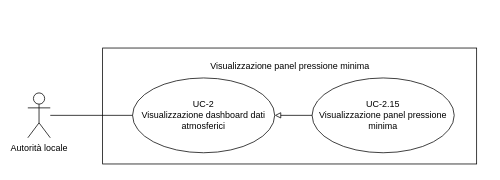
\includegraphics[width=0.5\textwidth]{analisi_dei_requisiti/UC-2.15.png}
	\captionof{figure}{UC-2.15: Visualizzazione grafico \href{https://7last.github.io/docs/pb/documentazione-interna/glossario\#time-series}{time series\textsubscript{G}} dati grezzi complessivi traffico}
\end{center}

\newpage
\subsubsubsection{UC-2.16: Visualizzazione grafico time series dati grezzi complessivi qualità dell'aria}
\begin{itemize}
	\item \textbf{Attore principale}: autorità locale.
	\item \textbf{Precondizioni}: l'autorità locale ha effettuato l'accesso al sistema ed esso è in funzione.
	\item \textbf{Postcondizioni}: l'autorità locale visualizza un grafico \href{https://7last.github.io/docs/pb/documentazione-interna/glossario\#time-series}{time series\textsubscript{G}} contenente i dati grezzi trasmessi da tutti i sensori di qualità dell'aria presenti nella città, mostrando sull'asse delle ascisse i timestamp delle misurazioni e su quello delle ordinate i valori delle misurazioni dei valori di PM10, PM2.5, NO\textsubscript{2}, O\textsubscript{3} e SO\textsubscript{2}. 
	\item \textbf{Scenario principale}:
	      \begin{enumerate}
		      \item l'autorità locale accede alla piattaforma;
		      \item il sistema carica i dati trasmessi dai sensori interrogando il database;
		      \item l'autorità locale seleziona la visualizzazione della \href{https://7last.github.io/docs/pb/documentazione-interna/glossario\#dashboard}{dashboard\textsubscript{G}} dei dati grezzi.
	      \end{enumerate}
	\item \href{https://7last.github.io/docs/pb/documentazione-interna/glossario\#user-story}{\textbf{User story}\textsubscript{G}}:
	      come autorità locale desidero poter visualizzare un grafico \href{https://7last.github.io/docs/pb/documentazione-interna/glossario\#time-series}{time series\textsubscript{G}} contenente le misurazioni di PM10, PM2.5, NO\textsubscript{2}, O\textsubscript{3}, SO\textsubscript{2} rilevatate dai sensori di qualità dell'aria, in modo da poterli confrontare tra loro e analizzare in modo più dettagliato.
\end{itemize}
\begin{center}
	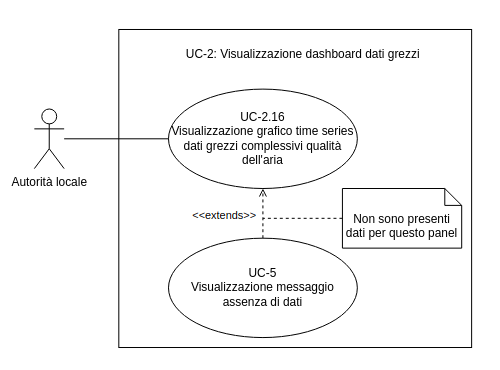
\includegraphics[width=0.5\textwidth]{analisi_dei_requisiti/UC-2.16.png}
	\captionof{figure}{UC-2.16: Visualizzazione grafico \href{https://7last.github.io/docs/pb/documentazione-interna/glossario\#time-series}{time series\textsubscript{G}} dati grezzi complessivi qualità dell'aria}
\end{center}

\newpage
\subsubsubsection{UC-2.17: Visualizzazione grafico time series dati grezzi complessivi precipitazioni}
\begin{itemize}
	\item \textbf{Attore principale}: autorità locale.
	\item \textbf{Precondizioni}: l'autorità locale ha effettuato l'accesso al sistema ed esso è in funzione.
	\item \textbf{Postcondizioni}: l'autorità locale visualizza un grafico \href{https://7last.github.io/docs/pb/documentazione-interna/glossario\#time-series}{time series\textsubscript{G}} contenente i dati grezzi trasmessi da tutti i sensori di precipitazioni presenti nella città, mostrando sull'asse delle ascisse i timestamp delle misurazioni e su quello delle ordinate i valori delle misurazioni delle precipitazioni espresse in millimetri.
	\item \textbf{Scenario principale}:
	      \begin{enumerate}
		      \item l'autorità locale accede alla piattaforma;
		      \item il sistema carica i dati trasmessi dai sensori interrogando il database;
		      \item l'autorità locale seleziona la visualizzazione della \href{https://7last.github.io/docs/pb/documentazione-interna/glossario\#dashboard}{dashboard\textsubscript{G}} dei dati grezzi.
	      \end{enumerate}
	\item \href{https://7last.github.io/docs/pb/documentazione-interna/glossario\#user-story}{\textbf{User story}\textsubscript{G}}:
	      come autorità locale desidero poter visualizzare un grafico \href{https://7last.github.io/docs/pb/documentazione-interna/glossario\#time-series}{time series\textsubscript{G}} contenente le misurazioni in millimetri rilevate dai sensori
	      di precipitazioni presenti nella città, in modo da poterli confrontare tra loro e analizzare in modo più dettagliato.
\end{itemize}
\begin{center}
	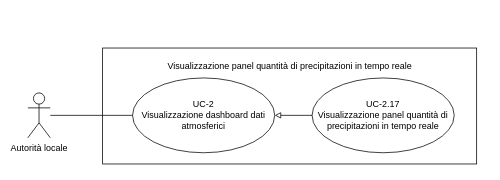
\includegraphics[width=0.5\textwidth]{analisi_dei_requisiti/UC-2.17.png}
	\captionof{figure}{UC-2.17: Visualizzazione grafico \href{https://7last.github.io/docs/pb/documentazione-interna/glossario\#time-series}{time series\textsubscript{G}} dati grezzi complessivi precipitazioni}
\end{center}

\newpage
\subsubsubsection{UC-2.18: Visualizzazione grafico time series dati grezzi complessivi isole ecologiche}
\begin{itemize}
	\item \textbf{Attore principale}: autorità locale.
	\item \textbf{Precondizioni}: l'autorità locale ha effettuato l'accesso al sistema ed esso è in funzione.
	\item \textbf{Postcondizioni}: l'autorità locale visualizza un grafico \href{https://7last.github.io/docs/pb/documentazione-interna/glossario\#time-series}{time series\textsubscript{G}} contenente i dati grezzi trasmessi da tutti i sensori di isole ecologiche presenti nella città, mostrando sull'asse delle ascisse i timestamp delle misurazioni e su quello delle ordinate i valori delle misurazioni del riempimento in percentuale.
	\item \textbf{Scenario principale}:
	      \begin{enumerate}
		      \item l'autorità locale accede alla piattaforma;
		      \item il sistema carica i dati trasmessi dai sensori interrogando il database;
		      \item l'autorità locale seleziona la visualizzazione della \href{https://7last.github.io/docs/pb/documentazione-interna/glossario\#dashboard}{dashboard\textsubscript{G}} dei dati grezzi.
	      \end{enumerate}
	\item \href{https://7last.github.io/docs/pb/documentazione-interna/glossario\#user-story}{\textbf{User story}\textsubscript{G}}:
	      come autorità locale desidero poter visualizzare un grafico \href{https://7last.github.io/docs/pb/documentazione-interna/glossario\#time-series}{time series\textsubscript{G}} contenente lo storico delle misurazioni del riempimento in percentuale
	      dei sensori di isole, in modo da poterli confrontare tra loro e analizzare in modo più dettagliato.
\end{itemize}
\begin{center}
	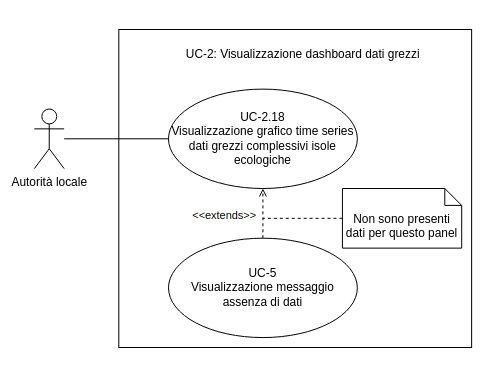
\includegraphics[width=0.5\textwidth]{analisi_dei_requisiti/UC-2.18.png}
	\captionof{figure}{UC-2.18: Visualizzazione grafico \href{https://7last.github.io/docs/pb/documentazione-interna/glossario\#time-series}{time series\textsubscript{G}} dati grezzi complessivi isole ecologiche}
\end{center}

\newpage
\subsubsubsection{UC-2.19: Visualizzazione grafico time series dati grezzi complessivi livello dei fiumi}
\begin{itemize}
	\item \textbf{Attore principale}: autorità locale.
	\item \textbf{Precondizioni}: l'autorità locale ha effettuato l'accesso al sistema ed esso è in funzione.
	\item \textbf{Postcondizioni}: l'autorità locale visualizza un grafico \href{https://7last.github.io/docs/pb/documentazione-interna/glossario\#time-series}{time series\textsubscript{G}} contenente i dati grezzi trasmessi da tutti i sensori di livello dei fiumi presenti nella città, mostrando sull'asse delle ascisse i timestamp delle misurazioni e su quello delle ordinate i valori delle misurazioni del livello dei fiumi in metri.
	\item \textbf{Scenario principale}:
	      \begin{enumerate}
		      \item l'autorità locale accede alla piattaforma;
		      \item il sistema carica i dati trasmessi dai sensori interrogando il database;
		      \item l'autorità locale seleziona la visualizzazione della \href{https://7last.github.io/docs/pb/documentazione-interna/glossario\#dashboard}{dashboard\textsubscript{G}} dei dati grezzi.
	      \end{enumerate}
	\item \href{https://7last.github.io/docs/pb/documentazione-interna/glossario\#user-story}{\textbf{User story}\textsubscript{G}}:
	      come autorità locale desidero poter visualizzare un grafico \href{https://7last.github.io/docs/pb/documentazione-interna/glossario\#time-series}{time series\textsubscript{G}} contenente le misurazioni in metri di acqua rilevate dai sensori
	      di livello dei fiumi presenti nella città, in modo da poterli confrontare tra loro e analizzare in modo più dettagliato.
\end{itemize}
\begin{center}
	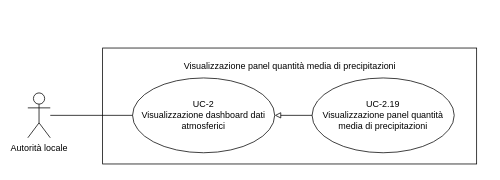
\includegraphics[width=0.5\textwidth]{analisi_dei_requisiti/UC-2.19.png}
	\captionof{figure}{UC-2.19: Visualizzazione grafico \href{https://7last.github.io/docs/pb/documentazione-interna/glossario\#time-series}{time series\textsubscript{G}} dati grezzi complessivi livello dei fiumi}
\end{center}

\newpage
\subsubsubsection{UC-2.20: Visualizzazione grafico time series dati grezzi complessivi colonnine di ricarica}
\begin{itemize}
	\item \textbf{Attore principale}: autorità locale.
	\item \textbf{Precondizioni}: l'autorità locale ha effettuato l'accesso al sistema ed esso è in funzione.
	\item \textbf{Postcondizioni}: l'autorità locale visualizza un grafico \href{https://7last.github.io/docs/pb/documentazione-interna/glossario\#time-series}{time series\textsubscript{G}} contenente i dati grezzi trasmessi da tutti i sensori di colonnine di ricarica presenti nella città, mostrando sull'asse delle ascisse i timestamp delle misurazioni e su quello delle ordinate i valori delle misurazioni della potenza erogata in kWh.
	\item \textbf{Scenario principale}:
	      \begin{enumerate}
		      \item l'autorità locale accede alla piattaforma;
		      \item il sistema carica i dati trasmessi dai sensori interrogando il database;
		      \item l'autorità locale seleziona la visualizzazione della \href{https://7last.github.io/docs/pb/documentazione-interna/glossario\#dashboard}{dashboard\textsubscript{G}} dei dati grezzi.
	      \end{enumerate}
	\item \href{https://7last.github.io/docs/pb/documentazione-interna/glossario\#user-story}{\textbf{User story}\textsubscript{G}}:
	      come autorità locale desidero poter visualizzare un grafico \href{https://7last.github.io/docs/pb/documentazione-interna/glossario\#time-series}{time series\textsubscript{G}} contenente le misurazioni in kWh della potenza erogata
	      e il tempo rimanente alla ricarica rilevati dalle colonnine di ricarica.
\end{itemize}
\begin{center}
	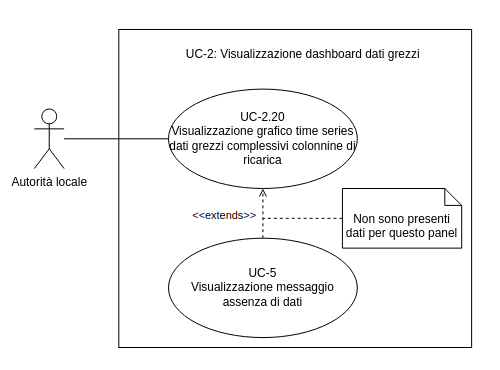
\includegraphics[width=0.5\textwidth]{analisi_dei_requisiti/UC-2.20.png}
	\captionof{figure}{UC-2.20: Visualizzazione grafico \href{https://7last.github.io/docs/pb/documentazione-interna/glossario\#time-series}{time series\textsubscript{G}} dati grezzi complessivi colonnine di ricarica}
\end{center}


%%%%%%%%%%%%%%%%%%%%%%%%%%%%%%%%%%%%%%%%%%INIZIO AMBIENTALI%%%%%%%%%%%%%%%%%%%%%%%%%%%%%%%%%%%%%%%%

\newpage
\subsubsection{UC-3: Visualizzazione dashboard dati ambientali}
\begin{itemize}
	\item \textbf{Attore principale}: autorità locale.
	\item \textbf{Precondizioni}: l'autorità locale ha effettuato l'accesso al sistema ed esso è in funzione.
	\item \textbf{Postcondizioni}: l'autorità locale visualizza la \href{https://7last.github.io/docs/pb/documentazione-interna/glossario\#dashboard}{dashboard\textsubscript{G}} contenente le sezioni relative ai sensori ambientali presenti nella città ovvero temperatura, umidità, precipitazioni, livello dei fiumi e qualità dell'aria.
	\item \textbf{Scenario principale}:
	      \begin{enumerate}
		      \item l'autorità locale accede alla piattaforma;
		      \item il sistema carica i dati relativi ai sensori interrogando il database.
	      \end{enumerate}
	\item \href{https://7last.github.io/docs/pb/documentazione-interna/glossario\#user-story}{\textbf{User story}\textsubscript{G}}: come autorità locale desidero poter visualizzare una \href{https://7last.github.io/docs/pb/documentazione-interna/glossario\#dashboard}{dashboard\textsubscript{G}} dei dati ambientali, la quale mi consente di visualizzare le sezioni relative ai sensori ambientali presenti nella città, ovvero temperatura, umidità, precipitazioni, livello dei fiumi e qualità dell'aria.
\end{itemize}
\begin{center}
	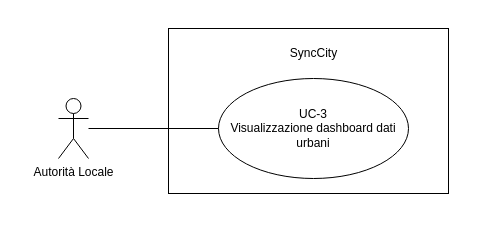
\includegraphics[width=0.5\textwidth]{analisi_dei_requisiti/UC-3.png}
	\captionof{figure}{UC-3: Visualizzazione \href{https://7last.github.io/docs/pb/documentazione-interna/glossario\#dashboard}{dashboard\textsubscript{G}} dei dati ambientali}
\end{center}

\newpage
\subsubsubsection{UC-3.1: Visualizzazione sezione temperatura}
\begin{itemize}
	\item \textbf{Attore principale}: autorità locale.
	\item \textbf{Precondizioni}: l'autorità locale ha effettuato l'accesso al sistema ed esso è in funzione.
	\item \textbf{Postcondizioni}: l'autorità locale visualizza la sezione relativa ai sensori di temperatura presenti nella città, la quale contiene un grafico time series con le misurazioni storiche della temperatura, una mappa dei sensori di temperatura collegati al sistema, dei panel che mostrano la temperatura media, massima e minima nel periodo di tempo selezionato e quella attuale e un panel con il valore di \textit{current year livability temperature index} medio nell'anno in corso.
	\item \textbf{Scenario principale}:
	      \begin{enumerate}
		      \item l'autorità locale accede alla piattaforma;
		      \item il sistema carica i dati trasmessi dai sensori interrogando il database;
		      \item l'autorità locale seleziona la visualizzazione della \href{https://7last.github.io/docs/pb/documentazione-interna/glossario\#dashboard}{dashboard\textsubscript{G}} relativa ai sensori ambientali.
	      \end{enumerate}
	\item \href{https://7last.github.io/docs/pb/documentazione-interna/glossario\#user-story}{\textbf{User story}\textsubscript{G}}:
	      come autorità locale desidero poter visualizzare una sezione relativa ai sensori di temperatura presenti nella città, la quale
	      conterrà un grafico time series con le misurazioni storiche della temperatura, una mappa dei sensori di temperatura collegati al sistema, dei panel che mostrano la temperatura media, massima e minima nel periodo di tempo selezionato e quella attuale e un panel con il valore di \textit{current year livability temperature index} medio nell'anno in corso.
\end{itemize}
\begin{center}
	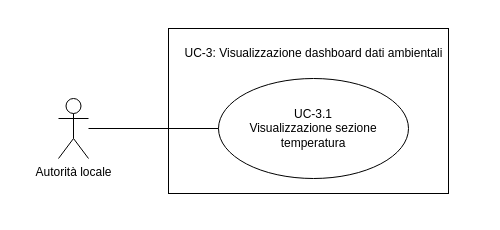
\includegraphics[width=0.5\textwidth]{analisi_dei_requisiti/UC-3.1.png}
	\captionof{figure}{UC-3.1: Visualizzazione sezione temperatura}
\end{center}

\newpage
\subsubsubsubsection{UC-3.1.1: Visualizzazione grafico time series temperatura}
\begin{itemize}
	\item \textbf{Attore principale}: autorità locale.
	\item \textbf{Precondizioni}:
	      \begin{enumerate}
		      \item l'autorità locale ha effettuato l'accesso al sistema ed esso è in funzione;
		      \item il sistema ha caricato la \href{https://7last.github.io/docs/pb/documentazione-interna/glossario\#dashboard}{dashboard\textsubscript{G}} relativa ai sensori ambientali.
	      \end{enumerate}
	\item \textbf{Postcondizioni}: l'autorità locale visualizza un grafico \href{https://7last.github.io/docs/pb/documentazione-interna/glossario\#time-series}{time series\textsubscript{G}} contenente le misurazioni storiche della temperatura effettiva e percepita, ciascuna aggregata per 5 minuti.
	\item \textbf{Scenario principale}:
	      \begin{enumerate}
		      \item l'autorità locale accede alla piattaforma;
		      \item il sistema carica i dati relativi ai sensori interrogando il database;
		      \item l'autorità locale seleziona la visualizzazione della \href{https://7last.github.io/docs/pb/documentazione-interna/glossario\#dashboard}{dashboard\textsubscript{G}} relativa ai sensori ambientali.
	      \end{enumerate}
	\item \href{https://7last.github.io/docs/pb/documentazione-interna/glossario\#user-story}{\textbf{User story}\textsubscript{G}}: come autorità locale desidero poter visualizzare un grafico \href{https://7last.github.io/docs/pb/documentazione-interna/glossario\#time-series}{time series\textsubscript{G}} contenente le misurazioni storiche della temperatura effettiva e percepita per poterne monitorare l'andamento nel tempo e facilmente individuare eventuali anomalie.
\end{itemize}
\begin{center}
	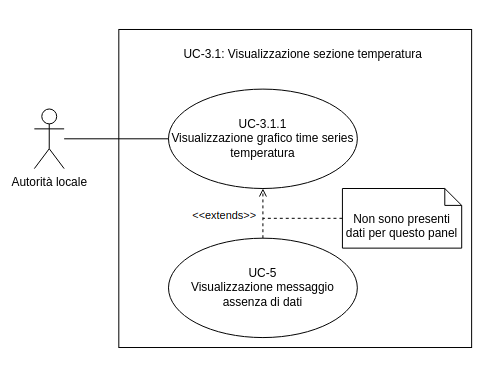
\includegraphics[width=0.5\textwidth]{analisi_dei_requisiti/UC-3.1.1.png}
	\captionof{figure}{UC-3.1.1: Visualizzazione grafico \href{https://7last.github.io/docs/pb/documentazione-interna/glossario\#time-series}{time series\textsubscript{G}} per temperatura}
\end{center}

\newpage
\subsubsubsubsection{UC-3.1.2: Visualizzazione mappa sensori temperatura}
\begin{itemize}
	\item \textbf{Attore principale}: autorità locale.
	\item \textbf{Precondizioni}:
	      \begin{enumerate}
		      \item l'autorità locale ha effettuato l'accesso al sistema ed esso è in funzione;
		      \item il sistema ha caricato la \href{https://7last.github.io/docs/pb/documentazione-interna/glossario\#dashboard}{dashboard\textsubscript{G}} relativa ai sensori ambientali.
	      \end{enumerate}
	\item \textbf{Postcondizioni}: l'autorità locale visualizza una mappa interattiva popolata con dei \textit{marker} contenenti l'identificativo e le coordinate geografiche dei sensori di temperatura, mostrando sia la temperatura misurata che quella percepita misurate in gradi Celsius.
	\item \textbf{Scenario principale}:
	      \begin{enumerate}
		      \item l'autorità locale accede alla piattaforma;
		      \item il sistema carica i dati relativi ai sensori interrogando il database;
		      \item l'autorità locale seleziona la visualizzazione della \href{https://7last.github.io/docs/pb/documentazione-interna/glossario\#dashboard}{dashboard\textsubscript{G}} relativa ai sensori ambientali.
	      \end{enumerate}
	\item \href{https://7last.github.io/docs/pb/documentazione-interna/glossario\#user-story}{\textbf{User story}\textsubscript{G}}:
	      come autorità locale desidero poter visualizzare una mappa interattiva popolata con dei \textit{marker} rappresentanti la posizione dei sensori di temperatura e contenenti il loro identificativo, mostrando anche la temperatura misurata e quella percepita misurate in gradi Celsius. Essa mi consentirà di visualizzare la distribuzione dei sensori di temperatura nel territorio ed eventualmente intervenire nel caso in cui siano presenti zone non coperte.
\end{itemize}
\begin{center}
	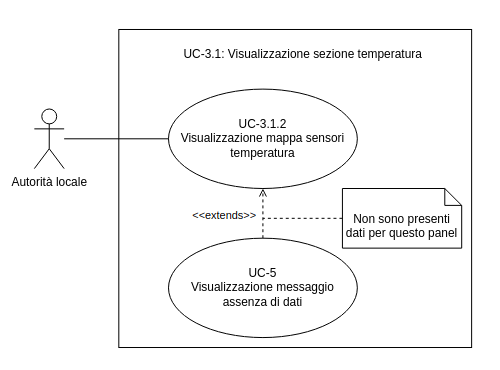
\includegraphics[width=0.5\textwidth]{analisi_dei_requisiti/UC-3.1.2.png}
	\captionof{figure}{UC-3.1.2: Visualizzazione mappa interattiva sensori temperatura}
\end{center}

\newpage
\subsubsubsubsection{UC-3.1.3: Visualizzazione \textit{panel} temperatura media nel periodo di tempo selezionato}
\begin{itemize}
	\item \textbf{Attore principale}: autorità locale.
	\item \textbf{Precondizioni}:
	      \begin{enumerate}
		      \item l'autorità locale ha effettuato l'accesso al sistema ed esso è in funzione;
		      \item il sistema ha caricato la \href{https://7last.github.io/docs/pb/documentazione-interna/glossario\#dashboard}{dashboard\textsubscript{G}} relativa ai sensori ambientali.
	      \end{enumerate}
	\item \textbf{Postcondizioni}: l'autorità locale visualizza un \href{https://7last.github.io/docs/pb/documentazione-interna/glossario\#panel}{\textit{panel}\textsubscript{G}} contenente la temperatura media nel periodo di tempo selezionato.
	\item \textbf{Scenario principale}:
	      \begin{enumerate}
		      \item l'autorità locale accede alla piattaforma;
		      \item il sistema carica i dati relativi ai sensori interrogando il database;
		      \item l'autorità locale seleziona la visualizzazione della \href{https://7last.github.io/docs/pb/documentazione-interna/glossario\#dashboard}{dashboard\textsubscript{G}} relativa ai sensori ambientali.
	      \end{enumerate}
	\item \href{https://7last.github.io/docs/pb/documentazione-interna/glossario\#user-story}{\textbf{User story}\textsubscript{G}}: come autorità locale desidero poter visualizzare la temperatura media nel periodo di tempo selezionato
	      in modo da poterne monitorare l'andamento.
\end{itemize}
\begin{center}
	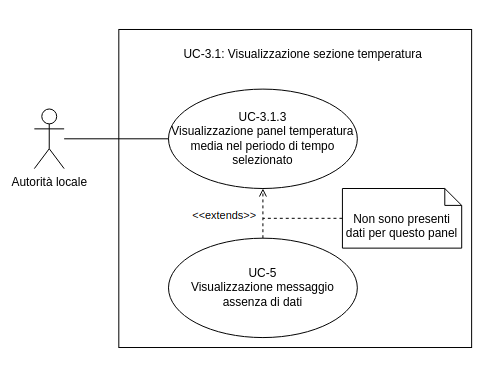
\includegraphics[width=0.5\textwidth]{analisi_dei_requisiti/UC-3.1.3.png}
	\captionof{figure}{UC-3.1.3: Visualizzazione \href{https://7last.github.io/docs/pb/documentazione-interna/glossario\#panel}{\textit{panel}\textsubscript{G}} temperatura media nel periodo di tempo selezionato}
\end{center}

\newpage
\subsubsubsubsection{UC-3.1.4: Visualizzazione gauge current year livability temperature index}
\begin{itemize}
	\item \textbf{Attore principale}: autorità locale.
	\item \textbf{Precondizioni}:
	      \begin{enumerate}
		      \item l'autorità locale ha effettuato l'accesso al sistema ed esso è in funzione;
		      \item il sistema ha caricato la \href{https://7last.github.io/docs/pb/documentazione-interna/glossario\#dashboard}{dashboard\textsubscript{G}} relativa ai sensori di temperatura.
	      \end{enumerate}
	\item \textbf{Postcondizioni}: l'autorità locale visualizza un gauge contenente il valore di \textit{current year livability temperature index} (CYLTI) nell'anno in corso, che rappresenta quanto sia confortevole la temperatura per l'essere umano.
	\item \textbf{Scenario principale}:
	      \begin{enumerate}
		      \item l'autorità locale accede alla piattaforma;
		      \item il sistema carica i dati relativi ai sensori interrogando il database;
		      \item l'autorità locale seleziona la visualizzazione della \href{https://7last.github.io/docs/pb/documentazione-interna/glossario\#dashboard}{dashboard\textsubscript{G}} relativa ai sensori di temperatura.
	      \end{enumerate}
	\item \href{https://7last.github.io/docs/pb/documentazione-interna/glossario\#user-story}{\textbf{User story}\textsubscript{G}}:
	      come autorità locale desidero poter visualizzare il valore di \textit{current year livability temperature index} nell'anno in corso.
\end{itemize}
\begin{center}
	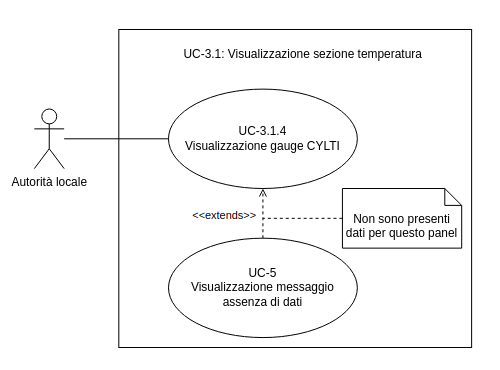
\includegraphics[width=0.5\textwidth]{analisi_dei_requisiti/UC-3.1.4.png}
	\captionof{figure}{UC-3.1.4: Visualizzazione \href{https://7last.github.io/docs/pb/documentazione-interna/glossario\#panel}{\textit{panel}\textsubscript{G}} temperatura in tempo reale}
\end{center}

\newpage
\subsubsubsubsection{UC-3.1.5: Visualizzazione \textit{panel} temperatura massima nel periodo di tempo selezionato}
\begin{itemize}
	\item \textbf{Attore principale}: autorità locale.
	\item \textbf{Precondizioni}:
	      \begin{enumerate}
		      \item l'autorità locale ha effettuato l'accesso al sistema ed esso è in funzione;
		      \item il sistema ha caricato la \href{https://7last.github.io/docs/pb/documentazione-interna/glossario\#dashboard}{dashboard\textsubscript{G}} relativa ai sensori ambientali.
	      \end{enumerate}
	\item \textbf{Postcondizioni}: l'autorità locale visualizza un \href{https://7last.github.io/docs/pb/documentazione-interna/glossario\#panel}{\textit{panel}\textsubscript{G}} contenente la temperatura massima nel periodo di tempo selezionato.
	\item \textbf{Scenario principale}:
	      \begin{enumerate}
		      \item l'autorità locale accede alla piattaforma;
		      \item il sistema carica i dati relativi ai sensori interrogando il database;
		      \item l'autorità locale seleziona la visualizzazione della \href{https://7last.github.io/docs/pb/documentazione-interna/glossario\#dashboard}{dashboard\textsubscript{G}} relativa ai sensori ambientali.
	      \end{enumerate}
	\item \href{https://7last.github.io/docs/pb/documentazione-interna/glossario\#user-story}{\textbf{User story}\textsubscript{G}}:
	      come autorità locale desidero poter visualizzare la temperatura massima nel periodo di tempo selezionato
	      in modo da poterla prendere come riferimento e confrontarla con la temperatura attuale.
\end{itemize}
\begin{center}
	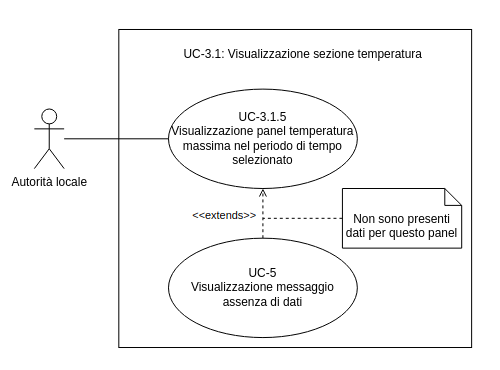
\includegraphics[width=0.5\textwidth]{analisi_dei_requisiti/UC-3.1.5.png}
	\captionof{figure}{UC-3.1.5: Visualizzazione \href{https://7last.github.io/docs/pb/documentazione-interna/glossario\#panel}{\textit{panel}\textsubscript{G}} temperatura massima}
\end{center}

\newpage
\subsubsubsubsection{UC-3.1.6: Visualizzazione \textit{panel} temperatura minima nel periodo di tempo selezionato}
\begin{itemize}
	\item \textbf{Attore principale}: autorità locale.
	\item \textbf{Precondizioni}:
	      \begin{enumerate}
		      \item l'autorità locale ha effettuato l'accesso al sistema ed esso è in funzione;
		      \item il sistema ha caricato la \href{https://7last.github.io/docs/pb/documentazione-interna/glossario\#dashboard}{dashboard\textsubscript{G}} relativa ai sensori ambientali.
	      \end{enumerate}
	\item \textbf{Postcondizioni}: l'autorità locale visualizza un \href{https://7last.github.io/docs/pb/documentazione-interna/glossario\#panel}{\textit{panel}\textsubscript{G}} contenente la temperatura minima nel periodo di tempo selezionato.
	\item \textbf{Scenario principale}:
	      \begin{enumerate}
		      \item l'autorità locale accede alla piattaforma;
		      \item il sistema carica i dati relativi ai sensori interrogando il database;
		      \item l'autorità locale seleziona la visualizzazione della \href{https://7last.github.io/docs/pb/documentazione-interna/glossario\#dashboard}{dashboard\textsubscript{G}} relativa ai sensori ambientali.
	      \end{enumerate}
	\item \href{https://7last.github.io/docs/pb/documentazione-interna/glossario\#user-story}{\textbf{User story}\textsubscript{G}}:
	      come autorità locale desidero poter visualizzare la temperatura minima nel periodo di tempo selezionato
	      in modo da poterla prendere come riferimento e confrontarla con la temperatura attuale.
\end{itemize}
\begin{center}
	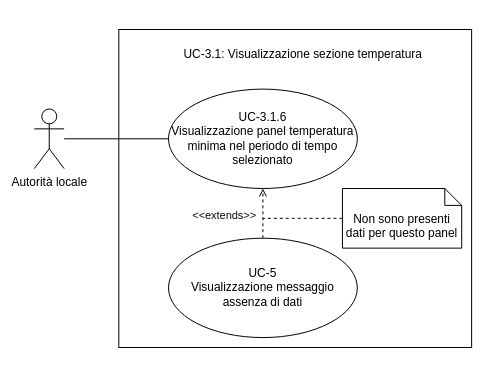
\includegraphics[width=0.5\textwidth]{analisi_dei_requisiti/UC-3.1.6.png}
	\captionof{figure}{UC-3.1.6: Visualizzazione \href{https://7last.github.io/docs/pb/documentazione-interna/glossario\#panel}{\textit{panel}\textsubscript{G}} temperatura minima}
\end{center}

\newpage
\subsubsubsection{UC-3.2: Visualizzazione sezione umidità}
\begin{itemize}
	\item \textbf{Attore principale}: autorità locale.
	\item \textbf{Precondizioni}: l'autorità locale ha effettuato l'accesso al sistema ed esso è in funzione.
	\item \textbf{Postcondizioni}: l'autorità locale visualizza la \href{https://7last.github.io/docs/pb/documentazione-interna/glossario\#dashboard}{dashboard\textsubscript{G}} relativa ai sensori ambientali presenti nella città, la quale contiene un grafico time series con le misurazioni storiche dell'umidità, una mappa dei sensori di umidità collegati al sistema, dei panel che mostrano l'umidità media, massima e minima nel periodo di tempo selezionato e quella attuale.
	\item \textbf{Scenario principale}:
	      \begin{enumerate}
		      \item l'autorità locale accede alla piattaforma;
		      \item il sistema carica i dati trasmessi dai sensori interrogando il database;
		      \item l'autorità locale seleziona la visualizzazione della \href{https://7last.github.io/docs/pb/documentazione-interna/glossario\#dashboard}{dashboard\textsubscript{G}} relativa ai ambientali.
	      \end{enumerate}
	\item \href{https://7last.github.io/docs/pb/documentazione-interna/glossario\#user-story}{\textbf{User story}\textsubscript{G}}:
	      come autorità locale desidero poter visualizzare una \href{https://7last.github.io/docs/pb/documentazione-interna/glossario\#dashboard}{dashboard\textsubscript{G}} relativa ai sensori di umidità presenti nella città, la quale conterrà un grafico time series con le misurazioni storiche dell'umidità, una mappa dei sensori di umidità collegati al sistema, dei panel che mostrano l'umidità media, massima e minima nel periodo di tempo selezionato e quella attuale.
\end{itemize}
\begin{center}
	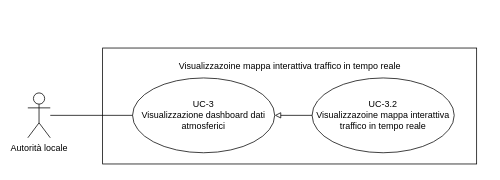
\includegraphics[width=0.5\textwidth]{analisi_dei_requisiti/UC-3.2.png}
	\captionof{figure}{UC-3.2: Visualizzazione sezione umidità}
\end{center}

\newpage
\subsubsubsubsection{UC-3.2.1: Visualizzazione grafico time series umidità}
\begin{itemize}
	\item \textbf{Attore principale}: autorità locale.
	\item \textbf{Precondizioni}:
	      \begin{enumerate}
		      \item l'autorità locale ha effettuato l'accesso al sistema ed esso è in funzione;
		      \item il sistema ha caricato la \href{https://7last.github.io/docs/pb/documentazione-interna/glossario\#dashboard}{dashboard\textsubscript{G}} relativa ai sensori ambientali.
	      \end{enumerate}
	\item \textbf{Postcondizioni}: l'autorità locale visualizza un grafico \href{https://7last.github.io/docs/pb/documentazione-interna/glossario\#time-series}{time series\textsubscript{G}} contenente le misurazioni storiche di umidità aggregate per 5 minuti.
	\item \textbf{Scenario principale}:
	      \begin{enumerate}
		      \item l'autorità locale accede alla piattaforma;
		      \item il sistema carica i dati relativi ai sensori interrogando il database;
		      \item l'autorità locale seleziona la visualizzazione della \href{https://7last.github.io/docs/pb/documentazione-interna/glossario\#dashboard}{dashboard\textsubscript{G}} relativa ai sensori ambientali.
	      \end{enumerate}
	\item \href{https://7last.github.io/docs/pb/documentazione-interna/glossario\#user-story}{\textbf{User story}\textsubscript{G}}:
	      come autorità locale desidero poter visualizzare un grafico \href{https://7last.github.io/docs/pb/documentazione-interna/glossario\#time-series}{time series\textsubscript{G}} contenente le misurazioni storiche
	      di umidità per poter monitorarne l'andamento nel tempo e facilmente individuare eventuali anomalie.
\end{itemize}
\begin{center}
	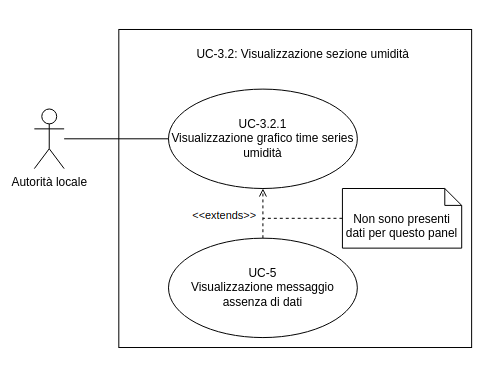
\includegraphics[width=0.5\textwidth]{analisi_dei_requisiti/UC-3.2.1.png}
	\captionof{figure}{UC-3.2.1: Visualizzazione grafico \href{https://7last.github.io/docs/pb/documentazione-interna/glossario\#time-series}{time series\textsubscript{G}} umidità}
\end{center}

\newpage
\subsubsubsubsection{UC-3.2.2: Visualizzazione mappa sensori umidità}
\begin{itemize}
	\item \textbf{Attore principale}: autorità locale.
	\item \textbf{Precondizioni}:
	      \begin{enumerate}
		      \item l'autorità locale ha effettuato l'accesso al sistema ed esso è in funzione;
		      \item il sistema ha caricato la \href{https://7last.github.io/docs/pb/documentazione-interna/glossario\#dashboard}{dashboard\textsubscript{G}} relativa ai sensori ambientali.
	      \end{enumerate}
	\item \textbf{Postcondizioni}: l'autorità locale visualizza una mappa interattiva popolata con dei \textit{marker} contenenti l'identificativo e le coordinate geografiche dei sensori di umidità.
	\item \textbf{Scenario principale}:
	      \begin{enumerate}
		      \item l'autorità locale accede alla piattaforma;
		      \item il sistema carica i dati relativi ai sensori interrogando il database;
		      \item l'autorità locale seleziona la visualizzazione della \href{https://7last.github.io/docs/pb/documentazione-interna/glossario\#dashboard}{dashboard\textsubscript{G}} relativa ai sensori ambientali.
	      \end{enumerate}
	\item \href{https://7last.github.io/docs/pb/documentazione-interna/glossario\#user-story}{\textbf{User story}\textsubscript{G}}:
	      come autorità locale desidero poter visualizzare una mappa interattiva popolata con dei \textit{marker} rappresentanti la posizione dei sensori di umidità
	      e contenenti il loro identificativo. Essa mi consentirà di visualizzare la distribuzione dei sensori di umidità nel territorio ed eventualmente intervenire nel caso in cui siano presenti zone non coperte.
\end{itemize}
\begin{center}
	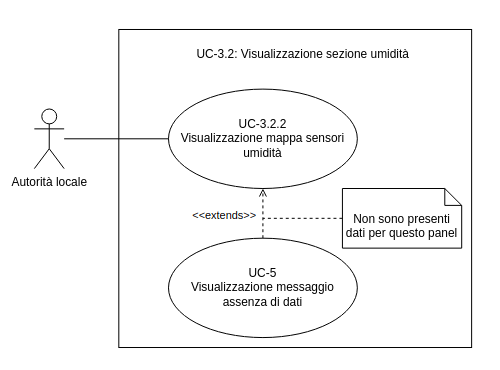
\includegraphics[width=0.5\textwidth]{analisi_dei_requisiti/UC-3.2.2.png}
	\captionof{figure}{UC-3.2.2: Visualizzazione mappa interattiva sensori umidità}
\end{center}

\newpage
\subsubsubsubsection{UC-3.2.3: Visualizzazione \textit{panel} umidità media nel periodo di tempo selezionato}
\begin{itemize}
	\item \textbf{Attore principale}: autorità locale.
	\item \textbf{Precondizioni}:
	      \begin{enumerate}
		      \item l'autorità locale ha effettuato l'accesso al sistema ed esso è in funzione;
		      \item il sistema ha caricato la \href{https://7last.github.io/docs/pb/documentazione-interna/glossario\#dashboard}{dashboard\textsubscript{G}} relativa ai sensori ambientali.
	      \end{enumerate}
	\item \textbf{Postcondizioni}: l'autorità locale visualizza un \href{https://7last.github.io/docs/pb/documentazione-interna/glossario\#panel}{\textit{panel}\textsubscript{G}} contenente l'umidità media nel periodo di tempo selezionato.
	\item \textbf{Scenario principale}:
	      \begin{enumerate}
		      \item l'autorità locale accede alla piattaforma;
		      \item il sistema carica i dati relativi ai sensori interrogando il database;
		      \item l'autorità locale seleziona la visualizzazione della \href{https://7last.github.io/docs/pb/documentazione-interna/glossario\#dashboard}{dashboard\textsubscript{G}} relativa ai sensori ambientali.
	      \end{enumerate}
	\item \href{https://7last.github.io/docs/pb/documentazione-interna/glossario\#user-story}{\textbf{User story}\textsubscript{G}}: come autorità locale desidero poter visualizzare l'umidità media nel periodo di tempo selezionato
	      in modo da poterne monitorare l'andamento.
\end{itemize}
\begin{center}
	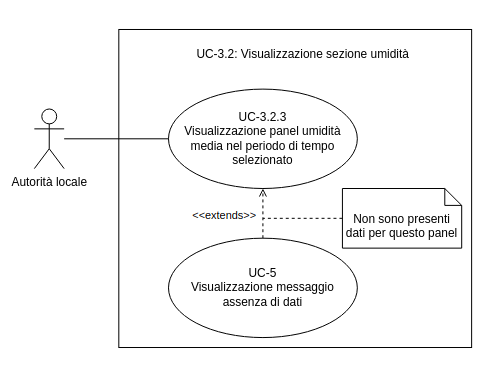
\includegraphics[width=0.5\textwidth]{analisi_dei_requisiti/UC-3.2.3.png}
	\captionof{figure}{UC-3.2.3: Visualizzazione \href{https://7last.github.io/docs/pb/documentazione-interna/glossario\#panel}{\textit{panel}\textsubscript{G}} umidità media nel periodo di tempo selezionato}
\end{center}

\newpage
\subsubsubsubsection{UC-3.2.4: Visualizzazione \textit{panel} umidità in tempo reale}
\begin{itemize}
	\item \textbf{Attore principale}: autorità locale.
	\item \textbf{Precondizioni}:
	      \begin{enumerate}
		      \item l'autorità locale ha effettuato l'accesso al sistema ed esso è in funzione;
		      \item il sistema ha caricato la \href{https://7last.github.io/docs/pb/documentazione-interna/glossario\#dashboard}{dashboard\textsubscript{G}} relativa ai sensori ambientali.
	      \end{enumerate}
	\item \textbf{Postcondizioni}: l'autorità locale visualizza un \href{https://7last.github.io/docs/pb/documentazione-interna/glossario\#panel}{\textit{panel}\textsubscript{G}} contenente l'umidità in tempo reale.
	\item \textbf{Scenario principale}:
	      \begin{enumerate}
		      \item l'autorità locale accede alla piattaforma;
		      \item il sistema carica i dati relativi ai sensori interrogando il database;
		      \item l'autorità locale seleziona la visualizzazione della \href{https://7last.github.io/docs/pb/documentazione-interna/glossario\#dashboard}{dashboard\textsubscript{G}} relativa ai sensori ambientali.
	      \end{enumerate}
	\item \href{https://7last.github.io/docs/pb/documentazione-interna/glossario\#user-story}{\textbf{User story}\textsubscript{G}}:
	      come autorità locale desidero poter visualizzare l'umidità in tempo reale in modo da poterne monitorare l'andamento
	      e poterla facilmente confrontare con i dati storici.
\end{itemize}
\begin{center}
	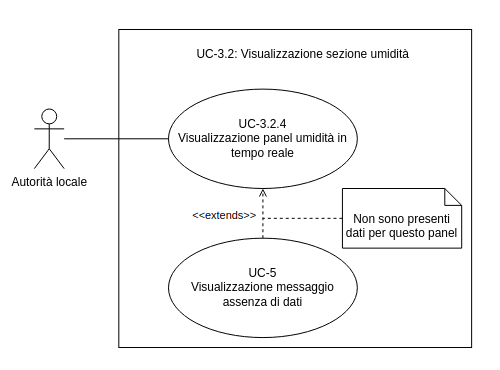
\includegraphics[width=0.5\textwidth]{analisi_dei_requisiti/UC-3.2.4.png}
	\captionof{figure}{UC-3.2.4: Visualizzazione \href{https://7last.github.io/docs/pb/documentazione-interna/glossario\#panel}{\textit{panel}\textsubscript{G}} umidità in tempo reale}
\end{center}

\newpage
\subsubsubsubsection{UC-3.2.5: Visualizzazione \textit{panel} umidità massima nel periodo di tempo selezionato}
\begin{itemize}
	\item \textbf{Attore principale}: autorità locale.
	\item \textbf{Precondizioni}:
	      \begin{enumerate}
		      \item l'autorità locale ha effettuato l'accesso al sistema ed esso è in funzione;
		      \item il sistema ha caricato la \href{https://7last.github.io/docs/pb/documentazione-interna/glossario\#dashboard}{dashboard\textsubscript{G}} relativa ai sensori ambientali.
	      \end{enumerate}
	\item \textbf{Postcondizioni}: l'autorità locale visualizza un \href{https://7last.github.io/docs/pb/documentazione-interna/glossario\#panel}{\textit{panel}\textsubscript{G}} contenente l'umidità massima nel periodo di tempo selezionato.
	\item \textbf{Scenario principale}:
	      \begin{enumerate}
		      \item l'autorità locale accede alla piattaforma;
		      \item il sistema carica i dati relativi ai sensori interrogando il database;
		      \item l'autorità locale seleziona la visualizzazione della \href{https://7last.github.io/docs/pb/documentazione-interna/glossario\#dashboard}{dashboard\textsubscript{G}} relativa ai sensori ambientali.
	      \end{enumerate}
	\item \href{https://7last.github.io/docs/pb/documentazione-interna/glossario\#user-story}{\textbf{User story}\textsubscript{G}}:
	      come autorità locale desidero poter visualizzare l'umidità massima nel periodo di tempo selezionato
	      in modo da poterla prendere come riferimento e confrontarla con l'umidità attuale.
\end{itemize}
\begin{center}
	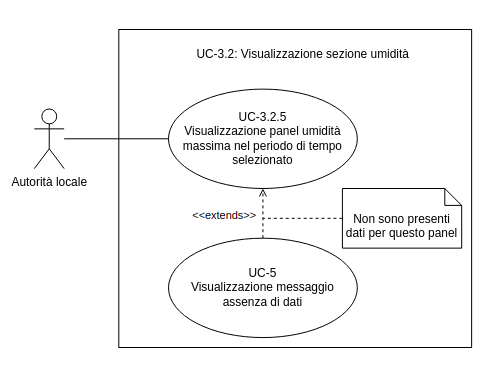
\includegraphics[width=0.5\textwidth]{analisi_dei_requisiti/UC-3.2.5.png}
	\captionof{figure}{UC-3.2.5: Visualizzazione \href{https://7last.github.io/docs/pb/documentazione-interna/glossario\#panel}{\textit{panel}\textsubscript{G}} umidità massima}
\end{center}

\newpage
\subsubsubsubsection{UC-3.2.6: Visualizzazione \textit{panel} umidità minima nel periodo di tempo selezionato}
\begin{itemize}
	\item \textbf{Attore principale}: autorità locale.
	\item \textbf{Precondizioni}:
	      \begin{enumerate}
		      \item l'autorità locale ha effettuato l'accesso al sistema ed esso è in funzione;
		      \item il sistema ha caricato la \href{https://7last.github.io/docs/pb/documentazione-interna/glossario\#dashboard}{dashboard\textsubscript{G}} relativa ai sensori ambientali.
	      \end{enumerate}
	\item \textbf{Postcondizioni}: l'autorità locale visualizza un \href{https://7last.github.io/docs/pb/documentazione-interna/glossario\#panel}{\textit{panel}\textsubscript{G}} contenente l'umidità minima nel periodo di tempo selezionato.
	\item \textbf{Scenario principale}:
	      \begin{enumerate}
		      \item l'autorità locale accede alla piattaforma;
		      \item il sistema carica i dati relativi ai sensori interrogando il database;
		      \item l'autorità locale seleziona la visualizzazione della \href{https://7last.github.io/docs/pb/documentazione-interna/glossario\#dashboard}{dashboard\textsubscript{G}} relativa ai sensori ambientali.
	      \end{enumerate}
	\item \href{https://7last.github.io/docs/pb/documentazione-interna/glossario\#user-story}{\textbf{User story}\textsubscript{G}}:
	      come autorità locale desidero poter visualizzare l'umidità minima nel periodo di tempo selezionato
	      in modo da poterla prendere come riferimento e confrontarla con l'umidità attuale.
\end{itemize}
\begin{center}
	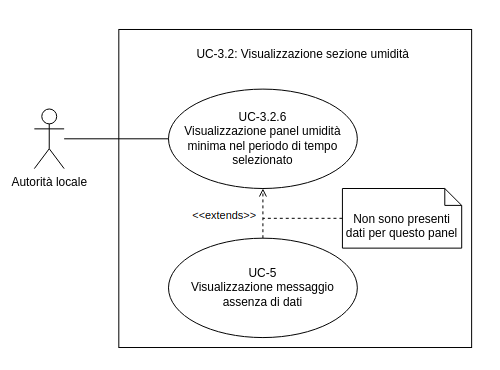
\includegraphics[width=0.5\textwidth]{analisi_dei_requisiti/UC-3.2.6.png}
	\captionof{figure}{UC-3.2.6: Visualizzazione \href{https://7last.github.io/docs/pb/documentazione-interna/glossario\#panel}{\textit{panel}\textsubscript{G}} umidità minima}
\end{center}

\newpage
\subsubsubsection{UC-3.3: Visualizzazione sezione qualità dell'aria}
\begin{itemize}
	\item \textbf{Attore principale}: autorità locale.
	\item \textbf{Precondizioni}: l'autorità locale ha effettuato l'accesso al sistema ed esso è in funzione.
	\item \textbf{Postcondizioni}: l'autorità locale visualizza la \href{https://7last.github.io/docs/pb/documentazione-interna/glossario\#dashboard}{dashboard\textsubscript{G}} relativa ai sensori ambientali presenti nella città, la quale contiene un grafico time series con le misurazioni storiche della qualità dell'aria, una mappa dei sensori di qualità dell'aria collegati al sistema, dei panel che mostrano la qualità dell'aria media, peggiore e migliore nel periodo di tempo selezionato e quella attuale.
	\item \textbf{Scenario principale}:
	      \begin{enumerate}
		      \item l'autorità locale accede alla piattaforma;
		      \item il sistema carica i dati trasmessi dai sensori interrogando il database;
		      \item l'autorità locale seleziona la visualizzazione della \href{https://7last.github.io/docs/pb/documentazione-interna/glossario\#dashboard}{dashboard\textsubscript{G}} relativa ai sensori ambientali.
	      \end{enumerate}
	\item \href{https://7last.github.io/docs/pb/documentazione-interna/glossario\#user-story}{\textbf{User story}\textsubscript{G}}:
	      come autorità locale desidero poter visualizzare una \href{https://7last.github.io/docs/pb/documentazione-interna/glossario\#dashboard}{dashboard\textsubscript{G}} relativa ai sensori ambientali presenti nella città, la quale conterrà un grafico time series con le misurazioni storiche della qualità dell'aria, una mappa dei sensori di qualità dell'aria collegati al sistema, dei panel che mostrano la qualità dell'aria media, peggiore e migliore nel periodo di tempo selezionato e quella attuale.
\end{itemize}
\begin{center}
	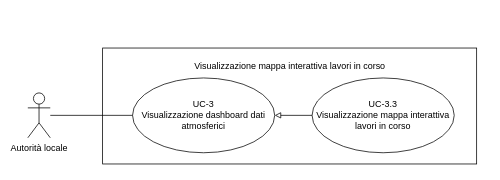
\includegraphics[width=0.5\textwidth]{analisi_dei_requisiti/UC-3.3.png}
	\captionof{figure}{UC-3.3: Visualizzazione \href{https://7last.github.io/docs/pb/documentazione-interna/glossario\#dashboard}{dashboard\textsubscript{G}} qualità dell'aria}
\end{center}

\newpage
\subsubsubsubsection{UC-3.3.1: Visualizzazione grafico time series qualità dell'aria}
\begin{itemize}
	\item \textbf{Attore principale}: autorità locale.
	\item \textbf{Precondizioni}:
	      \begin{enumerate}
		      \item l'autorità locale ha effettuato l'accesso al sistema ed esso è in funzione;
		      \item il sistema ha caricato la \href{https://7last.github.io/docs/pb/documentazione-interna/glossario\#dashboard}{dashboard\textsubscript{G}} relativa ai sensori ambientali.
	      \end{enumerate}
	\item \textbf{Postcondizioni}: l'autorità locale visualizza un grafico \href{https://7last.github.io/docs/pb/documentazione-interna/glossario\#time-series}{time series\textsubscript{G}} contenente le misurazioni storiche
	      di qualità dell'aria aggregate per 5 minuti.
	\item \textbf{Scenario principale}:
	      \begin{enumerate}
		      \item l'autorità locale accede alla piattaforma;
		      \item il sistema carica i dati relativi ai sensori interrogando il database;
		      \item l'autorità locale seleziona la visualizzazione della \href{https://7last.github.io/docs/pb/documentazione-interna/glossario\#dashboard}{dashboard\textsubscript{G}} relativa ai sensori ambientali.
	      \end{enumerate}
	\item \href{https://7last.github.io/docs/pb/documentazione-interna/glossario\#user-story}{\textbf{User story}\textsubscript{G}}:
	      come autorità locale desidero poter visualizzare un grafico \href{https://7last.github.io/docs/pb/documentazione-interna/glossario\#time-series}{time series\textsubscript{G}} contenente le misurazioni storiche
	      di qualità dell'aria per poter monitorarne l'andamento nel tempo e facilmente individuare eventuali anomalie.
\end{itemize}
\begin{center}
	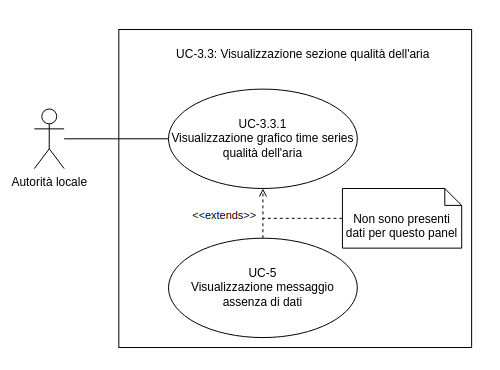
\includegraphics[width=0.5\textwidth]{analisi_dei_requisiti/UC-3.3.1.png}
	\captionof{figure}{UC-3.3.1: Visualizzazione grafico \href{https://7last.github.io/docs/pb/documentazione-interna/glossario\#time-series}{time series\textsubscript{G}} qualità dell'aria}
\end{center}

\newpage
\subsubsubsubsection{UC-3.3.2: Visualizzazione mappa interattiva sensori qualità dell'aria}
\begin{itemize}
	\item \textbf{Attore principale}: autorità locale.
	\item \textbf{Precondizioni}:
	      \begin{enumerate}
		      \item l'autorità locale ha effettuato l'accesso al sistema ed esso è in funzione;
		      \item il sistema ha caricato la \href{https://7last.github.io/docs/pb/documentazione-interna/glossario\#dashboard}{dashboard\textsubscript{G}} relativa ai sensori ambientali.
	      \end{enumerate}
	\item \textbf{Postcondizioni}: l'autorità locale visualizza una mappa interattiva popolata con dei \textit{marker} contenenti l'identificativo e le coordinate geografiche dei sensori della qualità dell'aria.
	\item \textbf{Scenario principale}:
	      \begin{enumerate}
		      \item l'autorità locale accede alla piattaforma;
		      \item il sistema carica i dati relativi ai sensori interrogando il database;
		      \item l'autorità locale seleziona la visualizzazione della \href{https://7last.github.io/docs/pb/documentazione-interna/glossario\#dashboard}{dashboard\textsubscript{G}} relativa ai sensori della qualità dell'aria.
	      \end{enumerate}
	\item \href{https://7last.github.io/docs/pb/documentazione-interna/glossario\#user-story}{\textbf{User story}\textsubscript{G}}:
	      come autorità locale desidero poter visualizzare una mappa interattiva popolata con dei \textit{marker} rappresentanti la posizione dei sensori della qualità dell'aria
	      e contenenti il loro identificativo. Essa mi consentirà di visualizzare la distribuzione dei sensori della qualità dell'aria nel territorio ed eventualmente intervenire nel caso in cui siano presenti zone non coperte.
\end{itemize}
\begin{center}
	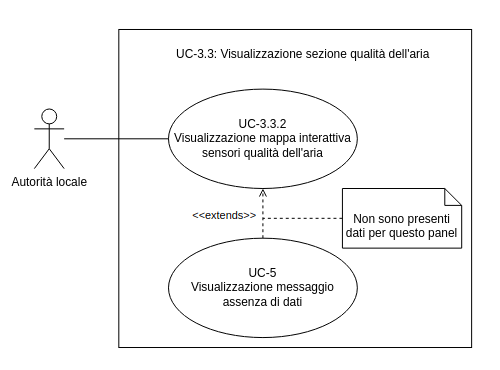
\includegraphics[width=0.5\textwidth]{analisi_dei_requisiti/UC-3.3.2.png}
	\captionof{figure}{UC-3.3.2: Visualizzazione mappa interattiva sensori qualità dell'aria}
\end{center}

\newpage
\subsubsubsubsection{UC-3.3.3: Visualizzazione \textit{panel} qualità dell'aria media nel periodo di tempo selezionato}
\begin{itemize}
	\item \textbf{Attore principale}: autorità locale.
	\item \textbf{Precondizioni}:
	      \begin{enumerate}
		      \item l'autorità locale ha effettuato l'accesso al sistema ed esso è in funzione;
		      \item il sistema ha caricato la \href{https://7last.github.io/docs/pb/documentazione-interna/glossario\#dashboard}{dashboard\textsubscript{G}} relativa ai sensori ambientali.
	      \end{enumerate}
	\item \textbf{Postcondizioni}: l'autorità locale visualizza un \href{https://7last.github.io/docs/pb/documentazione-interna/glossario\#panel}{\textit{panel}\textsubscript{G}} contenente qualità dell'aria media nel periodo di tempo selezionato.
	\item \textbf{Scenario principale}:
	      \begin{enumerate}
		      \item l'autorità locale accede alla piattaforma;
		      \item il sistema carica i dati relativi ai sensori interrogando il database;
		      \item l'autorità locale seleziona la visualizzazione della \href{https://7last.github.io/docs/pb/documentazione-interna/glossario\#dashboard}{dashboard\textsubscript{G}} relativa ai sensori ambientali.
	      \end{enumerate}
	\item \href{https://7last.github.io/docs/pb/documentazione-interna/glossario\#user-story}{\textbf{User story}\textsubscript{G}}: come autorità locale desidero poter visualizzare della qualità dell'aria media nel periodo di tempo selezionato
	      in modo da poterne monitorare l'andamento.
\end{itemize}
\begin{center}
	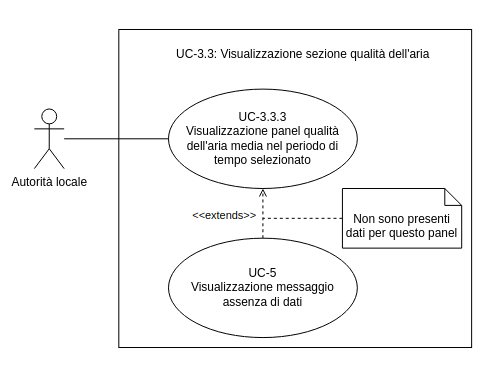
\includegraphics[width=0.5\textwidth]{analisi_dei_requisiti/UC-3.3.3.png}
	\captionof{figure}{UC-3.3.3: Visualizzazione \href{https://7last.github.io/docs/pb/documentazione-interna/glossario\#panel}{\textit{panel}\textsubscript{G}} qualità dell'aria media nel periodo di tempo selezionato}
\end{center}

\newpage
\subsubsubsubsection{UC-3.3.4: Visualizzazione \textit{panel} qualità dell'aria in tempo reale}
\begin{itemize}
	\item \textbf{Attore principale}: autorità locale.
	\item \textbf{Precondizioni}:
	      \begin{enumerate}
		      \item l'autorità locale ha effettuato l'accesso al sistema ed esso è in funzione;
		      \item il sistema ha caricato la \href{https://7last.github.io/docs/pb/documentazione-interna/glossario\#dashboard}{dashboard\textsubscript{G}} relativa ai sensori ambientali.
	      \end{enumerate}
	\item \textbf{Postcondizioni}: l'autorità locale visualizza un \href{https://7last.github.io/docs/pb/documentazione-interna/glossario\#panel}{\textit{panel}\textsubscript{G}} contenente qualità dell'aria in tempo reale.
	\item \textbf{Scenario principale}:
	      \begin{enumerate}
		      \item l'autorità locale accede alla piattaforma;
		      \item il sistema carica i dati relativi ai sensori interrogando il database;
		      \item l'autorità locale seleziona la visualizzazione della \href{https://7last.github.io/docs/pb/documentazione-interna/glossario\#dashboard}{dashboard\textsubscript{G}} relativa ai sensori ambientali.
	      \end{enumerate}
	\item \href{https://7last.github.io/docs/pb/documentazione-interna/glossario\#user-story}{\textbf{User story}\textsubscript{G}}:
	      come autorità locale desidero poter visualizzare della qualità dell'aria in tempo reale in modo da poterne monitorare l'andamento
	      e poterla facilmente confrontare con i dati storici.
\end{itemize}
\begin{center}
	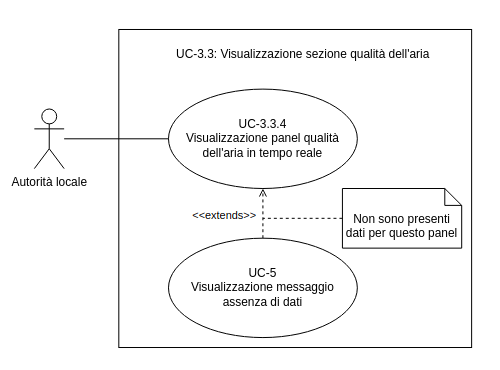
\includegraphics[width=0.5\textwidth]{analisi_dei_requisiti/UC-3.3.4.png}
	\captionof{figure}{UC-3.3.4: Visualizzazione \href{https://7last.github.io/docs/pb/documentazione-interna/glossario\#panel}{\textit{panel}\textsubscript{G}} qualità dell'aria in tempo reale}
\end{center}

\newpage
\subsubsubsubsection{UC-3.3.5: Visualizzazione \textit{panel} giorno con qualità dell'aria peggiore nel periodo di tempo selezionato}
\begin{itemize}
	\item \textbf{Attore principale}: autorità locale.
	\item \textbf{Precondizioni}:
	      \begin{enumerate}
		      \item l'autorità locale ha effettuato l'accesso al sistema ed esso è in funzione;
		      \item il sistema ha caricato la \href{https://7last.github.io/docs/pb/documentazione-interna/glossario\#dashboard}{dashboard\textsubscript{G}} relativa ai sensori ambientali.
	      \end{enumerate}
	\item \textbf{Postcondizioni}: l'autorità locale visualizza un \href{https://7last.github.io/docs/pb/documentazione-interna/glossario\#panel}{\textit{panel}\textsubscript{G}} contenente il giorno con la qualità dell'aria peggiore nel periodo di tempo selezionato.
	\item \textbf{Scenario principale}:
	      \begin{enumerate}
		      \item l'autorità locale accede alla piattaforma;
		      \item il sistema carica i dati relativi ai sensori interrogando il database;
		      \item l'autorità locale seleziona la visualizzazione della \href{https://7last.github.io/docs/pb/documentazione-interna/glossario\#dashboard}{dashboard\textsubscript{G}} relativa ai sensori ambientali.
	      \end{enumerate}
	\item \href{https://7last.github.io/docs/pb/documentazione-interna/glossario\#user-story}{\textbf{User story}\textsubscript{G}}:
	      come autorità locale desidero poter visualizzare il giorno con la qualità dell'aria peggiore nel periodo di tempo selezionato
	      in modo da poterla prendere come riferimento e confrontarla con la qualità dell'aria attuale.
\end{itemize}
\begin{center}
	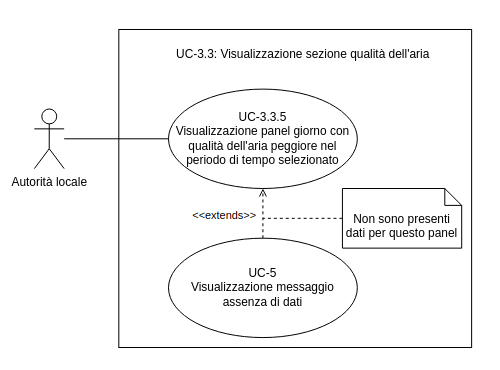
\includegraphics[width=0.5\textwidth]{analisi_dei_requisiti/UC-3.3.5.png}
	\captionof{figure}{UC-3.3.5: Visualizzazione \href{https://7last.github.io/docs/pb/documentazione-interna/glossario\#panel}{\textit{panel}\textsubscript{G}} giorno con qualità dell'aria peggiore nel periodo di tempo selezionato}
\end{center}

\newpage
\subsubsubsubsection{UC-3.3.6: Visualizzazione \textit{panel} giorno con qualità dell'aria migliore nel periodo di tempo selezionato}
\begin{itemize}
	\item \textbf{Attore principale}: autorità locale.
	\item \textbf{Precondizioni}:
	      \begin{enumerate}
		      \item l'autorità locale ha effettuato l'accesso al sistema ed esso è in funzione;
		      \item il sistema ha caricato la \href{https://7last.github.io/docs/pb/documentazione-interna/glossario\#dashboard}{dashboard\textsubscript{G}} relativa ai sensori ambientali.
	      \end{enumerate}
	\item \textbf{Postcondizioni}: l'autorità locale visualizza un \href{https://7last.github.io/docs/pb/documentazione-interna/glossario\#panel}{\textit{panel}\textsubscript{G}} contenente il giorno con la qualità dell'aria migliore nel periodo di tempo selezionato.
	\item \textbf{Scenario principale}:
	      \begin{enumerate}
		      \item l'autorità locale accede alla piattaforma;
		      \item il sistema carica i dati relativi ai sensori interrogando il database;
		      \item l'autorità locale seleziona la visualizzazione della \href{https://7last.github.io/docs/pb/documentazione-interna/glossario\#dashboard}{dashboard\textsubscript{G}} relativa ai sensori ambientali.
	      \end{enumerate}
	\item \href{https://7last.github.io/docs/pb/documentazione-interna/glossario\#user-story}{\textbf{User story}\textsubscript{G}}:
	      come autorità locale desidero poter visualizzare il giorno con la qualità dell'aria migliore nel periodo di tempo selezionato
	      in modo da poterla prendere come riferimento e confrontarla con la qualità dell'aria attuale.
\end{itemize}
\begin{center}
	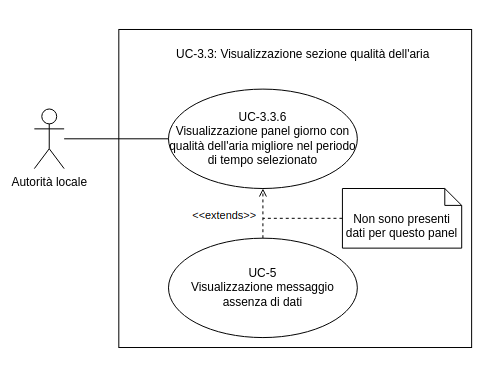
\includegraphics[width=0.5\textwidth]{analisi_dei_requisiti/UC-3.3.6.png}
	\captionof{figure}{UC-3.3.6: Visualizzazione \href{https://7last.github.io/docs/pb/documentazione-interna/glossario\#panel}{\textit{panel}\textsubscript{G}} giorno con qualità dell'aria peggiore nel periodo di tempo selezionato}
\end{center}

\newpage
\subsubsubsection{UC-3.4: Visualizzazione sezione precipitazioni}
\begin{itemize}
	\item \textbf{Attore principale}: autorità locale.
	\item \textbf{Precondizioni}: l'autorità locale ha effettuato l'accesso al sistema ed esso è in funzione.
	\item \textbf{Postcondizioni}: l'autorità locale visualizza la \href{https://7last.github.io/docs/pb/documentazione-interna/glossario\#dashboard}{dashboard\textsubscript{G}} relativa ai sensori ambientali presenti nella città, la quale contiene un grafico time series con le misurazioni storiche delle precipitazioni, una mappa dei sensori di precipitazioni collegati al sistema, dei panel che mostrano le precipitazioni medie, minime e massime nel periodo di tempo selezionato e quelle attuali.
	\item \textbf{Scenario principale}:
	      \begin{enumerate}
		      \item l'autorità locale accede alla piattaforma;
		      \item il sistema carica i dati trasmessi dai sensori interrogando il database;
		      \item l'autorità locale seleziona la visualizzazione della \href{https://7last.github.io/docs/pb/documentazione-interna/glossario\#dashboard}{dashboard\textsubscript{G}} relativa ai sensori ambientali.
	      \end{enumerate}
	\item \href{https://7last.github.io/docs/pb/documentazione-interna/glossario\#user-story}{\textbf{User story}\textsubscript{G}}:
	      come autorità locale desidero poter visualizzare una \href{https://7last.github.io/docs/pb/documentazione-interna/glossario\#dashboard}{dashboard\textsubscript{G}} relativa ai sensori ambientali presenti nella città, la quale conterrà un grafico time series con le misurazioni storiche delle precipitazioni, una mappa dei sensori di precipitazioni collegati al sistema, dei panel che mostrano le precipitazioni medie, minime e massime nel periodo di tempo selezionato e quelle attuali.
\end{itemize}
\begin{center}
	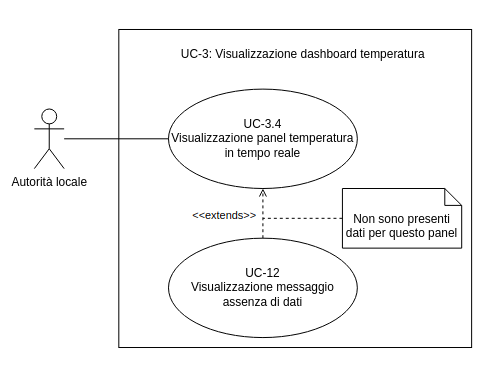
\includegraphics[width=0.5\textwidth]{analisi_dei_requisiti/UC-3.4.png}
	\captionof{figure}{UC-3.4: Visualizzazione sezione precipitazioni}
\end{center}

\newpage
\subsubsubsubsection{UC-3.4.1: Visualizzazione grafico time series quantità precipitazioni nel periodo di tempo selezionato}
\begin{itemize}
	\item \textbf{Attore principale}: autorità locale.
	\item \textbf{Precondizioni}:
	      \begin{enumerate}
		      \item l'autorità locale ha effettuato l'accesso al sistema ed esso è in funzione;
		      \item il sistema ha caricato la \href{https://7last.github.io/docs/pb/documentazione-interna/glossario\#dashboard}{dashboard\textsubscript{G}} relativa ai sensori ambientali
	      \end{enumerate}
	\item \textbf{Postcondizioni}: l'autorità locale visualizza un grafico \href{https://7last.github.io/docs/pb/documentazione-interna/glossario\#time-series}{time series\textsubscript{G}} contenente le misurazioni storiche
	      di precipitazioni aggregate per 5 minuti.
	\item \textbf{Scenario principale}:
	      \begin{enumerate}
		      \item l'autorità locale accede alla piattaforma;
		      \item il sistema carica i dati relativi ai sensori interrogando il database;
		      \item l'autorità locale seleziona la visualizzazione della \href{https://7last.github.io/docs/pb/documentazione-interna/glossario\#dashboard}{dashboard\textsubscript{G}} relativa ai sensori ambientali.
	      \end{enumerate}
	\item \href{https://7last.github.io/docs/pb/documentazione-interna/glossario\#user-story}{\textbf{User story}\textsubscript{G}}:
	      come autorità locale desidero poter visualizzare un grafico \href{https://7last.github.io/docs/pb/documentazione-interna/glossario\#time-series}{time series\textsubscript{G}} contenente le misurazioni storiche
	      di precipitazioni per poter monitorarne l'andamento nel tempo e facilmente individuare eventuali anomalie.
\end{itemize}
\begin{center}
	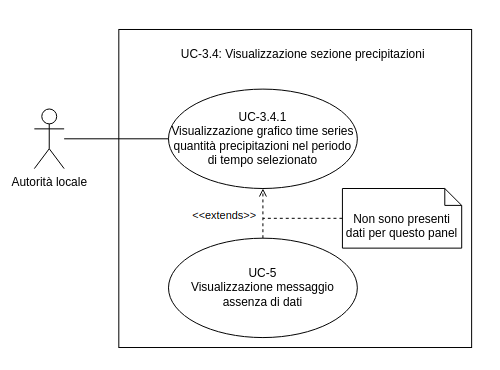
\includegraphics[width=0.5\textwidth]{analisi_dei_requisiti/UC-3.4.1.png}
	\captionof{figure}{UC-3.4.1: Visualizzazione grafico \href{https://7last.github.io/docs/pb/documentazione-interna/glossario\#time-series}{time series\textsubscript{G}} precipitazioni}
\end{center}

\newpage
\subsubsubsubsection{UC-3.4.2: Visualizzazione mappa sensori precipitazioni}
\begin{itemize}
	\item \textbf{Attore principale}: autorità locale.
	\item \textbf{Precondizioni}:
	      \begin{enumerate}
		      \item l'autorità locale ha effettuato l'accesso al sistema ed esso è in funzione;
		      \item il sistema ha caricato la \href{https://7last.github.io/docs/pb/documentazione-interna/glossario\#dashboard}{dashboard\textsubscript{G}} relativa ai sensori ambientali.
	      \end{enumerate}
	\item \textbf{Postcondizioni}: l'autorità locale visualizza una mappa interattiva popolata con dei \textit{marker} contenenti l'identificativo e le coordinate geografiche dei sensori di precipitazioni.
	\item \textbf{Scenario principale}:
	      \begin{enumerate}
		      \item l'autorità locale accede alla piattaforma;
		      \item il sistema carica i dati relativi ai sensori interrogando il database;
		      \item l'autorità locale seleziona la visualizzazione della \href{https://7last.github.io/docs/pb/documentazione-interna/glossario\#dashboard}{dashboard\textsubscript{G}} relativa ai sensori ambientali.
	      \end{enumerate}
	\item \href{https://7last.github.io/docs/pb/documentazione-interna/glossario\#user-story}{\textbf{User story}\textsubscript{G}}:
	      come autorità locale desidero poter visualizzare una mappa interattiva popolata con dei \textit{marker} rappresentanti la posizione dei sensori di precipitazioni
	      e contenenti il loro identificativo. Essa mi consentirà di visualizzare la distribuzione dei sensori di precipitazioni nel territorio ed
	      eventualmente intervenire nel caso in cui siano presenti zone non coperte.
\end{itemize}
\begin{center}
	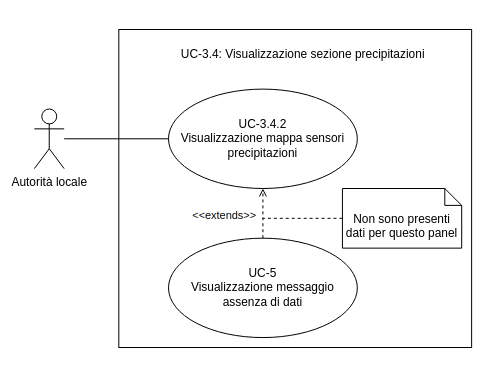
\includegraphics[width=0.5\textwidth]{analisi_dei_requisiti/UC-3.4.2.png}
	\captionof{figure}{UC-3.4.2: Visualizzazione mappa interattiva sensori precipitazioni}
\end{center}

\newpage
\subsubsubsubsection{UC-3.4.3: Visualizzazione \textit{panel} quantità di precipitazioni media nel periodo di tempo selezionato}
\begin{itemize}
	\item \textbf{Attore principale}: autorità locale.
	\item \textbf{Precondizioni}:
	      \begin{enumerate}
		      \item l'autorità locale ha effettuato l'accesso al sistema ed esso è in funzione;
		      \item il sistema ha caricato la \href{https://7last.github.io/docs/pb/documentazione-interna/glossario\#dashboard}{dashboard\textsubscript{G}} relativa ai sensori ambientali.
	      \end{enumerate}
	\item \textbf{Postcondizioni}: l'autorità locale visualizza un \href{https://7last.github.io/docs/pb/documentazione-interna/glossario\#panel}{\textit{panel}\textsubscript{G}} contenente di quantità di precipitazioni media nel periodo di tempo selezionato.
	\item \textbf{Scenario principale}:
	      \begin{enumerate}
		      \item l'autorità locale accede alla piattaforma;
		      \item il sistema carica i dati relativi ai sensori interrogando il database;
		      \item l'autorità locale seleziona la visualizzazione della \href{https://7last.github.io/docs/pb/documentazione-interna/glossario\#dashboard}{dashboard\textsubscript{G}} relativa ai sensori ambientali.
	      \end{enumerate}
	\item \href{https://7last.github.io/docs/pb/documentazione-interna/glossario\#user-story}{\textbf{User story}\textsubscript{G}}: come autorità locale desidero poter visualizzare di quantità di precipitazioni media nel periodo di tempo selezionato
	      in modo da poterne monitorare l'andamento.
\end{itemize}
\begin{center}
	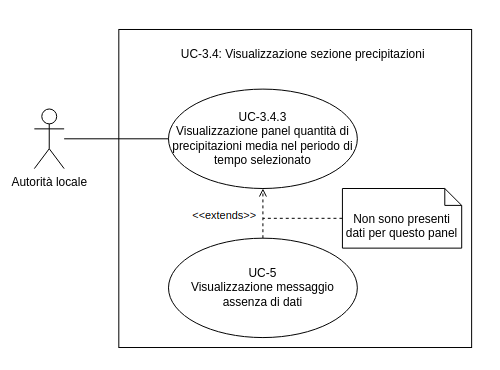
\includegraphics[width=0.5\textwidth]{analisi_dei_requisiti/UC-3.4.3.png}
	\captionof{figure}{UC-3.4.3: Visualizzazione \href{https://7last.github.io/docs/pb/documentazione-interna/glossario\#panel}{\textit{panel}\textsubscript{G}} quantità di precipitazioni media nel periodo di tempo selezionato}
\end{center}

\newpage
\subsubsubsubsection{UC-3.4.4: Visualizzazione \textit{panel} quantità di precipitazioni in tempo reale}
\begin{itemize}
	\item \textbf{Attore principale}: autorità locale.
	\item \textbf{Precondizioni}:
	      \begin{enumerate}
		      \item l'autorità locale ha effettuato l'accesso al sistema ed esso è in funzione;
		      \item il sistema ha caricato la \href{https://7last.github.io/docs/pb/documentazione-interna/glossario\#dashboard}{dashboard\textsubscript{G}} relativa ai sensori ambientali.
	      \end{enumerate}
	\item \textbf{Postcondizioni}: l'autorità locale visualizza un \href{https://7last.github.io/docs/pb/documentazione-interna/glossario\#panel}{\textit{panel}\textsubscript{G}} contenente di quantità di precipitazioni in tempo reale.
	\item \textbf{Scenario principale}:
	      \begin{enumerate}
		      \item l'autorità locale accede alla piattaforma;
		      \item il sistema carica i dati relativi ai sensori interrogando il database;
		      \item l'autorità locale seleziona la visualizzazione della \href{https://7last.github.io/docs/pb/documentazione-interna/glossario\#dashboard}{dashboard\textsubscript{G}} relativa ai sensori ambientali.
	      \end{enumerate}
	\item \href{https://7last.github.io/docs/pb/documentazione-interna/glossario\#user-story}{\textbf{User story}\textsubscript{G}}:
	      come autorità locale desidero poter visualizzare di quantità di precipitazioni in tempo reale in modo da poterne monitorare l'andamento
	      e poterla facilmente confrontare con i dati storici.
\end{itemize}
\begin{center}
	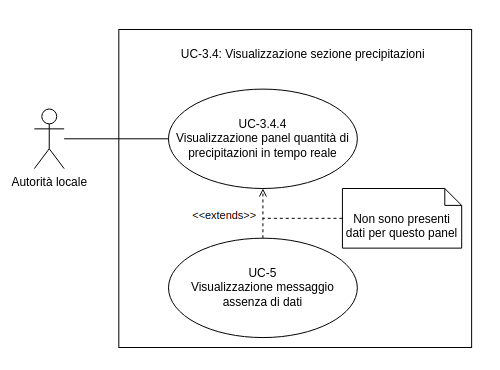
\includegraphics[width=0.5\textwidth]{analisi_dei_requisiti/UC-3.4.4.png}
	\captionof{figure}{UC-3.4.4: Visualizzazione \href{https://7last.github.io/docs/pb/documentazione-interna/glossario\#panel}{\textit{panel}\textsubscript{G}} quantità di precipitazioni in tempo reale}
\end{center}

\newpage
\subsubsubsubsection{UC-3.4.5: Visualizzazione \textit{panel} giorno con precipitazioni maggiori nel periodo di tempo selezionato}
\begin{itemize}
	\item \textbf{Attore principale}: autorità locale.
	\item \textbf{Precondizioni}:
	      \begin{enumerate}
		      \item l'autorità locale ha effettuato l'accesso al sistema ed esso è in funzione;
		      \item il sistema ha caricato la \href{https://7last.github.io/docs/pb/documentazione-interna/glossario\#dashboard}{dashboard\textsubscript{G}} relativa ai sensori ambientali.
	      \end{enumerate}
	\item \textbf{Postcondizioni}: l'autorità locale visualizza un \href{https://7last.github.io/docs/pb/documentazione-interna/glossario\#panel}{\textit{panel}\textsubscript{G}} contenente il giorno con la quantità di precipitazioni maggiori nel periodo di tempo selezionato.
	\item \textbf{Scenario principale}:
	      \begin{enumerate}
		      \item l'autorità locale accede alla piattaforma;
		      \item il sistema carica i dati relativi ai sensori interrogando il database;
		      \item l'autorità locale seleziona la visualizzazione della \href{https://7last.github.io/docs/pb/documentazione-interna/glossario\#dashboard}{dashboard\textsubscript{G}} relativa ai sensori ambientali.
	      \end{enumerate}
	\item \href{https://7last.github.io/docs/pb/documentazione-interna/glossario\#user-story}{\textbf{User story}\textsubscript{G}}:
	      come autorità locale desidero poter visualizzare il giorno con la quantità di precipitazioni maggiori nel periodo di tempo selezionato
	      e poterla facilmente confrontare con i dati storici.
\end{itemize}
\begin{center}
	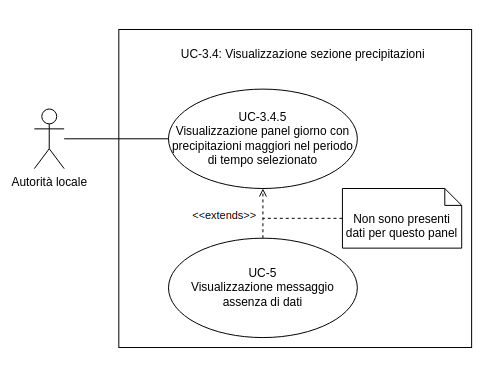
\includegraphics[width=0.5\textwidth]{analisi_dei_requisiti/UC-3.4.5.png}
	\captionof{figure}{UC-3.4.5: Visualizzazione \href{https://7last.github.io/docs/pb/documentazione-interna/glossario\#panel}{\textit{panel}\textsubscript{G}} giorno con precipitazioni maggiori nel periodo di tempo selezionato}
\end{center}

\newpage
\subsubsubsubsection{UC-3.4.6: Visualizzazione \textit{panel} giorno con precipitazioni minori nel periodo di tempo selezionato}
\begin{itemize}
	\item \textbf{Attore principale}: autorità locale.
	\item \textbf{Precondizioni}:
	      \begin{enumerate}
		      \item l'autorità locale ha effettuato l'accesso al sistema ed esso è in funzione;
		      \item il sistema ha caricato la \href{https://7last.github.io/docs/pb/documentazione-interna/glossario\#dashboard}{dashboard\textsubscript{G}} relativa ai sensori ambientali.
	      \end{enumerate}
	\item \textbf{Postcondizioni}: l'autorità locale visualizza un \href{https://7last.github.io/docs/pb/documentazione-interna/glossario\#panel}{\textit{panel}\textsubscript{G}} contenente il giorno con la quantità di precipitazioni minori nel periodo di tempo selezionato.
	\item \textbf{Scenario principale}:
	      \begin{enumerate}
		      \item l'autorità locale accede alla piattaforma;
		      \item il sistema carica i dati relativi ai sensori interrogando il database;
		      \item l'autorità locale seleziona la visualizzazione della \href{https://7last.github.io/docs/pb/documentazione-interna/glossario\#dashboard}{dashboard\textsubscript{G}} relativa ai sensori ambientali.
	      \end{enumerate}
	\item \href{https://7last.github.io/docs/pb/documentazione-interna/glossario\#user-story}{\textbf{User story}\textsubscript{G}}:
	      come autorità locale desidero poter visualizzare il giorno con la quantità di precipitazioni minori nel periodo di tempo selezionato
	      e poterla facilmente confrontare con i dati storici.
\end{itemize}
\begin{center}
	\includegraphics[width=0.5\textwidth]{analisi_dei_requisiti/UC-3.4.6.png}
	\captionof{figure}{UC-3.4.6: Visualizzazione \href{https://7last.github.io/docs/pb/documentazione-interna/glossario\#panel}{\textit{panel}\textsubscript{G}} giorno con precipitazioni minori nel periodo di tempo selezionato}
\end{center}

\newpage
\subsubsubsection{UC-3.5: Visualizzazione sezione livello dei fiumi}
\begin{itemize}
	\item \textbf{Attore principale}: autorità locale.
	\item \textbf{Precondizioni}: l'autorità locale ha effettuato l'accesso al sistema ed esso è in funzione.
	\item \textbf{Postcondizioni}: l'autorità locale visualizza la \href{https://7last.github.io/docs/pb/documentazione-interna/glossario\#dashboard}{dashboard\textsubscript{G}} relativa ai sensori ambientali presenti nella città, la quale contiene un grafico time series con le misurazioni storiche del livello dei fiumi, una mappa dei sensori di livello dei fiumi collegati al sistema, dei panel che mostrano il livello dei fiumi medio, minimo e massimo nel periodo di tempo selezionato e quello attuale.
	\item \textbf{Scenario principale}:
	      \begin{enumerate}
		      \item l'autorità locale accede alla piattaforma;
		      \item il sistema carica i dati trasmessi dai sensori interrogando il database;
		      \item l'autorità locale seleziona la visualizzazione della \href{https://7last.github.io/docs/pb/documentazione-interna/glossario\#dashboard}{dashboard\textsubscript{G}} relativa ai sensori ambientali.
	      \end{enumerate}
	\item \href{https://7last.github.io/docs/pb/documentazione-interna/glossario\#user-story}{\textbf{User story}\textsubscript{G}}:
	      come autorità locale desidero poter visualizzare una \href{https://7last.github.io/docs/pb/documentazione-interna/glossario\#dashboard}{dashboard\textsubscript{G}} relativa ai sensori ambientali presenti nella città, la quale conterrà un grafico time series con le misurazioni storiche del livello dei fiumi, una mappa dei sensori di livello dei fiumi collegati al sistema, dei panel che mostrano il livello dei fiumi medio, minimo e massimo nel periodo di tempo selezionato e quello attuale.
\end{itemize}
\begin{center}
	\includegraphics[width=0.5\textwidth]{analisi_dei_requisiti/UC-3.5.png}
	\captionof{figure}{UC-3.5: Visualizzazione sezione livello dei fiumi}
\end{center}

\newpage
\subsubsubsubsection{UC-3.5.1: Visualizzazione grafico time series livello dei fiumi}
\begin{itemize}
	\item \textbf{Attore principale}: autorità locale.
	\item \textbf{Precondizioni}:
	      \begin{enumerate}
		      \item l'autorità locale ha effettuato l'accesso al sistema ed esso è in funzione;
		      \item il sistema ha caricato la \href{https://7last.github.io/docs/pb/documentazione-interna/glossario\#dashboard}{dashboard\textsubscript{G}} relativa ai sensori ambientali.
	      \end{enumerate}
	\item \textbf{Postcondizioni}: l'autorità locale visualizza un grafico \href{https://7last.github.io/docs/pb/documentazione-interna/glossario\#time-series}{time series\textsubscript{G}} contenente le misurazioni storiche
	      del livello dei fiumi aggregate per 5 minuti.
	\item \textbf{Scenario principale}:
	      \begin{enumerate}
		      \item l'autorità locale accede alla piattaforma;
		      \item il sistema carica i dati relativi ai sensori interrogando il database;
		      \item l'autorità locale seleziona la visualizzazione della \href{https://7last.github.io/docs/pb/documentazione-interna/glossario\#dashboard}{dashboard\textsubscript{G}} relativa ai sensori ambientali.
	      \end{enumerate}
	\item \href{https://7last.github.io/docs/pb/documentazione-interna/glossario\#user-story}{\textbf{User story}\textsubscript{G}}:
	      come autorità locale desidero poter visualizzare un grafico \href{https://7last.github.io/docs/pb/documentazione-interna/glossario\#time-series}{time series\textsubscript{G}} contenente le misurazioni storiche
	      del livello dei fiumi per poter monitorarne l'andamento nel tempo e facilmente individuare eventuali anomalie.
\end{itemize}
\begin{center}
	\includegraphics[width=0.5\textwidth]{analisi_dei_requisiti/UC-3.5.1.png}
	\captionof{figure}{UC-3.5.1, Visualizzazione grafico \href{https://7last.github.io/docs/pb/documentazione-interna/glossario\#time-series}{time series\textsubscript{G}} livello dei fiumi}
\end{center}

\newpage
\subsubsubsubsection{UC-3.5.2: Visualizzazione mappa sensori livello dei fiumi}
\begin{itemize}
	\item \textbf{Attore principale}: autorità locale.
	\item \textbf{Precondizioni}:
	      \begin{enumerate}
		      \item l'autorità locale ha effettuato l'accesso al sistema ed esso è in funzione;
		      \item il sistema ha caricato la \href{https://7last.github.io/docs/pb/documentazione-interna/glossario\#dashboard}{dashboard\textsubscript{G}} relativa ai sensori ambientali.
	      \end{enumerate}
	\item \textbf{Postcondizioni}: l'autorità locale visualizza una mappa interattiva popolata con dei \textit{marker} contenenti l'identificativo e le coordinate geografiche dei sensori del livello dei fiumi.
	\item \textbf{Scenario principale}:
	      \begin{enumerate}
		      \item l'autorità locale accede alla piattaforma;
		      \item il sistema carica i dati relativi ai sensori interrogando il database;
		      \item l'autorità locale seleziona la visualizzazione della \href{https://7last.github.io/docs/pb/documentazione-interna/glossario\#dashboard}{dashboard\textsubscript{G}} relativa ai sensori ambientali.
	      \end{enumerate}
	\item \href{https://7last.github.io/docs/pb/documentazione-interna/glossario\#user-story}{\textbf{User story}\textsubscript{G}}:
	      come autorità locale desidero poter visualizzare una mappa interattiva popolata con dei \textit{marker} rappresentanti la posizione dei sensori del livello dei fiumi
	      e contenenti il loro identificativo. Essa mi consentirà di visualizzare la distribuzione dei sensori del livello dei fiumi nel territorio ed eventualmente intervenire nel caso in cui siano presenti zone non coperte.
\end{itemize}
\begin{center}
	\includegraphics[width=0.5\textwidth]{analisi_dei_requisiti/UC-3.5.2.png}
	\captionof{figure}{UC-3.5.2: Visualizzazione mappa interattiva sensori livello dei fiumi}
\end{center}

\newpage
\subsubsubsubsection{UC-3.5.3: Visualizzazione \textit{panel} livello dei fiumi medio nel periodo di tempo selezionato}
\begin{itemize}
	\item \textbf{Attore principale}: autorità locale.
	\item \textbf{Precondizioni}:
	      \begin{enumerate}
		      \item l'autorità locale ha effettuato l'accesso al sistema ed esso è in funzione;
		      \item il sistema ha caricato la \href{https://7last.github.io/docs/pb/documentazione-interna/glossario\#dashboard}{dashboard\textsubscript{G}} relativa ai sensori ambientali.
	      \end{enumerate}
	\item \textbf{Postcondizioni}: l'autorità locale visualizza un \href{https://7last.github.io/docs/pb/documentazione-interna/glossario\#panel}{\textit{panel}\textsubscript{G}} contenente del livello dei fiumi medio nel periodo di tempo selezionato.
	\item \textbf{Scenario principale}:
	      \begin{enumerate}
		      \item l'autorità locale accede alla piattaforma;
		      \item il sistema carica i dati relativi ai sensori interrogando il database;
		      \item l'autorità locale seleziona la visualizzazione della \href{https://7last.github.io/docs/pb/documentazione-interna/glossario\#dashboard}{dashboard\textsubscript{G}} relativa ai sensori ambientali.
	      \end{enumerate}
	\item \href{https://7last.github.io/docs/pb/documentazione-interna/glossario\#user-story}{\textbf{User story}\textsubscript{G}}:
	      come autorità locale desidero poter visualizzare del livello dei fiumi medio nel periodo di tempo selezionato
	      in modo da poterne monitorare l'andamento.
\end{itemize}
\begin{center}
	\includegraphics[width=0.5\textwidth]{analisi_dei_requisiti/UC-3.5.3.png}
	\captionof{figure}{UC-3.5.3: Visualizzazione \href{https://7last.github.io/docs/pb/documentazione-interna/glossario\#panel}{\textit{panel}\textsubscript{G}} livello dei fiumi medio nel periodo di tempo selezionato}
\end{center}

\newpage
\subsubsubsubsection{UC-3.5.4: Visualizzazione \textit{panel} livello dei fiumi in tempo reale}
\begin{itemize}
	\item \textbf{Attore principale}: autorità locale.
	\item \textbf{Precondizioni}:
	      \begin{enumerate}
		      \item l'autorità locale ha effettuato l'accesso al sistema ed esso è in funzione;
		      \item il sistema ha caricato la \href{https://7last.github.io/docs/pb/documentazione-interna/glossario\#dashboard}{dashboard\textsubscript{G}} relativa ai sensori ambientali.
	      \end{enumerate}
	\item \textbf{Postcondizioni}: l'autorità locale visualizza un \href{https://7last.github.io/docs/pb/documentazione-interna/glossario\#panel}{\textit{panel}\textsubscript{G}} contenente il livello dei fiumi in tempo reale.
	\item \textbf{Scenario principale}:
	      \begin{enumerate}
		      \item l'autorità locale accede alla piattaforma;
		      \item il sistema carica i dati relativi ai sensori interrogando il database;
		      \item l'autorità locale seleziona la visualizzazione della \href{https://7last.github.io/docs/pb/documentazione-interna/glossario\#dashboard}{dashboard\textsubscript{G}} relativa ai sensori ambientali.
	      \end{enumerate}
	\item \href{https://7last.github.io/docs/pb/documentazione-interna/glossario\#user-story}{\textbf{User story}\textsubscript{G}}:
	      come autorità locale desidero poter visualizzare il livello dei fiumi in tempo reale in modo da poterne monitorare l'andamento
	      e poterlo facilmente confrontare con i dati storici.
\end{itemize}
\begin{center}
	\includegraphics[width=0.5\textwidth]{analisi_dei_requisiti/UC-3.5.4.png}
	\captionof{figure}{UC-3.5.4: Visualizzazione \href{https://7last.github.io/docs/pb/documentazione-interna/glossario\#panel}{\textit{panel}\textsubscript{G}} livello dei fiumi in tempo reale}
\end{center}


%%%%%%%%%%%%%%%%%%%%%%%%%%%%%%%%%%%%%%%%%%%%%%%%%%%%%%%INIZIO URBANI%%%%%%%%%%%%%%%%%%%%%%%%%%%%%%%%%%%%%%%%%%%

\newpage
\subsubsection{UC-4: Visualizzazione dashboard dati urbani}
\begin{itemize}
	\item \textbf{Attore principale}: autorità locale.
	\item \textbf{Precondizioni}: l'autorità locale ha effettuato l'accesso al sistema ed esso è in funzione.
	\item \textbf{Postcondizioni}: l'autorità locale visualizza la \href{https://7last.github.io/docs/pb/documentazione-interna/glossario\#dashboard}{dashboard\textsubscript{G}} contenente le sezioni relative ai sensori urbani presenti nella città.
	\item \textbf{Scenario principale}:
	      \begin{enumerate}
		      \item l'autorità locale accede alla piattaforma;
		      \item il sistema carica i dati relativi ai sensori interrogando il database.
	      \end{enumerate}
	\item \href{https://7last.github.io/docs/pb/documentazione-interna/glossario\#user-story}{\textbf{User story}\textsubscript{G}}: come autorità locale desidero poter visualizzare una \href{https://7last.github.io/docs/pb/documentazione-interna/glossario\#dashboard}{dashboard\textsubscript{G}} dei dati ambientali contenente le sezioni relative ai sensori urbani presenti nella città, la quale mi consente di monitorare la situazione urbanistica.
\end{itemize}
\begin{center}
	\includegraphics[width=0.5\textwidth]{analisi_dei_requisiti/UC-4.png}
	\captionof{figure}{UC-4: Visualizzazione \href{https://7last.github.io/docs/pb/documentazione-interna/glossario\#dashboard}{dashboard\textsubscript{G}} dei dati urbani}
\end{center}

\newpage
\subsubsubsection{UC-4.1: Visualizzazione sezione traffico}
\begin{itemize}
	\item \textbf{Attore principale}: autorità locale.
	\item \textbf{Precondizioni}: l'autorità locale ha effettuato l'accesso al sistema ed esso è in funzione.
	\item \textbf{Postcondizioni}: l'autorità locale visualizza la \href{https://7last.github.io/docs/pb/documentazione-interna/glossario\#dashboard}{dashboard\textsubscript{G}} relativa ai sensori urbani presenti nella città, la quale contiene un grafico time series con le misurazioni storiche del traffico, una mappa dei sensori di traffico collegati al sistema, un panel che mostra il numero dei veicoli in tempo reale, un panel che mostra la velocità media in tempo reale.
	\item \textbf{Scenario principale}:
	      \begin{enumerate}
		      \item l'autorità locale accede alla piattaforma;
		      \item il sistema carica i dati trasmessi dai sensori interrogando il database;
		      \item l'autorità locale seleziona la visualizzazione della \href{https://7last.github.io/docs/pb/documentazione-interna/glossario\#dashboard}{dashboard\textsubscript{G}} relativa ai sensori urbani.
	      \end{enumerate}
	\item \href{https://7last.github.io/docs/pb/documentazione-interna/glossario\#user-story}{\textbf{User story}\textsubscript{G}}:
	      come autorità locale desidero poter visualizzare una \href{https://7last.github.io/docs/pb/documentazione-interna/glossario\#dashboard}{dashboard\textsubscript{G}} relativa ai sensori urbani presenti nella città, la quale conterrà un grafico time series con le misurazioni storiche del traffico, una mappa dei sensori di traffico collegati al sistema, un panel che mostra il numero dei veicoli in tempo reale, un panel che mostra la velocità media in tempo reale.
\end{itemize}
\begin{center}
	\includegraphics[width=0.5\textwidth]{analisi_dei_requisiti/UC-4.1.png}
	\captionof{figure}{UC-4.1: Visualizzazione sezione traffico}
\end{center}

\newpage
\subsubsubsubsection{UC-4.1.1: Visualizzazione grafico time series traffico}
\begin{itemize}
	\item \textbf{Attore principale}: autorità locale.
	\item \textbf{Precondizioni}:
	      \begin{enumerate}
		      \item l'autorità locale ha effettuato l'accesso al sistema ed esso è in funzione;
		      \item il sistema ha caricato la \href{https://7last.github.io/docs/pb/documentazione-interna/glossario\#dashboard}{dashboard\textsubscript{G}} relativa ai sensori urbani.
	      \end{enumerate}
	\item \textbf{Postcondizioni}: l'autorità locale visualizza un grafico \href{https://7last.github.io/docs/pb/documentazione-interna/glossario\#time-series}{time series\textsubscript{G}} contenente le misurazioni storiche di traffico aggregate per 5 minuti.
	\item \textbf{Scenario principale}:
	      \begin{enumerate}
		      \item l'autorità locale accede alla piattaforma;
		      \item il sistema carica i dati relativi ai sensori interrogando il database;
		      \item l'autorità locale seleziona la visualizzazione della \href{https://7last.github.io/docs/pb/documentazione-interna/glossario\#dashboard}{dashboard\textsubscript{G}} relativa ai sensori urbani.
	      \end{enumerate}
	\item \href{https://7last.github.io/docs/pb/documentazione-interna/glossario\#user-story}{\textbf{User story}\textsubscript{G}}:
	      come autorità locale desidero poter visualizzare un grafico \href{https://7last.github.io/docs/pb/documentazione-interna/glossario\#time-series}{time series\textsubscript{G}} contenente le misurazioni storiche
	      di traffico per poter monitorarne l'andamento nel tempo e facilmente individuare eventuali anomalie
	      o congestioni.
\end{itemize}
\begin{center}
	\includegraphics[width=0.5\textwidth]{analisi_dei_requisiti/UC-4.1.1.png}
	\captionof{figure}{UC-4.1.1: Visualizzazione grafico \href{https://7last.github.io/docs/pb/documentazione-interna/glossario\#time-series}{time series\textsubscript{G}} traffico}
\end{center}

\newpage
\subsubsubsubsection{UC-4.1.2: Visualizzazione mappa sensori traffico}
\begin{itemize}
	\item \textbf{Attore principale}: autorità locale.
	\item \textbf{Precondizioni}:
	      \begin{enumerate}
		      \item l'autorità locale ha effettuato l'accesso al sistema ed esso è in funzione;
		      \item il sistema ha caricato la \href{https://7last.github.io/docs/pb/documentazione-interna/glossario\#dashboard}{dashboard\textsubscript{G}} relativa ai sensori urbani.
	      \end{enumerate}
	\item \textbf{Postcondizioni}: l'autorità locale visualizza una mappa interattiva popolata con dei \textit{marker} contenenti l'identificativo e le coordinate geografiche dei sensori del traffico.
	\item \textbf{Scenario principale}:
	      \begin{enumerate}
		      \item l'autorità locale accede alla piattaforma;
		      \item il sistema carica i dati relativi ai sensori interrogando il database;
		      \item l'autorità locale seleziona la visualizzazione della \href{https://7last.github.io/docs/pb/documentazione-interna/glossario\#dashboard}{dashboard\textsubscript{G}} relativa ai sensori urbani.
	      \end{enumerate}
	\item \href{https://7last.github.io/docs/pb/documentazione-interna/glossario\#user-story}{\textbf{User story}\textsubscript{G}}:
	      come autorità locale desidero poter visualizzare una mappa interattiva popolata con dei \textit{marker} rappresentanti la posizione dei sensori del traffico
	      e contenenti il loro identificativo. Essa mi consentirà di visualizzare la distribuzione dei sensori del traffico nel territorio ed eventualmente intervenire nel caso in cui siano presenti zone non coperte.
\end{itemize}
\begin{center}
	\includegraphics[width=0.5\textwidth]{analisi_dei_requisiti/UC-4.1.2.png}
	\captionof{figure}{UC-4.1.2: Visualizzazione mappa interattiva sensori traffico}
\end{center}

\newpage
\subsubsubsubsection{UC-4.1.3: Visualizzazione \textit{panel} numero veicoli in tempo reale}
\begin{itemize}
	\item \textbf{Attore principale}: autorità locale.
	\item \textbf{Precondizioni}:
	      \begin{enumerate}
		      \item l'autorità locale ha effettuato l'accesso al sistema ed esso è in funzione;
		      \item il sistema ha caricato la \href{https://7last.github.io/docs/pb/documentazione-interna/glossario\#dashboard}{dashboard\textsubscript{G}} relativa ai sensori urbani.
	      \end{enumerate}
	\item \textbf{Postcondizioni}: l'autorità locale visualizza un \href{https://7last.github.io/docs/pb/documentazione-interna/glossario\#panel}{\textit{panel}\textsubscript{G}} contenente il numero di veicoli in tempo reale.
	\item \textbf{Scenario principale}:
	      \begin{enumerate}
		      \item l'autorità locale accede alla piattaforma;
		      \item il sistema carica i dati relativi ai sensori interrogando il database;
		      \item l'autorità locale seleziona la visualizzazione della \href{https://7last.github.io/docs/pb/documentazione-interna/glossario\#dashboard}{dashboard\textsubscript{G}} relativa ai sensori urbani.
	      \end{enumerate}
	\item \href{https://7last.github.io/docs/pb/documentazione-interna/glossario\#user-story}{\textbf{User story}\textsubscript{G}}:
	      come autorità locale desidero poter visualizzare del numero di veicoli in tempo reale in modo da poterne monitorare l'andamento
	      e poterla facilmente confrontare con i dati storici.
\end{itemize}
\begin{center}
	\includegraphics[width=0.5\textwidth]{analisi_dei_requisiti/UC-4.1.3.png}
	\captionof{figure}{UC-4.1.3: Visualizzazione \href{https://7last.github.io/docs/pb/documentazione-interna/glossario\#panel}{\textit{panel}\textsubscript{G}} numero di veicoli in tempo reale}
\end{center}

\newpage
\subsubsubsubsection{UC-4.1.4: Visualizzazione \textit{panel} velocità media in tempo reale}
\begin{itemize}
	\item \textbf{Attore principale}: autorità locale.
	\item \textbf{Precondizioni}:
	      \begin{enumerate}
		      \item l'autorità locale ha effettuato l'accesso al sistema ed esso è in funzione;
		      \item il sistema ha caricato la \href{https://7last.github.io/docs/pb/documentazione-interna/glossario\#dashboard}{dashboard\textsubscript{G}} relativa ai sensori urbani.
	      \end{enumerate}
	\item \textbf{Postcondizioni}: l'autorità locale visualizza un \href{https://7last.github.io/docs/pb/documentazione-interna/glossario\#panel}{\textit{panel}\textsubscript{G}} contenente la velocità media in tempo reale.
	\item \textbf{Scenario principale}:
	      \begin{enumerate}
		      \item l'autorità locale accede alla piattaforma;
		      \item il sistema carica i dati relativi ai sensori interrogando il database;
		      \item l'autorità locale seleziona la visualizzazione della \href{https://7last.github.io/docs/pb/documentazione-interna/glossario\#dashboard}{dashboard\textsubscript{G}} relativa ai sensori urbani.
	      \end{enumerate}
	\item \href{https://7last.github.io/docs/pb/documentazione-interna/glossario\#user-story}{\textbf{User story}\textsubscript{G}}:
	      come autorità locale desidero poter visualizzare della velocità media in tempo reale in modo da poterne monitorare l'andamento
	      e poterla facilmente confrontare con i dati storici.
\end{itemize}
\begin{center}
	\includegraphics[width=0.5\textwidth]{analisi_dei_requisiti/UC-4.1.4.png}
	\captionof{figure}{UC-4.1.4: Visualizzazione \href{https://7last.github.io/docs/pb/documentazione-interna/glossario\#panel}{\textit{panel}\textsubscript{G}} velocità media in tempo reale}
\end{center}

\newpage
\subsubsubsection{UC-4.2: Visualizzazione sezione colonnine di ricarica}
\begin{itemize}
	\item \textbf{Attore principale}: autorità locale.
	\item \textbf{Precondizioni}: l'autorità locale ha effettuato l'accesso al sistema ed esso è in funzione.
	\item \textbf{Postcondizioni}: l'autorità locale visualizza la \href{https://7last.github.io/docs/pb/documentazione-interna/glossario\#dashboard}{dashboard\textsubscript{G}} relativa ai sensori urbani presenti nella città, la quale contiene una mappa dei sensori di colonnine di ricarica collegati al sistema, un grafico a barre rappresentante il tempo di utilizzo di ciascuna colonnina nel tempo selezionato, un grafico a torta con la percentuale di colonnine occupate in tempo reale, un grafico time series con i valori storici della \textit{charging efficiency}, due gauge con la percentuale di efficienza e utilizzo media nel periodo di tempo selezionato e un panel che mostra le colonnine più e meno efficienti e più e meno utilizzate.
	\item \textbf{Scenario principale}:
	      \begin{enumerate}
		      \item l'autorità locale accede alla piattaforma;
		      \item il sistema carica i dati trasmessi dai sensori interrogando il database;
		      \item l'autorità locale seleziona la visualizzazione della \href{https://7last.github.io/docs/pb/documentazione-interna/glossario\#dashboard}{dashboard\textsubscript{G}} relativa ai sensori urbani.
	      \end{enumerate}
	\item \href{https://7last.github.io/docs/pb/documentazione-interna/glossario\#user-story}{\textbf{User story}\textsubscript{G}}:
	      come autorità locale desidero poter visualizzare una \href{https://7last.github.io/docs/pb/documentazione-interna/glossario\#dashboard}{dashboard\textsubscript{G}} relativa ai sensori urbani presenti nella città, la quale conterrà una mappa dei sensori di colonnine di ricarica, un grafico a barre col tempo di utilizzo nel tempo selezionato, un grafico a torta con la percentuale di colonnine occupate in tempo reale, un grafico time series con i valori storici dell'efficienza delle colonnine, due gauge con la percentuale di efficienza e utilizzo media nel periodo di tempo selezionato e un panel che mostra le colonnine più e meno efficienti e più e meno utilizzate.
\end{itemize}
\begin{center}
	\includegraphics[width=0.5\textwidth]{analisi_dei_requisiti/UC-4.2.png}
	\captionof{figure}{UC-4.2: Visualizzazione sezione colonnine di ricarica}
\end{center}

\newpage
\subsubsubsubsection{UC-4.2.1: Visualizzazione mappa colonnine di ricarica con stato}
\begin{itemize}
	\item \textbf{Attore principale}: autorità locale.
	\item \textbf{Precondizioni}:
	      \begin{enumerate}
		      \item l'autorità locale ha effettuato l'accesso al sistema ed esso è in funzione;
		      \item il sistema ha caricato la \href{https://7last.github.io/docs/pb/documentazione-interna/glossario\#dashboard}{dashboard\textsubscript{G}} relativa ai sensori urbani.
	      \end{enumerate}
	\item \textbf{Postcondizioni}: l'autorità locale visualizza una mappa interattiva popolata con dei \textit{marker} rappresentanti la posizione delle colonnine di ricarica.
	\item \textbf{Scenario principale}:
	      \begin{enumerate}
		      \item l'autorità locale accede alla piattaforma;
		      \item il sistema carica i dati relativi ai sensori interrogando il database;
		      \item l'autorità locale seleziona la visualizzazione della \href{https://7last.github.io/docs/pb/documentazione-interna/glossario\#dashboard}{dashboard\textsubscript{G}} relativa ai sensori urbani.
	      \end{enumerate}
	\item \href{https://7last.github.io/docs/pb/documentazione-interna/glossario\#user-story}{\textbf{User story}\textsubscript{G}}:
	      come autorità locale desidero poter visualizzare una mappa interattiva popolata con dei \textit{marker} rappresentanti la posizione delle colonnine di ricarica
	      contenenti il loro identificativo e lo stato di funzionamento. Essa mi consentirà di visualizzare la distribuzione delle colonnine di ricarica nel territorio
	      ed eventualmente intervenire nel caso in cui vi siano dei guasti.
\end{itemize}
\begin{center}
	\includegraphics[width=0.5\textwidth]{analisi_dei_requisiti/UC-4.2.1.png}
	\captionof{figure}{UC-4.2.1: Visualizzazione mappa interattiva sensori colonnine di ricarica}
\end{center}

\newpage
\subsubsubsubsection{UC-4.2.2: Visualizzazione grafico a barre tempo di utilizzo colonnine di ricarica}
\begin{itemize}
	\item \textbf{Attore principale}: autorità locale.
	\item \textbf{Precondizioni}:
	      \begin{enumerate}
		      \item l'autorità locale ha effettuato l'accesso al sistema ed esso è in funzione;
		      \item il sistema ha caricato la \href{https://7last.github.io/docs/pb/documentazione-interna/glossario\#dashboard}{dashboard\textsubscript{G}} relativa ai sensori urbani.
	      \end{enumerate}
	\item \textbf{Postcondizioni}: l'autorità locale visualizza un grafico a barre contenente il tempo totale di utilizzo di ciascuna colonnina di ricarica nel tempo selezionato.
	\item \textbf{Scenario principale}:
	      \begin{enumerate}
		      \item l'autorità locale accede alla piattaforma;
		      \item il sistema carica i dati relativi ai sensori interrogando il database;
		      \item l'autorità locale seleziona la visualizzazione della \href{https://7last.github.io/docs/pb/documentazione-interna/glossario\#dashboard}{dashboard\textsubscript{G}} relativa ai sensori urbani.
	      \end{enumerate}
	\item \href{https://7last.github.io/docs/pb/documentazione-interna/glossario\#user-story}{\textbf{User story}\textsubscript{G}}:
	      come autorità locale desidero poter visualizzare un \href{https://7last.github.io/docs/pb/documentazione-interna/glossario\#panel}{\textit{panel}\textsubscript{G}} contenente il tempo totale di utilizzo di ciascuna colonnina di ricarica nel tempo selezionato
\end{itemize}
\begin{center}
	\includegraphics[width=0.5\textwidth]{analisi_dei_requisiti/UC-4.2.2.png}
	\captionof{figure}{UC-4.2.2: Visualizzazione grafico a barre tempo di utilizzo colonnine di ricarica}
\end{center}

\newpage
\subsubsubsubsection{UC-4.2.3: Visualizzazione grafico a torta percentuale di colonnine di ricarica utilizzate in tempo reale}
\begin{itemize}
	\item \textbf{Attore principale}: autorità locale.
	\item \textbf{Precondizioni}:
	      \begin{enumerate}
		      \item l'autorità locale ha effettuato l'accesso al sistema ed esso è in funzione;
		      \item il sistema ha caricato la \href{https://7last.github.io/docs/pb/documentazione-interna/glossario\#dashboard}{dashboard\textsubscript{G}} relativa ai sensori urbani.
	      \end{enumerate}
	\item \textbf{Postcondizioni}: l'autorità locale visualizza un grafico a torta contenente la percentuale di colonnine di ricarica utilizzate in tempo reale.
	\item \textbf{Scenario principale}:
	      \begin{enumerate}
		      \item l'autorità locale accede alla piattaforma;
		      \item il sistema carica i dati relativi ai sensori interrogando il database;
		      \item l'autorità locale seleziona la visualizzazione della \href{https://7last.github.io/docs/pb/documentazione-interna/glossario\#dashboard}{dashboard\textsubscript{G}} relativa ai sensori urbani.
	      \end{enumerate}
	\item \href{https://7last.github.io/docs/pb/documentazione-interna/glossario\#user-story}{\textbf{User story}\textsubscript{G}}:
	      come autorità locale desidero poter visualizzare un grafico a torta contenente la percentuale di colonnine di ricarica utilizzate in tempo reale.
\end{itemize}
\begin{center}
	\includegraphics[width=0.5\textwidth]{analisi_dei_requisiti/UC-4.2.3.png}
	\captionof{figure}{UC-4.2.3: Visualizzazione grafico a torta percentuale di colonnine di ricarica utilizzate in tempo reale}
\end{center}

\newpage
\subsubsubsubsection{UC-4.2.4: Visualizzazione grafico \href{https://7last.github.io/docs/pb/documentazione-interna/glossario\#time-series}{time series\textsubscript{G}} \textit{charging efficiency}}
\begin{itemize}
	\item \textbf{Attore principale}: autorità locale.
	\item \textbf{Precondizioni}:
	      \begin{enumerate}
		      \item l'autorità locale ha effettuato l'accesso al sistema ed esso è in funzione;
		      \item il sistema ha caricato la \href{https://7last.github.io/docs/pb/documentazione-interna/glossario\#dashboard}{dashboard\textsubscript{G}} relativa ai sensori urbani.
	      \end{enumerate}
	\item \textbf{Postcondizioni}: l'autorità locale visualizza un grafico \href{https://7last.github.io/docs/pb/documentazione-interna/glossario\#time-series}{time series\textsubscript{G}} contenente i valori storici della \textit{charging efficiency} delle colonnine di ricarica mostrando sull'asse delle ascisse i timestamp delle misurazioni e su quello delle ordinate i valori dell'\textit{efficiency rate} e dell'\textit{utilization rate} espressi in percentuale.
	\item \textbf{Scenario principale}:
	      \begin{enumerate}
		      \item l'autorità locale accede alla piattaforma;
		      \item il sistema carica i dati relativi ai sensori interrogando il database;
		      \item l'autorità locale seleziona la visualizzazione della \href{https://7last.github.io/docs/pb/documentazione-interna/glossario\#dashboard}{dashboard\textsubscript{G}} relativa ai sensori urbani.
	      \end{enumerate}
	\item \href{https://7last.github.io/docs/pb/documentazione-interna/glossario\#user-story}{\textbf{User story}\textsubscript{G}}:
	      come autorità locale desidero poter visualizzare un grafico \href{https://7last.github.io/docs/pb/documentazione-interna/glossario\#time-series}{time series\textsubscript{G}} contenente i valori storici della \textit{charging efficiency} delle colonnine di ricarica mostrando sull'asse delle ascisse i timestamp delle misurazioni e su quello delle ordinate i valori dell'\textit{efficiency rate} e dell'\textit{utilization rate} espressi in percentuale.
\end{itemize}
\begin{center}
	\includegraphics[width=0.5\textwidth]{analisi_dei_requisiti/UC-4.2.4.png}
	\captionof{figure}{UC-4.2.4: Visualizzazione grafico \href{https://7last.github.io/docs/pb/documentazione-interna/glossario\#time-series}{time series\textsubscript{G}} \textit{charging efficiency}}
\end{center}

\newpage
\subsubsubsubsection{UC-4.2.5: Visualizzazione \textit{gauge efficiency rate} e dell'\textit{utilization rate}}
\begin{itemize}
	\item \textbf{Attore principale}: autorità locale.
	\item \textbf{Precondizioni}:
	      \begin{enumerate}
		      \item l'autorità locale ha effettuato l'accesso al sistema ed esso è in funzione;
		      \item il sistema ha caricato la \href{https://7last.github.io/docs/pb/documentazione-interna/glossario\#dashboard}{dashboard\textsubscript{G}} relativa ai sensori urbani.
	      \end{enumerate}
	\item \textbf{Postcondizioni}: l'autorità locale visualizza due gauge contenenti i valori di \textit{efficiency rate} e \textit{utilization rate} medie nel periodo di tempo selezionato, espressi in percentuale.
	\item \textbf{Scenario principale}:
	      \begin{enumerate}
		      \item l'autorità locale accede alla piattaforma;
		      \item il sistema carica i dati relativi ai sensori interrogando il database;
		      \item l'autorità locale seleziona la visualizzazione della \href{https://7last.github.io/docs/pb/documentazione-interna/glossario\#dashboard}{dashboard\textsubscript{G}} relativa ai sensori urbani.
	      \end{enumerate}
	\item \href{https://7last.github.io/docs/pb/documentazione-interna/glossario\#user-story}{\textbf{User story}\textsubscript{G}}:
	      come autorità locale desidero poter visualizzare due gauge contenenti i valori di \textit{efficiency rate} e \textit{utilization rate} medie nel periodo di tempo selezionato, espressi in percentuale, per poter monitorare l'efficienza e l'utilizzo delle colonnine di ricarica e poter facilmente confrontare i dati con quelli storici.
\end{itemize}
\begin{center}
	\includegraphics[width=0.5\textwidth]{analisi_dei_requisiti/UC-4.2.5.png}
	\captionof{figure}{UC-4.2.5: Visualizzazione \textit{gauge efficiency rate} e dell'\textit{utilization rate}}
\end{center}

\newpage
\subsubsubsubsection{UC-4.2.6: Visualizzazione \href{https://7last.github.io/docs/pb/documentazione-interna/glossario\#panel}{\textit{panel}} colonnine più/meno efficienti/utilizzate}
\begin{itemize}
	\item \textbf{Attore principale}: autorità locale.
	\item \textbf{Precondizioni}:
	      \begin{enumerate}
		      \item l'autorità locale ha effettuato l'accesso al sistema ed esso è in funzione;
		      \item il sistema ha caricato la \href{https://7last.github.io/docs/pb/documentazione-interna/glossario\#dashboard}{dashboard\textsubscript{G}} relativa ai sensori urbani.
	      \end{enumerate}
	\item \textbf{Postcondizioni}: l'autorità locale visualizza un \href{https://7last.github.io/docs/pb/documentazione-interna/glossario\#panel}{\textit{panel}} contenente le colonnine di ricarica più e meno efficienti e più e meno utilizzate nel periodo di tempo selezionato, mostrando il nome di ciascun sensore e i valori di efficienza e utilizzo espressi in percentuale.
	\item \textbf{Scenario principale}:
	      \begin{enumerate}
		      \item l'autorità locale accede alla piattaforma;
		      \item il sistema carica i dati relativi ai sensori interrogando il database;
		      \item l'autorità locale seleziona la visualizzazione della \href{https://7last.github.io/docs/pb/documentazione-interna/glossario\#dashboard}{dashboard\textsubscript{G}} relativa ai sensori urbani.
	      \end{enumerate}
	\item \href{https://7last.github.io/docs/pb/documentazione-interna/glossario\#user-story}{\textbf{User story}\textsubscript{G}}:
	      come autorità locale desidero poter visualizzare un \href{https://7last.github.io/docs/pb/documentazione-interna/glossario\#panel}{\textit{panel}} contenente le colonnine di ricarica più e meno efficienti e più e meno utilizzate nel periodo di tempo selezionato, mostrando il nome di ciascun sensore e i valori di efficienza e utilizzo espressi in percentuale, per poter facilmente individuare le colonnine con maggiore affluenza e intervenire per migliorarne l'efficienza e l'utilizzo.
\end{itemize}
\begin{center}
	\includegraphics[width=0.5\textwidth]{analisi_dei_requisiti/UC-4.2.6.png}
	\captionof{figure}{UC-4.2.6: Visualizzazione \href{https://7last.github.io/docs/pb/documentazione-interna/glossario\#panel}{\textit{panel}} colonnine più/meno efficienti/utilizzate}
\end{center}

\newpage
\subsubsubsection{UC-4.3: Visualizzazione sezione parcheggi}
\begin{itemize}
	\item \textbf{Attore principale}: autorità locale.
	\item \textbf{Precondizioni}: l'autorità locale ha effettuato l'accesso al sistema ed esso è in funzione.
	\item \textbf{Postcondizioni}: l'autorità locale visualizza la \href{https://7last.github.io/docs/pb/documentazione-interna/glossario\#dashboard}{dashboard\textsubscript{G}} relativa ai sensori urbani presenti nella città, la quale contiene una mappa dei sensori di parcheggi collegati al sistema, un grafico a barre rappresentante il tempo totale di occupazione di ciascun parcheggio nel tempo selezionato e un grafico a torta con la percentuale di parcheggi occupati in tempo reale.
	\item \textbf{Scenario principale}:
	      \begin{enumerate}
		      \item l'autorità locale accede alla piattaforma;
		      \item il sistema carica i dati trasmessi dai sensori interrogando il database;
		      \item l'autorità locale seleziona la visualizzazione della \href{https://7last.github.io/docs/pb/documentazione-interna/glossario\#dashboard}{dashboard\textsubscript{G}} relativa ai sensori urbani.
	      \end{enumerate}
	\item \href{https://7last.github.io/docs/pb/documentazione-interna/glossario\#user-story}{\textbf{User story}\textsubscript{G}}:
	      come autorità locale desidero poter visualizzare una \href{https://7last.github.io/docs/pb/documentazione-interna/glossario\#dashboard}{dashboard\textsubscript{G}} relativa ai sensori urbani presenti nella città, la quale conterrà una mappa dei sensori di parcheggi collegati al sistema, un grafico a barre rappresentante il tempo totale di occupazione di ciascun parcheggio nel tempo selezionato e un grafico a torta con la percentuale di parcheggi occupati in tempo reale.
\end{itemize}
\begin{center}
	\includegraphics[width=0.5\textwidth]{analisi_dei_requisiti/UC-4.3.png}
	\captionof{figure}{UC-4.3: Visualizzazione \href{https://7last.github.io/docs/pb/documentazione-interna/glossario\#dashboard}{dashboard\textsubscript{G}} parcheggi}
\end{center}

\newpage
\subsubsubsubsection{UC-4.3.1: Visualizzazione mappa parcheggi con stato}
\begin{itemize}
	\item \textbf{Attore principale}: autorità locale.
	\item \textbf{Precondizioni}:
	      \begin{enumerate}
		      \item l'autorità locale ha effettuato l'accesso al sistema ed esso è in funzione;
		      \item il sistema ha caricato la \href{https://7last.github.io/docs/pb/documentazione-interna/glossario\#dashboard}{dashboard\textsubscript{G}} relativa ai sensori urbani.
	      \end{enumerate}
	\item \textbf{Postcondizioni}: l'autorità locale visualizza una mappa interattiva popolata con dei \textit{marker} rappresentanti la posizione dei parcheggi.
	\item \textbf{Scenario principale}:
	      \begin{enumerate}
		      \item l'autorità locale accede alla piattaforma;
		      \item il sistema carica i dati relativi ai sensori interrogando il database;
		      \item l'autorità locale seleziona la visualizzazione della \href{https://7last.github.io/docs/pb/documentazione-interna/glossario\#dashboard}{dashboard\textsubscript{G}} relativa ai sensori urbani.
	      \end{enumerate}
	\item \href{https://7last.github.io/docs/pb/documentazione-interna/glossario\#user-story}{\textbf{User story}\textsubscript{G}}:
	      come autorità locale desidero poter visualizzare una mappa interattiva popolata con dei \textit{marker} rappresentanti la posizione dei parcheggi
	      contenenti il loro identificativo e lo stato di occupazione. Essa mi consentirà di visualizzare la distribuzione dei parcheggi nel territorio
	      ed eventualmente intervenire nel caso in cui vi siano dei guasti.
\end{itemize}
\begin{center}
	\includegraphics[width=0.5\textwidth]{analisi_dei_requisiti/UC-4.3.1.png}
	\captionof{figure}{UC-4.3.1: Visualizzazione mappa parcheggi con stato}
\end{center}

\newpage
\subsubsubsubsection{UC-4.3.2: Visualizzazione grafico a barre tempo di occupazione parcheggi}
\begin{itemize}
	\item \textbf{Attore principale}: autorità locale.
	\item \textbf{Precondizioni}:
	      \begin{enumerate}
		      \item l'autorità locale ha effettuato l'accesso al sistema ed esso è in funzione;
		      \item il sistema ha caricato la \href{https://7last.github.io/docs/pb/documentazione-interna/glossario\#dashboard}{dashboard\textsubscript{G}} relativa ai sensori urbani.
	      \end{enumerate}
	\item \textbf{Postcondizioni}: l'autorità locale visualizza un grafico a barre contenente il tempo totale di occupazione di ciascun parcheggio nel tempo selezionato.
	\item \textbf{Scenario principale}:
	      \begin{enumerate}
		      \item l'autorità locale accede alla piattaforma;
		      \item il sistema carica i dati relativi ai sensori interrogando il database;
		      \item l'autorità locale seleziona la visualizzazione della \href{https://7last.github.io/docs/pb/documentazione-interna/glossario\#dashboard}{dashboard\textsubscript{G}} relativa ai sensori urbani.
	      \end{enumerate}
	\item \href{https://7last.github.io/docs/pb/documentazione-interna/glossario\#user-story}{\textbf{User story}\textsubscript{G}}:
	      come autorità locale desidero poter visualizzare un \href{https://7last.github.io/docs/pb/documentazione-interna/glossario\#panel}{\textit{panel}\textsubscript{G}} contenente il tempo totale di occupazione di ciascun parcheggio nel tempo selezionato
\end{itemize}
\begin{center}
	\includegraphics[width=0.5\textwidth]{analisi_dei_requisiti/UC-4.3.2.png}
	\captionof{figure}{UC-4.3.2: Visualizzazione grafico a barre tempo di occupazione parcheggi}
\end{center}

\newpage
\subsubsubsubsection{UC-4.3.3: Visualizzazione grafico a torta percentuale di occupazione dei parcheggi in tempo reale}
\begin{itemize}
	\item \textbf{Attore principale}: autorità locale.
	\item \textbf{Precondizioni}:
	      \begin{enumerate}
		      \item l'autorità locale ha effettuato l'accesso al sistema ed esso è in funzione;
		      \item il sistema ha caricato la \href{https://7last.github.io/docs/pb/documentazione-interna/glossario\#dashboard}{dashboard\textsubscript{G}} relativa ai sensori urbani.
	      \end{enumerate}
	\item \textbf{Postcondizioni}: l'autorità locale visualizza un grafico a torta contenente la percentuale di parcheggi occupati in tempo reale.
	\item \textbf{Scenario principale}:
	      \begin{enumerate}
		      \item l'autorità locale accede alla piattaforma;
		      \item il sistema carica i dati relativi ai sensori interrogando il database;
		      \item l'autorità locale seleziona la visualizzazione della \href{https://7last.github.io/docs/pb/documentazione-interna/glossario\#dashboard}{dashboard\textsubscript{G}} relativa ai sensori urbani.
	      \end{enumerate}
	\item \href{https://7last.github.io/docs/pb/documentazione-interna/glossario\#user-story}{\textbf{User story}\textsubscript{G}}:
	      come autorità locale desidero poter visualizzare un grafico a torta contenente la percentuale di parcheggi occupati in tempo reale.
\end{itemize}
\begin{center}
	\includegraphics[width=0.5\textwidth]{analisi_dei_requisiti/UC-4.3.3.png}
	\captionof{figure}{UC-4.3.3: Visualizzazione grafico a torta percentuale di occupazione dei parcheggi in tempo reale}
\end{center}

\newpage
\subsubsubsection{UC-4.4: Visualizzazione sezione isole ecologiche}
\begin{itemize}
	\item \textbf{Attore principale}: autorità locale.
	\item \textbf{Precondizioni}: l'autorità locale ha effettuato l'accesso al sistema ed esso è in funzione.
	\item \textbf{Postcondizioni}: l'autorità locale visualizza la \href{https://7last.github.io/docs/pb/documentazione-interna/glossario\#dashboard}{dashboard\textsubscript{G}} relativa ai sensori urbani presenti nella città, la quale contiene una mappa dei sensori delle isole ecologiche collegati al sistema, un grafico time series con le misurazioni storiche di riempimento, un gauge con il tempo trascorso con un riempimento totale nel periodo di tempo selezionato, un gauge indicante il valore medio di \textit{discharge efficiency index} nel periodo di tempo selezionato e un grafico a barre con la percentuale di tempo trascorso in un determinato livello di riempimento.
	\item \textbf{Scenario principale}:
	      \begin{enumerate}
		      \item l'autorità locale accede alla piattaforma;
		      \item il sistema carica i dati trasmessi dai sensori interrogando il database;
		      \item l'autorità locale seleziona la visualizzazione della \href{https://7last.github.io/docs/pb/documentazione-interna/glossario\#dashboard}{dashboard\textsubscript{G}} relativa ai sensori urbani.
	      \end{enumerate}
	\item \href{https://7last.github.io/docs/pb/documentazione-interna/glossario\#user-story}{\textbf{User story}\textsubscript{G}}:
	      come autorità locale desidero poter visualizzare una \href{https://7last.github.io/docs/pb/documentazione-interna/glossario\#dashboard}{dashboard\textsubscript{G}} relativa ai sensori urbani presenti nella città, la quale conterrà una mappa dei sensori delle isole ecologiche collegati al sistema, un grafico time series con le misurazioni storiche di riempimento, un gauge con il tempo trascorso con un riempimento totale nel periodo di tempo selezionato, un gauge indicante il valore medio di \textit{discharge efficiency index} nel periodo di tempo selezionato e un grafico a barre con la percentuale di tempo trascorso in un determinato livello di riempimento.
\end{itemize}
\begin{center}
	\includegraphics[width=0.5\textwidth]{analisi_dei_requisiti/UC-4.4.png}
	\captionof{figure}{UC-4.4: Visualizzazione sezione isole ecologiche}
\end{center}

\newpage
\subsubsubsubsection{UC-4.4.1: Visualizzazione \textit{panel} con riempimento isole ecologiche in tempo reale}
\begin{itemize}
	\item \textbf{Attore principale}: autorità locale.
	\item \textbf{Precondizioni}:
	      \begin{enumerate}
		      \item l'autorità locale ha effettuato l'accesso al sistema ed esso è in funzione;
		      \item il sistema ha caricato la \href{https://7last.github.io/docs/pb/documentazione-interna/glossario\#dashboard}{dashboard\textsubscript{G}} relativa ai sensori urbani.
	      \end{enumerate}
	\item \textbf{Postcondizioni}: l'autorità locale visualizza un \href{https://7last.github.io/docs/pb/documentazione-interna/glossario\#panel}{\textit{panel}\textsubscript{G}} contenente il riempimento in percentuale delle isole ecologiche in tempo reale.
	\item \textbf{Scenario principale}:
	      \begin{enumerate}
		      \item l'autorità locale accede alla piattaforma;
		      \item il sistema carica i dati relativi ai sensori interrogando il database;
		      \item l'autorità locale seleziona la visualizzazione della \href{https://7last.github.io/docs/pb/documentazione-interna/glossario\#dashboard}{dashboard\textsubscript{G}} relativa ai sensori urbani.
	      \end{enumerate}
	\item \href{https://7last.github.io/docs/pb/documentazione-interna/glossario\#user-story}{\textbf{User story}\textsubscript{G}}:
	      come autorità locale desidero poter visualizzare il riempimento in percentuale delle isole ecologiche in tempo reale in modo da poterne monitorare l'andamento
	      ed eventualmente intervenire per svuotarle.
\end{itemize}
\begin{center}
	\includegraphics[width=0.5\textwidth]{analisi_dei_requisiti/UC-4.4.1.png}
	\captionof{figure}{UC-4.4.1: Visualizzazione \href{https://7last.github.io/docs/pb/documentazione-interna/glossario\#panel}{\textit{panel}\textsubscript{G}} riempimento isole ecologiche in tempo reale}
\end{center}

\newpage
\subsubsubsubsection{UC-4.4.2: Visualizzazione mappa interattiva isole ecologiche}
\begin{itemize}
	\item \textbf{Attore principale}: autorità locale.
	\item \textbf{Precondizioni}:
	      \begin{enumerate}
		      \item l'autorità locale ha effettuato l'accesso al sistema ed esso è in funzione;
		      \item il sistema ha caricato la \href{https://7last.github.io/docs/pb/documentazione-interna/glossario\#dashboard}{dashboard\textsubscript{G}} relativa ai sensori urbani.
	      \end{enumerate}
	\item \textbf{Postcondizioni}: l'autorità locale visualizza una mappa interattiva popolata con dei \textit{marker} contenenti l'identificativo e le coordinate geografiche dei sensori delle isole ecologiche.
	\item \textbf{Scenario principale}:
	      \begin{enumerate}
		      \item l'autorità locale accede alla piattaforma;
		      \item il sistema carica i dati relativi ai sensori interrogando il database;
		      \item l'autorità locale seleziona la visualizzazione della \href{https://7last.github.io/docs/pb/documentazione-interna/glossario\#dashboard}{dashboard\textsubscript{G}} relativa ai sensori urbani.
	      \end{enumerate}
	\item \href{https://7last.github.io/docs/pb/documentazione-interna/glossario\#user-story}{\textbf{User story}\textsubscript{G}}:
	      come autorità locale desidero poter visualizzare una mappa interattiva popolata con dei \textit{marker} rappresentanti la posizione dei sensori delle isole ecologiche
	      contenenti il loro identificativo. Essa mi consentirà di visualizzare la distribuzione delle isole ecologiche nel territorio.
\end{itemize}
\begin{center}
	\includegraphics[width=0.5\textwidth]{analisi_dei_requisiti/UC-4.4.2.png}
	\captionof{figure}{UC-4.4.2: Visualizzazione mappa interattiva sensori isole ecologiche}
\end{center}

\newpage
\subsubsubsubsection{UC-4.4.3: Visualizzazione grafico time series isole ecologiche}
\begin{itemize}
	\item \textbf{Attore principale}: autorità locale.
	\item \textbf{Precondizioni}:
	      \begin{enumerate}
		      \item l'autorità locale ha effettuato l'accesso al sistema ed esso è in funzione;
		      \item il sistema ha caricato la \href{https://7last.github.io/docs/pb/documentazione-interna/glossario\#dashboard}{dashboard\textsubscript{G}} relativa ai sensori urbani.
	      \end{enumerate}
	\item \textbf{Postcondizioni}: l'autorità locale visualizza un grafico \href{https://7last.github.io/docs/pb/documentazione-interna/glossario\#time-series}{time series\textsubscript{G}} contenente le misurazioni storiche di riempimento e svuotamento
	      di isole ecologiche.
	\item \textbf{Scenario principale}:
	      \begin{enumerate}
		      \item l'autorità locale accede alla piattaforma;
		      \item il sistema carica i dati relativi ai sensori interrogando il database;
		      \item l'autorità locale seleziona la visualizzazione della \href{https://7last.github.io/docs/pb/documentazione-interna/glossario\#dashboard}{dashboard\textsubscript{G}} relativa ai sensori urbani.
	      \end{enumerate}
	\item \href{https://7last.github.io/docs/pb/documentazione-interna/glossario\#user-story}{\textbf{User story}\textsubscript{G}}:
	      come autorità locale desidero poter visualizzare un grafico \href{https://7last.github.io/docs/pb/documentazione-interna/glossario\#time-series}{time series\textsubscript{G}} contenente le misurazioni storiche
	      di isole ecologiche per poter monitorare gli svuotamenti e i riempimenti nel tempo.
\end{itemize}
\begin{center}
	\includegraphics[width=0.5\textwidth]{analisi_dei_requisiti/UC-4.4.3.png}
	\captionof{figure}{UC-4.4.3: Visualizzazione grafico \href{https://7last.github.io/docs/pb/documentazione-interna/glossario\#time-series}{time series\textsubscript{G}} isole ecologiche}
\end{center}

\newpage
\subsubsubsubsection{UC-4.4.4: Visualizzazione panel ore di saturazione isole ecologiche}
\begin{itemize}
	\item \textbf{Attore principale}: autorità locale.
	\item \textbf{Precondizioni}:
	      \begin{enumerate}
		      \item l'autorità locale ha effettuato l'accesso al sistema ed esso è in funzione;
		      \item il sistema ha caricato la \href{https://7last.github.io/docs/pb/documentazione-interna/glossario\#dashboard}{dashboard\textsubscript{G}} relativa ai sensori urbani.
	      \end{enumerate}
	\item \textbf{Postcondizioni}: l'autorità locale visualizza un \href{https://7last.github.io/docs/pb/documentazione-interna/glossario\#panel}{panel\textsubscript{G}} contenente il conteggio delle ore di saturazione delle isole ecologiche,
	      ovvero il numero di ore in cui le isole ecologiche sono rimaste piene al 100\% prima di essere svuotate.
	\item \textbf{Scenario principale}:
	      \begin{enumerate}
		      \item l'autorità locale accede alla piattaforma;
		      \item il sistema carica i dati relativi ai sensori interrogando il database;
		      \item l'autorità locale seleziona la visualizzazione della \href{https://7last.github.io/docs/pb/documentazione-interna/glossario\#dashboard}{dashboard\textsubscript{G}} relativa ai sensori urbani.
	      \end{enumerate}
	\item \href{https://7last.github.io/docs/pb/documentazione-interna/glossario\#user-story}{\textbf{User story}\textsubscript{G}}:
	      come autorità locale desidero poter visualizzare il conteggio delle ore di saturazione delle isole ecologiche in modo da poter monitorare
	      quanto efficienti sono gli svuotamenti e poter intervenire per migliorare il servizio.
\end{itemize}
\begin{center}
	\includegraphics[width=0.5\textwidth]{analisi_dei_requisiti/UC-4.4.4.png}
	\captionof{figure}{UC-4.4.4: Visualizzazione \href{https://7last.github.io/docs/pb/documentazione-interna/glossario\#panel}{panel\textsubscript{G}} ore di saturazione isole ecologiche}
\end{center}

\newpage
\subsubsubsubsection{UC-4.4.5: Visualizzazione \textit{panel} con percentuale media di riempimento al momento dello svuotamento}
\begin{itemize}
	\item \textbf{Attore principale}: autorità locale.
	\item \textbf{Precondizioni}:
	      \begin{enumerate}
		      \item l'autorità locale ha effettuato l'accesso al sistema ed esso è in funzione;
		      \item il sistema ha caricato la \href{https://7last.github.io/docs/pb/documentazione-interna/glossario\#dashboard}{dashboard\textsubscript{G}} relativa ai sensori urbani.
	      \end{enumerate}
	\item \textbf{Postcondizioni}: l'autorità locale visualizza un \href{https://7last.github.io/docs/pb/documentazione-interna/glossario\#panel}{\textit{panel}\textsubscript{G}} contenente la percentuale media di riempimento delle isole ecologiche al momento dello svuotamento,
	      che rappresenta l'efficienza del servizio di svuotamento.
	\item \textbf{Scenario principale}:
	      \begin{enumerate}
		      \item l'autorità locale accede alla piattaforma;
		      \item il sistema carica i dati relativi ai sensori interrogando il database;
		      \item l'autorità locale seleziona la visualizzazione della \href{https://7last.github.io/docs/pb/documentazione-interna/glossario\#dashboard}{dashboard\textsubscript{G}} relativa ai sensori urbani.
	      \end{enumerate}
	\item \href{https://7last.github.io/docs/pb/documentazione-interna/glossario\#user-story}{\textbf{User story}\textsubscript{G}}:
	      come autorità locale desidero poter visualizzare la percentuale media di riempimento delle isole ecologiche al momento dello svuotamento in modo da poter monitorare
	      l'efficienza del servizio di svuotamento e poter intervenire per migliorare il servizio.
\end{itemize}
\begin{center}
	\includegraphics[width=0.5\textwidth]{analisi_dei_requisiti/UC-4.4.5.png}
	\captionof{figure}{UC-4.4.5: Visualizzazione \href{https://7last.github.io/docs/pb/documentazione-interna/glossario\#panel}{panel\textsubscript{G}} percentuale media di riempimento al momento dello svuotamento}
\end{center}

\newpage
\subsubsubsubsection{UC-4.4.6: Visualizzazione \textit{panel} con percentuale tempo trascorso per livello di riempimento}
\begin{itemize}
	\item \textbf{Attore principale}: autorità locale.
	\item \textbf{Precondizioni}:
	      \begin{enumerate}
		      \item l'autorità locale ha effettuato l'accesso al sistema ed esso è in funzione;
		      \item il sistema ha caricato la \href{https://7last.github.io/docs/pb/documentazione-interna/glossario\#dashboard}{dashboard\textsubscript{G}} relativa ai sensori urbani.
	      \end{enumerate}
	\item \textbf{Postcondizioni}: l'autorità locale visualizza un \href{https://7last.github.io/docs/pb/documentazione-interna/glossario\#panel}{\textit{panel}\textsubscript{G}} contenente la percentuale di tempo trascorso in ciascuno dei seguenti livelli:
	      \begin{itemize}
		      \item Basso (0-50\%)
		      \item Medio (50-80\%)
		      \item Alto (80-100\%)
	      \end{itemize}
	\item \textbf{Scenario principale}:
	      \begin{enumerate}
		      \item l'autorità locale accede alla piattaforma;
		      \item il sistema carica i dati relativi ai sensori interrogando il database;
		      \item l'autorità locale seleziona la visualizzazione della \href{https://7last.github.io/docs/pb/documentazione-interna/glossario\#dashboard}{dashboard\textsubscript{G}} relativa ai sensori urbani.
	      \end{enumerate}
	\item \href{https://7last.github.io/docs/pb/documentazione-interna/glossario\#user-story}{\textbf{User story}\textsubscript{G}}:
	      come autorità locale desidero poter visualizzare la percentuale di tempo trascorso in ciascuno dei livelli di riempimento delle isole ecologiche,
	      in modo da poter monitorare l'andamento del riempimento e poter intervenire per migliorare il servizio.
\end{itemize}
\begin{center}
	\includegraphics[width=0.5\textwidth]{analisi_dei_requisiti/UC-4.4.6.png}
	\captionof{figure}{UC-4.4.6: Visualizzazione \href{https://7last.github.io/docs/pb/documentazione-interna/glossario\#panel}{\textit{panel}\textsubscript{G}} percentuale tempo trascorso per livello di riempimento}
\end{center}

%%%%%%%%%%%%%%%%%%%%%%%%%%%%%%%%%%%%%%%%%%%%%%%%%%%%FINE URBANI%%%%%%%%%%%%%%%%%%%%%%%%%%%%%%%%%%%%%%%%%%%%%%%%%%%%%%%%%%%

\newpage
\subsubsection{UC-5: Visualizzazione messaggio assenza di dati}
\begin{itemize}
	\item \textbf{Attore principale}: autorità locale.
	\item \textbf{Precondizioni}:
	      \begin{enumerate}
		      \item l'autorità locale accede alla piattaforma;
		      \item il sistema carica i dati relativi ai sensori interrogando il database.
	      \end{enumerate}
	\item \textbf{Postcondizioni}: l'autorità locale visualizza un messaggio che notifica l'assenza di dati.
	\item \textbf{Scenario principale}:
	      \begin{enumerate}
		      \item l'autorità locale accede alla piattaforma;
		      \item il sistema carica i dati relativi ai sensori interrogando il database;
		      \item il sistema non trova dati relativi ai sensori;
		      \item il sistema mostra un messaggio che notifica l'assenza di dati.
	      \end{enumerate}
	\item \href{https://7last.github.io/docs/pb/documentazione-interna/glossario\#user-story}{\textbf{User story}\textsubscript{G}}:
	      come autorità locale desidero poter visualizzare un messaggio che notifica l'assenza di dati relativi ai sensori
	      in modo da poter essere informato in caso di malfunzionamento.
\end{itemize}
\begin{center}
	\includegraphics[width=0.5\textwidth]{analisi_dei_requisiti/UC-5.png}
	\captionof{figure}{UC-5: Visualizzazione messaggio assenza di dati}
\end{center}

\newpage
\subsubsection{UC-6: Trasmissione dati}
\begin{itemize}
	\item \textbf{Attore principale}: \href{https://7last.github.io/docs/pb/documentazione-interna/glossario\#sensore}{sensore\textsubscript{G}}.
	\item \textbf{Precondizioni}: il \href{https://7last.github.io/docs/pb/documentazione-interna/glossario\#sensore}{sensore\textsubscript{G}} è attivo e collegato al sistema.
	\item \textbf{Postcondizioni}: i dati inviati dal \href{https://7last.github.io/docs/pb/documentazione-interna/glossario\#sensore}{sensore\textsubscript{G}} sono stati elaborati e memorizzati nel sistema.
	\item \textbf{Scenario principale}:
	      \begin{enumerate}
		      \item il \href{https://7last.github.io/docs/pb/documentazione-interna/glossario\#sensore}{sensore\textsubscript{G}} effettua una misurazione;
		      \item il \href{https://7last.github.io/docs/pb/documentazione-interna/glossario\#sensore}{sensore\textsubscript{G}} formatta i dati da inviare al sistema, includendo le misurazioni, l'identificativo del \href{https://7last.github.io/docs/pb/documentazione-interna/glossario\#sensore}{sensore\textsubscript{G}}, il timestamp, e la sua posizione geografica;
		      \item il \href{https://7last.github.io/docs/pb/documentazione-interna/glossario\#sensore}{sensore\textsubscript{G}} invia i dati al sistema.
	      \end{enumerate}
	\item \href{https://7last.github.io/docs/pb/documentazione-interna/glossario\#user-story}{\textbf{User story}\textsubscript{G}}: come \href{https://7last.github.io/docs/pb/documentazione-interna/glossario\#sensore}{sensore\textsubscript{G}}, desidero poter inviare al sistema le rilevazioni effettuate.
\end{itemize}
\begin{center}
	\includegraphics[width=0.5\textwidth]{analisi_dei_requisiti/UC-6.png}
	\captionof{figure}{UC-6: Trasmissione dati}
\end{center}

\newpage
\subsubsection{UC-7: Trasmissione dati temperatura}
\begin{itemize}
	\item \textbf{Attore principale}: \href{https://7last.github.io/docs/pb/documentazione-interna/glossario\#sensore}{sensore\textsubscript{G}}.
	\item \textbf{Precondizioni}: il \href{https://7last.github.io/docs/pb/documentazione-interna/glossario\#sensore}{sensore\textsubscript{G}} è attivo e collegato al sistema.
	\item \textbf{Postcondizioni}: i dati inviati dal \href{https://7last.github.io/docs/pb/documentazione-interna/glossario\#sensore}{sensore\textsubscript{G}} sono stati elaborati e memorizzati nel sistema.
	\item \textbf{Scenario principale}:
	      \begin{enumerate}
		      \item il \href{https://7last.github.io/docs/pb/documentazione-interna/glossario\#sensore}{sensore\textsubscript{G}} effettua una misurazione di temperatura;
		      \item il \href{https://7last.github.io/docs/pb/documentazione-interna/glossario\#sensore}{sensore\textsubscript{G}} formatta i dati da inviare al sistema, includendo la temperatura in gradi Celsius, l'identificativo del \href{https://7last.github.io/docs/pb/documentazione-interna/glossario\#sensore}{sensore\textsubscript{G}},
		            il timestamp, e la sua posizione geografica;
		      \item il \href{https://7last.github.io/docs/pb/documentazione-interna/glossario\#sensore}{sensore\textsubscript{G}} invia i dati al sistema.
	      \end{enumerate}
	\item \href{https://7last.github.io/docs/pb/documentazione-interna/glossario\#user-story}{\textbf{User story}\textsubscript{G}}: come \href{https://7last.github.io/docs/pb/documentazione-interna/glossario\#sensore}{sensore\textsubscript{G}}, desidero poter inviare al sistema le rilevazioni della temperatura.
\end{itemize}
\begin{center}
	\includegraphics[width=0.5\textwidth]{analisi_dei_requisiti/UC-7.png}
	\captionof{figure}{UC-7: Trasmissione dati temperatura}
\end{center}

\newpage
\subsubsection{UC-8: Trasmissione dati umidità}
\begin{itemize}
	\item \textbf{Attore principale}: \href{https://7last.github.io/docs/pb/documentazione-interna/glossario\#sensore}{sensore\textsubscript{G}}.
	\item \textbf{Precondizioni}: il \href{https://7last.github.io/docs/pb/documentazione-interna/glossario\#sensore}{sensore\textsubscript{G}} è attivo e collegato al sistema.
	\item \textbf{Postcondizioni}: i dati inviati dal \href{https://7last.github.io/docs/pb/documentazione-interna/glossario\#sensore}{sensore\textsubscript{G}} sono stati elaborati e memorizzati nel sistema.
	\item \textbf{Scenario principale}:
	      \begin{enumerate}
		      \item il \href{https://7last.github.io/docs/pb/documentazione-interna/glossario\#sensore}{sensore\textsubscript{G}} effettua una misurazione dell'umidità;
		      \item il \href{https://7last.github.io/docs/pb/documentazione-interna/glossario\#sensore}{sensore\textsubscript{G}} formatta i dati da inviare al sistema, includendo all'umidità in percentuale, l'identificativo del \href{https://7last.github.io/docs/pb/documentazione-interna/glossario\#sensore}{sensore\textsubscript{G}},
		            il timestamp, e la sua posizione geografica;
		      \item il \href{https://7last.github.io/docs/pb/documentazione-interna/glossario\#sensore}{sensore\textsubscript{G}} invia i dati al sistema.
	      \end{enumerate}
	\item \href{https://7last.github.io/docs/pb/documentazione-interna/glossario\#user-story}{\textbf{User story}\textsubscript{G}}: come \href{https://7last.github.io/docs/pb/documentazione-interna/glossario\#sensore}{sensore\textsubscript{G}}, desidero poter inviare al sistema le rilevazioni dell'umidità.
\end{itemize}
\begin{center}
	\includegraphics[width=0.5\textwidth]{analisi_dei_requisiti/UC-8.png}
	\captionof{figure}{UC-8: Trasmissione dati umidità}
\end{center}

\newpage
\subsubsection{UC-9: Trasmissione dati qualità dell'aria}
\begin{itemize}
	\item \textbf{Attore principale}: \href{https://7last.github.io/docs/pb/documentazione-interna/glossario\#sensore}{sensore\textsubscript{G}}.
	\item \textbf{Precondizioni}: il \href{https://7last.github.io/docs/pb/documentazione-interna/glossario\#sensore}{sensore\textsubscript{G}} è attivo e collegato al sistema.
	\item \textbf{Postcondizioni}: i dati inviati dal \href{https://7last.github.io/docs/pb/documentazione-interna/glossario\#sensore}{sensore\textsubscript{G}} sono stati elaborati e memorizzati nel sistema.
	\item \textbf{Scenario principale}:
	      \begin{enumerate}
		      \item il \href{https://7last.github.io/docs/pb/documentazione-interna/glossario\#sensore}{sensore\textsubscript{G}} effettua una misurazione della quantità di precipitazioni;
		      \item il \href{https://7last.github.io/docs/pb/documentazione-interna/glossario\#sensore}{sensore\textsubscript{G}} formatta i dati da inviare al sistema, includendo le misurazioni degli agenti inquinanti PM10, PM2.5, NO\textsubscript{2}, O\textsubscript{3}, SO\textsubscript{2}
		            in $\mu g/m^3$, l'identificativo del \href{https://7last.github.io/docs/pb/documentazione-interna/glossario\#sensore}{sensore\textsubscript{G}}, il timestamp, e la sua posizione geografica;
		      \item il \href{https://7last.github.io/docs/pb/documentazione-interna/glossario\#sensore}{sensore\textsubscript{G}} invia i dati al sistema.
	      \end{enumerate}
	\item \href{https://7last.github.io/docs/pb/documentazione-interna/glossario\#user-story}{\textbf{User story}\textsubscript{G}}:
	      come \href{https://7last.github.io/docs/pb/documentazione-interna/glossario\#sensore}{sensore\textsubscript{G}}, desidero poter inviare al sistema le rilevazioni della qualità dell'aria.
\end{itemize}
\begin{center}
	\includegraphics[width=0.5\textwidth]{analisi_dei_requisiti/UC-9.png}
	\captionof{figure}{UC-9: Trasmissione dati qualità dell'aria}
\end{center}

\newpage
\subsubsection{UC-10: Trasmissione dati precipitazioni}
\begin{itemize}
	\item \textbf{Attore principale}: \href{https://7last.github.io/docs/pb/documentazione-interna/glossario\#sensore}{sensore\textsubscript{G}}.
	\item \textbf{Precondizioni}: il \href{https://7last.github.io/docs/pb/documentazione-interna/glossario\#sensore}{sensore\textsubscript{G}} è attivo e collegato al sistema.
	\item \textbf{Postcondizioni}: i dati inviati dal \href{https://7last.github.io/docs/pb/documentazione-interna/glossario\#sensore}{sensore\textsubscript{G}} sono stati elaborati e memorizzati nel sistema.
	\item \textbf{Scenario principale}:
	      \begin{enumerate}
		      \item il \href{https://7last.github.io/docs/pb/documentazione-interna/glossario\#sensore}{sensore\textsubscript{G}} effettua una misurazione della quantità di precipitazioni;
		      \item il \href{https://7last.github.io/docs/pb/documentazione-interna/glossario\#sensore}{sensore\textsubscript{G}} formatta i dati da inviare al sistema, includendo la misurazione in mm delle precipitazioni, l'identificativo del \href{https://7last.github.io/docs/pb/documentazione-interna/glossario\#sensore}{sensore\textsubscript{G}},
		            il timestamp, e la sua posizione geografica;
		      \item il \href{https://7last.github.io/docs/pb/documentazione-interna/glossario\#sensore}{sensore\textsubscript{G}} invia i dati al sistema.
	      \end{enumerate}
	\item \href{https://7last.github.io/docs/pb/documentazione-interna/glossario\#user-story}{\textbf{User story}\textsubscript{G}}: come \href{https://7last.github.io/docs/pb/documentazione-interna/glossario\#sensore}{sensore\textsubscript{G}}, desidero poter inviare al sistema le rilevazioni della quantità di precipitazioni.
\end{itemize}
\begin{center}
	\includegraphics[width=0.5\textwidth]{analisi_dei_requisiti/UC-10.png}
	\captionof{figure}{UC-10: Trasmissione dati precipitazioni}
\end{center}

\newpage
\subsubsection{UC-11: Trasmissione dati traffico}
\begin{itemize}
	\item \textbf{Attore principale}: \href{https://7last.github.io/docs/pb/documentazione-interna/glossario\#sensore}{sensore\textsubscript{G}}.
	\item \textbf{Precondizioni}: il \href{https://7last.github.io/docs/pb/documentazione-interna/glossario\#sensore}{sensore\textsubscript{G}} è attivo e collegato al sistema.
	\item \textbf{Postcondizioni}: i dati inviati dal \href{https://7last.github.io/docs/pb/documentazione-interna/glossario\#sensore}{sensore\textsubscript{G}} sono stati elaborati e memorizzati nel sistema.
	\item \textbf{Scenario principale}:
	      \begin{enumerate}
		      \item il \href{https://7last.github.io/docs/pb/documentazione-interna/glossario\#sensore}{sensore\textsubscript{G}} effettua una misurazione del traffico;
		      \item il \href{https://7last.github.io/docs/pb/documentazione-interna/glossario\#sensore}{sensore\textsubscript{G}} formatta i dati da inviare al sistema, includendo il numero di veicoli transitati, la loro velocità media, l'identificativo del \href{https://7last.github.io/docs/pb/documentazione-interna/glossario\#sensore}{sensore\textsubscript{G}},
		            il timestamp, e la sua posizione geografica;
		      \item il \href{https://7last.github.io/docs/pb/documentazione-interna/glossario\#sensore}{sensore\textsubscript{G}} invia i dati al sistema.
	      \end{enumerate}
	\item \href{https://7last.github.io/docs/pb/documentazione-interna/glossario\#user-story}{\textbf{User story}\textsubscript{G}}:
	      come \href{https://7last.github.io/docs/pb/documentazione-interna/glossario\#sensore}{sensore\textsubscript{G}}, desidero poter inviare al sistema le rilevazioni sui dati del traffico.
\end{itemize}
\begin{center}
	\includegraphics[width=0.5\textwidth]{analisi_dei_requisiti/UC-11.png}
	\captionof{figure}{UC-11: Trasmissione dati traffico}
\end{center}

\newpage
\subsubsection{UC-12: Trasmissione dati colonnine di ricarica}
\begin{itemize}
	\item \textbf{Attore principale}: \href{https://7last.github.io/docs/pb/documentazione-interna/glossario\#sensore}{sensore\textsubscript{G}}.
	\item \textbf{Precondizioni}: il \href{https://7last.github.io/docs/pb/documentazione-interna/glossario\#sensore}{sensore\textsubscript{G}} è attivo e collegato al sistema.
	\item \textbf{Postcondizioni}: i dati inviati dal \href{https://7last.github.io/docs/pb/documentazione-interna/glossario\#sensore}{sensore\textsubscript{G}} sono stati elaborati e memorizzati nel sistema.
	\item \textbf{Scenario principale}:
	      \begin{enumerate}
		      \item il \href{https://7last.github.io/docs/pb/documentazione-interna/glossario\#sensore}{sensore\textsubscript{G}} effettua una misurazione dello stato e l'occupazione delle colonnine di ricarica;
		      \item il \href{https://7last.github.io/docs/pb/documentazione-interna/glossario\#sensore}{sensore\textsubscript{G}} formatta i dati da inviare al sistema, includendo la potenza erogata in kW, il tempo rimanente alla fine della ricarica, l'identificativo del \href{https://7last.github.io/docs/pb/documentazione-interna/glossario\#sensore}{sensore\textsubscript{G}},
		            il timestamp, e la sua posizione geografica;
		      \item il \href{https://7last.github.io/docs/pb/documentazione-interna/glossario\#sensore}{sensore\textsubscript{G}} invia i dati al sistema.
	      \end{enumerate}
	\item \href{https://7last.github.io/docs/pb/documentazione-interna/glossario\#user-story}{\textbf{User story}\textsubscript{G}}:
	      come \href{https://7last.github.io/docs/pb/documentazione-interna/glossario\#sensore}{sensore\textsubscript{G}}, desidero poter inviare al sistema le rilevazioni sullo stato e l'occupazione delle colonnine di ricarica.
\end{itemize}
\begin{center}
	\includegraphics[width=0.5\textwidth]{analisi_dei_requisiti/UC-12.png}
	\captionof{figure}{UC-12: Trasmissione dati colonnine di ricarica}
\end{center}

\newpage
\subsubsection{UC-13: Trasmissione dati parcheggi}
\begin{itemize}
	\item \textbf{Attore principale}: \href{https://7last.github.io/docs/pb/documentazione-interna/glossario\#sensore}{sensore\textsubscript{G}}.
	\item \textbf{Precondizioni}: il \href{https://7last.github.io/docs/pb/documentazione-interna/glossario\#sensore}{sensore\textsubscript{G}} è attivo e collegato al sistema.
	\item \textbf{Postcondizioni}: i dati inviati dal \href{https://7last.github.io/docs/pb/documentazione-interna/glossario\#sensore}{sensore\textsubscript{G}} sono stati elaborati e memorizzati nel sistema.
	\item \textbf{Scenario principale}:
	      \begin{enumerate}
		      \item il \href{https://7last.github.io/docs/pb/documentazione-interna/glossario\#sensore}{sensore\textsubscript{G}} effettua una misurazione dello stato di riempimento del parcheggio;
		      \item il \href{https://7last.github.io/docs/pb/documentazione-interna/glossario\#sensore}{sensore\textsubscript{G}} formatta i dati da inviare al sistema, includendo lo stato di occupazione del parcheggio, l'identificativo del \href{https://7last.github.io/docs/pb/documentazione-interna/glossario\#sensore}{sensore\textsubscript{G}},
		            il timestamp, e la sua posizione geografica;
		      \item il \href{https://7last.github.io/docs/pb/documentazione-interna/glossario\#sensore}{sensore\textsubscript{G}} invia i dati al sistema.
	      \end{enumerate}
	\item \href{https://7last.github.io/docs/pb/documentazione-interna/glossario\#user-story}{\textbf{User story}\textsubscript{G}}:
	      come \href{https://7last.github.io/docs/pb/documentazione-interna/glossario\#sensore}{sensore\textsubscript{G}}, desidero poter inviare al sistema le rilevazioni sull'occupazione dei parcheggi.
\end{itemize}
\begin{center}
	\includegraphics[width=0.5\textwidth]{analisi_dei_requisiti/UC-13.png}
	\captionof{figure}{UC-13: Trasmissione dati parcheggi}
\end{center}

\newpage
\subsubsection{UC-14: Trasmissione dati isole ecologiche}
\begin{itemize}
	\item \textbf{Attore principale}: \href{https://7last.github.io/docs/pb/documentazione-interna/glossario\#sensore}{sensore\textsubscript{G}}.
	\item \textbf{Precondizioni}: il \href{https://7last.github.io/docs/pb/documentazione-interna/glossario\#sensore}{sensore\textsubscript{G}} è attivo e collegato al sistema.
	\item \textbf{Postcondizioni}: i dati inviati dal \href{https://7last.github.io/docs/pb/documentazione-interna/glossario\#sensore}{sensore\textsubscript{G}} sono stati elaborati e memorizzati nel sistema.
	\item \textbf{Scenario principale}:
	      \begin{enumerate}
		      \item il \href{https://7last.github.io/docs/pb/documentazione-interna/glossario\#sensore}{sensore\textsubscript{G}} effettua una misurazione dello stato di riempimento delle isole ecologiche;
		      \item il \href{https://7last.github.io/docs/pb/documentazione-interna/glossario\#sensore}{sensore\textsubscript{G}} formatta i dati da inviare al sistema, includendo la percentuale di riempimento, l'identificativo del \href{https://7last.github.io/docs/pb/documentazione-interna/glossario\#sensore}{sensore\textsubscript{G}},
		            il timestamp, e la sua posizione geografica;
		      \item il \href{https://7last.github.io/docs/pb/documentazione-interna/glossario\#sensore}{sensore\textsubscript{G}} invia i dati al sistema.
	      \end{enumerate}
	\item \href{https://7last.github.io/docs/pb/documentazione-interna/glossario\#user-story}{\textbf{User story}\textsubscript{G}}: come \href{https://7last.github.io/docs/pb/documentazione-interna/glossario\#sensore}{sensore\textsubscript{G}}, desidero poter inviare al sistema le rilevazioni sullo stato di riempimento delle isole ecologiche.
\end{itemize}
\begin{center}
	\includegraphics[width=0.5\textwidth]{analisi_dei_requisiti/UC-14.png}
	\captionof{figure}{UC-14: Trasmissione dati isole ecologiche}
\end{center}

\newpage
\subsubsection{UC-15: Trasmissione dati livello dei fiumi}
\begin{itemize}
	\item \textbf{Attore principale}: \href{https://7last.github.io/docs/pb/documentazione-interna/glossario\#sensore}{sensore\textsubscript{G}}.
	\item \textbf{Precondizioni}: il \href{https://7last.github.io/docs/pb/documentazione-interna/glossario\#sensore}{sensore\textsubscript{G}} è attivo e collegato al sistema.
	\item \textbf{Postcondizioni}: i dati inviati dal \href{https://7last.github.io/docs/pb/documentazione-interna/glossario\#sensore}{sensore\textsubscript{G}} sono stati elaborati e memorizzati nel sistema.
	\item \textbf{Scenario principale}:
	      \begin{enumerate}
		      \item il \href{https://7last.github.io/docs/pb/documentazione-interna/glossario\#sensore}{sensore\textsubscript{G}} effettua una misurazione del livello dei fiumi;
		      \item il \href{https://7last.github.io/docs/pb/documentazione-interna/glossario\#sensore}{sensore\textsubscript{G}} formatta i dati da inviare al sistema, includendo il livello dei fiumi in cm, l'identificativo del \href{https://7last.github.io/docs/pb/documentazione-interna/glossario\#sensore}{sensore\textsubscript{G}},
		            il timestamp, e la sua posizione geografica;
		      \item il \href{https://7last.github.io/docs/pb/documentazione-interna/glossario\#sensore}{sensore\textsubscript{G}} invia i dati al sistema.
	      \end{enumerate}
	\item \href{https://7last.github.io/docs/pb/documentazione-interna/glossario\#user-story}{\textbf{User story}\textsubscript{G}}: come \href{https://7last.github.io/docs/pb/documentazione-interna/glossario\#sensore}{sensore\textsubscript{G}}, desidero poter inviare al sistema le rilevazioni sul livello dei fiumi.
\end{itemize}
\begin{center}
	\includegraphics[width=0.5\textwidth]{analisi_dei_requisiti/UC-15.png}
	\captionof{figure}{UC-15: Trasmissione dati livello dei fiumi}
\end{center}

\newpage
\subsubsection{UC-16: Applicazione filtro}
\begin{itemize}
	\item \textbf{Attore principale}: autorità locale.
	\item \textbf{Precondizioni}:
	      \begin{enumerate}
		      \item l'autorità locale ha effettuato l'accesso al sistema ed esso è in funzione;
		      \item il sistema ha caricato i dati interrogando il database;
		      \item l'autorità locale visualizza una \href{https://7last.github.io/docs/pb/documentazione-interna/glossario\#dashboard}{dashboard\textsubscript{G}}.
	      \end{enumerate}
	\item \textbf{Postcondizioni}: l'autorità locale applica un filtro ai dati visualizzati in modo da poter circoscrivere l'analisi ai dati di interesse.
	\item \textbf{Scenario principale}:
	      \begin{enumerate}
		      \item l'autorità locale visualizza una \href{https://7last.github.io/docs/pb/documentazione-interna/glossario\#dashboard}{dashboard\textsubscript{G}};
		      \item l'autorità locale seleziona uno dei filtri disponibili.
	      \end{enumerate}
	\item \href{https://7last.github.io/docs/pb/documentazione-interna/glossario\#user-story}{\textbf{User story}\textsubscript{G}}:
	      come autorità locale desidero poter applicare dei filtri ai dati visualizzati in modo da poter circoscrivere l'analisi ai dati di interesse.
\end{itemize}
\begin{center}
	\includegraphics[width=0.5\textwidth]{analisi_dei_requisiti/UC-16.png}
	\captionof{figure}{UC-7: Applicazione filtro}
\end{center}

\newpage
\subsubsection{UC-16.1: Applicazione filtro per tipo di sensore}
\begin{itemize}
	\item \textbf{Attore principale}: autorità locale.
	\item \textbf{Precondizioni}:
	      \begin{enumerate}
		      \item l'autorità locale ha effettuato l'accesso al sistema ed esso è in funzione;
		      \item il sistema ha caricato i dati interrogando il database;
		      \item l'autorità locale visualizza una \href{https://7last.github.io/docs/pb/documentazione-interna/glossario\#dashboard}{dashboard\textsubscript{G}}.
	      \end{enumerate}
	\item \textbf{Postcondizioni}: l'autorità locale applica un filtro per il tipo di \href{https://7last.github.io/docs/pb/documentazione-interna/glossario\#sensore}{sensore\textsubscript{G}} ai dati visualizzati in modo da poter circoscrivere l'analisi ai dati di interesse.
	\item \textbf{Scenario principale}:
	      \begin{enumerate}
		      \item l'autorità locale visualizza una \href{https://7last.github.io/docs/pb/documentazione-interna/glossario\#dashboard}{dashboard\textsubscript{G}};
		      \item l'autorità locale seleziona il tipo di \href{https://7last.github.io/docs/pb/documentazione-interna/glossario\#sensore}{sensore\textsubscript{G}} di cui vuole visualizzare i dati.
	      \end{enumerate}
	\item \href{https://7last.github.io/docs/pb/documentazione-interna/glossario\#user-story}{\textbf{User story}\textsubscript{G}}:
	      come autorità locale desidero poter applicare un filtro per il tipo di \href{https://7last.github.io/docs/pb/documentazione-interna/glossario\#sensore}{sensore\textsubscript{G}} ai dati visualizzati in modo da poter circoscrivere l'analisi ai dati di interesse.
\end{itemize}
\begin{center}
	\includegraphics[width=0.5\textwidth]{analisi_dei_requisiti/UC-16.1.png}
	\captionof{figure}{UC-16.1: Applicazione filtro per tipo di \href{https://7last.github.io/docs/pb/documentazione-interna/glossario\#sensore}{sensore\textsubscript{G}}}
\end{center}

\newpage
\subsubsection{UC-16.2: Applicazione filtro per nome del sensore}
\begin{itemize}
	\item \textbf{Attore principale}: autorità locale.
	\item \textbf{Precondizioni}:
	      \begin{enumerate}
		      \item l'autorità locale ha effettuato l'accesso al sistema ed esso è in funzione;
		      \item il sistema ha caricato i dati interrogando il database;
		      \item l'autorità locale visualizza una \href{https://7last.github.io/docs/pb/documentazione-interna/glossario\#dashboard}{dashboard\textsubscript{G}}.
	      \end{enumerate}
	\item \textbf{Postcondizioni}: l'autorità locale applica un filtro per il nome del \href{https://7last.github.io/docs/pb/documentazione-interna/glossario\#sensore}{sensore\textsubscript{G}} ai dati visualizzati in modo da poter circoscrivere l'analisi ai dati di interesse.
	\item \textbf{Scenario principale}:
	      \begin{enumerate}
		      \item l'autorità locale visualizza una \href{https://7last.github.io/docs/pb/documentazione-interna/glossario\#dashboard}{dashboard\textsubscript{G}};
		      \item l'autorità locale seleziona il nome del \href{https://7last.github.io/docs/pb/documentazione-interna/glossario\#sensore}{sensore\textsubscript{G}} di cui vuole visualizzare i dati.
	      \end{enumerate}
	\item \href{https://7last.github.io/docs/pb/documentazione-interna/glossario\#user-story}{\textbf{User story}\textsubscript{G}}:
	      come autorità locale desidero poter applicare un filtro per il nome del \href{https://7last.github.io/docs/pb/documentazione-interna/glossario\#sensore}{sensore\textsubscript{G}} ai dati visualizzati in modo da poter circoscrivere l'analisi ai dati di interesse.
\end{itemize}
\begin{center}
	\includegraphics[width=0.5\textwidth]{analisi_dei_requisiti/UC-16.2.png}
	\captionof{figure}{UC-16.2: Applicazione filtro per nome del \href{https://7last.github.io/docs/pb/documentazione-interna/glossario\#sensore}{sensore\textsubscript{G}}}
\end{center}

\newpage
\subsubsection{UC-16.3: Applicazione filtro temporale}
\begin{itemize}
	\item \textbf{Attore principale}: autorità locale.
	\item \textbf{Precondizioni}:
	      \begin{enumerate}
		      \item l'autorità locale ha effettuato l'accesso al sistema ed esso è in funzione;
		      \item il sistema ha caricato i dati interrogando il database;
		      \item l'autorità locale visualizza una \href{https://7last.github.io/docs/pb/documentazione-interna/glossario\#dashboard}{dashboard\textsubscript{G}}.
	      \end{enumerate}
	\item \textbf{Postcondizioni}: l'autorità locale applica un filtro temporale ai dati visualizzati in modo da poter circoscrivere l'analisi ai dati di interesse.
	\item \textbf{Scenario principale}:
	      \begin{enumerate}
		      \item l'autorità locale visualizza una \href{https://7last.github.io/docs/pb/documentazione-interna/glossario\#dashboard}{dashboard\textsubscript{G}};
		      \item l'autorità locale seleziona il periodo di tempo di cui vuole visualizzare i dati.
	      \end{enumerate}
	\item \href{https://7last.github.io/docs/pb/documentazione-interna/glossario\#user-story}{\textbf{User story}\textsubscript{G}}:
	      come autorità locale desidero poter applicare un filtro temporale ai dati visualizzati in modo da poter circoscrivere l'analisi ai dati di interesse.
\end{itemize}
\begin{center}
	\includegraphics[width=0.5\textwidth]{analisi_dei_requisiti/UC-16.3.png}
	\captionof{figure}{UC-16.3: Applicazione filtro temporale}
\end{center}

\newpage
\subsubsection{UC-17: Visualizzazione notifica superamento soglie}
\begin{itemize}
	\item \textbf{Attore principale}: autorità locale.
	\item \textbf{Precondizioni}: nessuna
	\item \textbf{Postcondizioni}: l'autorità locale visualizza una notifica relativa al superamento delle soglie.
	\item \textbf{Scenario principale}:
	      \begin{enumerate}
		      \item si verificano delle condizioni che portano al superamento di soglie prestabilite per uno dei sensori.
	      \end{enumerate}
	\item \href{https://7last.github.io/docs/pb/documentazione-interna/glossario\#user-story}{\textbf{User story}\textsubscript{G}}:
	      come autorità locale desidero poter visualizzare delle notifiche relative al superamento delle soglie in modo da poter intervenire tempestivamente in caso di criticità.
\end{itemize}
\begin{center}
	\includegraphics[width=0.5\textwidth]{analisi_dei_requisiti/UC-17.png}
	\captionof{figure}{UC-17: Visualizzazione notifica superamento soglie}
\end{center}

\newpage
\subsubsection{UC-17.1: Visualizzazione notifica superamento soglia di temperatura}
\begin{itemize}
	\item \textbf{Attore principale}: autorità locale.
	\item \textbf{Precondizioni}: nessuna
	\item \textbf{Postcondizioni}: l'autorità locale visualizza una notifica relativa al superamento della soglia di temperatura.
	\item \textbf{Scenario principale}:
	      \begin{enumerate}
		      \item la temperatura rilevata supera i 40°C per più di 30 minuti;
		      \item il sistema invia una notifica all'autorità locale.
	      \end{enumerate}
	\item \href{https://7last.github.io/docs/pb/documentazione-interna/glossario\#user-story}{\textbf{User story}\textsubscript{G}}:
	      come autorità locale desidero poter visualizzare delle notifiche relative al superamento delle soglie di temperatura
	      in modo da poter avvisare la popolazione e prendere eventuali misure precauzionali.
\end{itemize}
\begin{center}
	\includegraphics[width=0.5\textwidth]{analisi_dei_requisiti/UC-17.1.png}
	\captionof{figure}{UC-17.1: Visualizzazione notifica superamento soglie di temperatura}
\end{center}

\newpage
\subsubsection{UC-17.2: Visualizzazione notifica superamento soglia di riempimento dell'isola ecologica}
\begin{itemize}
	\item \textbf{Attore principale}: autorità locale.
	\item \textbf{Precondizioni}: nessuna.
	\item \textbf{Postcondizioni}: l'autorità locale visualizza una notifica relativa al superamento della soglia di riempimento dell'isola ecologica.
	\item \textbf{Scenario principale}:
	      \begin{enumerate}
		      \item l'isola ecologica rimane piena al 100\% per più di 24 ore;
		      \item il sistema invia una notifica all'autorità locale.
	      \end{enumerate}
	\item \href{https://7last.github.io/docs/pb/documentazione-interna/glossario\#user-story}{\textbf{User story}\textsubscript{G}}:
	      come autorità locale desidero poter visualizzare delle notifiche relative al superamento delle soglie di riempimento dell'isola ecologica
	      in modo da poter intervenire per svuotarla.
\end{itemize}
\begin{center}
	\includegraphics[width=0.5\textwidth]{analisi_dei_requisiti/UC-17.2.png}
	\captionof{figure}{UC-17.2: Visualizzazione notifica superamento soglia di riempimento dell'isola ecologica}
\end{center}

\newpage
\subsubsection{UC-17.3: Visualizzazione notifica superamento indice 3 EAQI}
\begin{itemize}
	\item \textbf{Attore principale}: autorità locale.
	\item \textbf{Precondizioni}: nessuna.
	\item \textbf{Postcondizioni}: l'autorità locale visualizza una notifica relativa al superamento dell'indice 3 \href{https://7last.github.io/docs/pb/documentazione-interna/glossario\#european-air-quality-index}{EAQI\textsubscript{G}}.
	\item \textbf{Scenario principale}:
	      \begin{enumerate}
		      \item l'indice \href{https://7last.github.io/docs/pb/documentazione-interna/glossario\#european-air-quality-index}{EAQI\textsubscript{G}} supera il valore 3;
		      \item il sistema invia una notifica all'autorità locale.
	      \end{enumerate}
	\item \href{https://7last.github.io/docs/pb/documentazione-interna/glossario\#user-story}{\textbf{User story}\textsubscript{G}}:
	      come autorità locale desidero poter visualizzare delle notifiche relative al superamento dell'indice 3 \href{https://7last.github.io/docs/pb/documentazione-interna/glossario\#european-air-quality-index}{EAQI\textsubscript{G}}
	      per poter avvisare la popolazione e prendere eventuali misure precauzionali.
\end{itemize}
\begin{center}
	\includegraphics[width=0.5\textwidth]{analisi_dei_requisiti/UC-17.3.png}
	\captionof{figure}{UC-17.3: Visualizzazione notifica superamento indice 3 \href{https://7last.github.io/docs/pb/documentazione-interna/glossario\#european-air-quality-index}{EAQI\textsubscript{G}}}
\end{center}

\newpage
\subsubsection{UC-17.4: Visualizzazione notifica superamento livello di precipitazioni}
\begin{itemize}
	\item \textbf{Attore principale}: autorità locale.
	\item \textbf{Precondizioni}: nessuna.
	\item \textbf{Postcondizioni}: l'autorità locale visualizza una notifica relativa al superamento di 10mm di precipitazioni in un'ora.
	\item \textbf{Scenario principale}:
	      \begin{enumerate}
		      \item il livello di precipitazioni supera i 10mm in un'ora;
		      \item il sistema invia una notifica all'autorità locale.
	      \end{enumerate}
	\item \href{https://7last.github.io/docs/pb/documentazione-interna/glossario\#user-story}{\textbf{User story}\textsubscript{G}}:
	      come autorità locale desidero poter visualizzare delle notifiche relative al superamento del livello di precipitazioni
	      per poter avvisare la popolazione e prendere eventuali misure precauzionali.
\end{itemize}
\begin{center}
	\includegraphics[width=0.5\textwidth]{analisi_dei_requisiti/UC-17.4.png}
	\captionof{figure}{UC-17.4: Visualizzazione notifica superamento livello di precipitazioni}
\end{center}
